% Распараллеливание.
\newpage
\section*{Глава 4. Методы распараллеливания вычислений} % выключить номер главы
\addcontentsline{toc}{section}{Глава 4. Методы распараллеливания вычислений} % но добавить ее в оглавление
\addtocounter{section}{1}                                                    % а теперь и счетчик продвинуть
\setcounter{subsection}{0}
\setcounter{figure}{0}
\setcounter{equation}{0}
\setcounter{table}{0}
\setcounter{theorem}{0}
\setcounter{lemma}{0}
\setcounter{definition}{0}

Для решения крупных расчетных задач необходимо использование современных высокопроизводительных вычислительных систем.
Такие системы, как правило, состоят из множества отдельных вычислительных узлов, соединенных между собой каналами связи.
Таким образом, для решения задачи на высокопроизводительной вычислительной системе необходимо сначала разделить ее данные на отдельные подобласти, распределить эти данные по узлам вычислительной системы и организовать обмен сообщениями для учета взаимодействия подобластей \cite{GOST57700HPC}.
Подобласти данных решаемой задачи будем называть доменами\label{term:domain}.
Использование вычислительных систем с большим количеством вычислительных узлов продиктовано стремлением сократить время выполнения расчетов.
Исходя из этого основным показателем качества организации высокопроизводительных вычислений является ускорение выполнения задачи при увеличении количества задействованных вычислительных узлов.

\begin{definition}
Ускорением выполнения задачи в модели распараллеливания с передачей сообщений\label{term:msg_speedup} при использовании $k$ узлов высокопроизводительной вычислительной системы будем называть величину $s_{msg}(k) = \frac{T(1)}{T(k)}$, где $T(i)$ -- время выполнения задачи с использованием $i$ вычислительных узлов. 
\end{definition}

В случае идеального сильного масштабирования вычислений\label{term:strong_scale} $s_{msg}(k) = k$, то есть при увеличении количества узлов в $x$ раз время выполнения задачи сокращается также в $x$ раз (в этом случае будем говорить, что наблюдаестся линейное ускорение вычислений).
Наряду с ускорением выполнения задачи при распараллеливании будем использовать характеристику эффективности распараллеливания.

\begin{definition}
Эффективностью распараллеливания при выполнении задачи в модели с передачей сообщений\label{term:msg_eff} при использлвании $k$ узлов высокопроизводительной вычислительной системы будем называть величину $e_{msg}(k) = \frac{s_{msg}(k)}{k}$.
\end{definition}

В случае идеального сильного масштабирования вычислений $e_{msg}(k) = 1$.
В дальнейшем будем использовать показатели $s_{msg}$ и $e_{msg}$ для оценки распараллеливания вычислений в модели с обменом сообщениями.

%---------------------------------------------------------------------------------------------------
% 4.1 - показатели распараллеливания с передачей сообщений

% Показатели эффективности декомпозиции сетки.
\subsection{Показатели качества декомпозиции расчетной сетки}

Высокопроизводительные вычисления, выполняющиеся на расчетных сетках, как правило, состоят из большого количества отдельных итераций по времени, на каждой из которых обрабатываются все ячейки сетки, а между итерациями подобласти расчетной задачи обмениваются данными расчетных ячеек, находящихся вблизи общих границ.
Сначала рассмотрим одну итерацию расчетов без учета информационных обменов.
Рассмотрим расчетную сетку, содержащую $n$ ячеек, и которую требуется декомпозировать на $k$ подобластей для обработки на $k$ вычислительных узлах.
Все ячейки расчетной сетки могут обрабатываться параллельно.
Будем считать, что все ячейки являются одинаковыми с точки зрения времени их обработки.
Если разбить расчетную сетку на $k$ доменов с одинаковым количеством ячеек и обрабатывать каждый домен на отдельном процессоре, то обработка каждого домена на одной итерации будет занимать одно и то же время.
Так как обработка всех доменов будет производиться параллельно, то это время и будет временем, затрачиваемым на одну итерацию обработки всех ячеек сетки.
Если распределение ячеек сетки по доменам будет неравномерным, то время выполнения одной итерации расчетов будет определяться самым крупным доменом (так как время его обработки будет максимальным).
Таким образом, в качестве показателя качества декомпозиции сетки можно принять максимальное абсолютное отклонение размера домена от теоретически возможного среднего значения
\begin{equation}
	D = \max_{1 \le i \le k}{ \left( n_i - \frac{n}{k} \right) },
\end{equation}
 
где $n_i$ – количество ячеек в $i$-ом домене.
В идеальном случае равномерного распределения ячеек по доменам показатель $D$ становится равным нулю.
В худшем случае все ячейки распределяются в один домен и $D = n \left( 1 - \frac{1}{k} \right)$.

Так как абсолютный показатель не слишком удобен для сравнения разных алгоритмов декомпозиции на разных сетках, то дополнительно будем использовать показатель, который характеризует долю накладных расходов неравномерного распределения ячеек по доменам по отношении к идеальному распределению, а именно
\begin{equation}
	D^{*} = \frac{D}{n / k}
\end{equation}

Значение $D^{*}$ изменяется в диапазоне $[0, k - 1]$, где $D^{*} = 0$ означает идеальное распределение ячеек по доменам, а $D^{*} = k - 1$ соответствует наихудшему случаю, когда все ячейки отнесены к одному домену.
Также будем использовать величину $D^{\%} = D^{*} \cdot 100\%$ для возможности указания значения показателя в процентах.

\begin{definition}
Показатели $D$, $D^{*}$, $D^{\%}$ будем называть показателями неравномености декомпозиции\label{term:decomp_neravn}.
\end{definition} 

После завершения итерации расчетов требуется произвести информационные обмены данными на границах доменов.
Так как мы считаем, что каждый домен обрабатывается на своем процессоре, то информационный обмен происходит с использованием механизмов межпроцессного взаимодействия (например, с использованием MPI\label{abbr:mpi}).
Таким образом, для каждой пары доменов, имеющих общую границу необходимо организовывать межпроцессный обмен.
Все такие обмены могут происходить одновременно, и общее затрачиваемое на них время определяется длиной максимальной общей границы между доменами.
Для учета информационных обменов рассмотрим дуальный граф расчетной сетки\label{term:dual_graph}, вершинами которого являются ячейки сетки.
Две вершины в дуальном графе соединены ребром, если две соответствующие ячейки являются соседними (имеют общую грань).
Множество ребер дуального графа обозначим через $E$, а для каждого отдельного ребра $e$ под $e_a$ и $e_b$ будем понимать инцидентные ему вершины.
Тогда в качестве второй характеристики качества декомпозиции будем использовать величину наиболее протяженной границы между парой доменов, или
\begin{equation}
	\begin{aligned}
		& L_{ij} = \left| \{ e \in E: \{ d(e_a), d(e_b) \} = \{ i, j \} \} \right| \\
		& L = \max_{1 \le i < j \le k}{L_{ij}}
	\end{aligned}
\end{equation}

где $d(v)$ -- домен, к которому относится вершина $v$.
В идеальном случае значение характеристики $L$ может быть сколь угодно малым, даже нулевым (в случае, если сетка представляет собой $k$ одинаковых по количеству ячеек несвязных областей).
В наихудшем случае случае $L = |E|$, если ячейки распределены в два домена в шахматном порядке, и каждое ребро относится к границе между этими двумя доменами.

Наряду с показателем $L$ используется нормированный показатель $L^{*}$, определяемый как
\begin{equation}
	L^{*} = \frac{L}{|E|},
\end{equation}

который изменяется в диапазоне $[0, 1]$ и принимает значение 0 в идельном случае, а 1 -- в наихудшем.
Также будем использовать показатель длины максимальной границы между доменами в процентах от общего количества ребер $L^{\%} = L^{*} \cdot 100\%$.

\begin{definition}
Показатели $L$, $L^{*}$, $L^{\%}$ будем называть показателями максимальной длины границы между доменами\label{term:decomp_maxbord}.
\end{definition}

В роли дополнительной характеристики качества декомпозиции можно использовать суммарную длину границ между доменами
\begin{equation}
	I = \sum_{1 \le i < j \le k}{L_{ij}},
\end{equation}

что соответствует общему количеству пересылаемых данных в рамках межпроцессного обмена.

\begin{definition}
Междоменным, или кроссдоменным ребром\label{term:edge_cross} дуального графа будем называть ребро, концы которого относятся к разным доменам.
\end{definition}

Так как домены граничат между собой по ребрам дуального графа, то суммарная длина всех границ между доменами представляет собой просто количество всех ребер, инцидентных двум относящимся к разным доменам ячейкам, то есть количество междоменных ребер.
Наряду с показателем $I$ будем использовать долю междоменных ребер среди общего количества ребер сетки
\begin{equation}
	I^{*} = \frac{I}{|E|}
\end{equation}

Показатель $I^{*}$ также является нормированным, он изменяется в диапазоне $[0, 1]$ и принимает значение 0 в идеальном случае и 1 -- в наихудшем.
Также будем использовать показатель количества междоменных ребер в процентах от общего количества ребер $I^{\%} = I^{*} \cdot 100\%$.

\begin{definition}
Показатели $I$, $I^{*}$, $I^{\%}$ будем называть показателями суммарной длины границ между доменами\label{term:decomp_sumbord}.
\end{definition}

Для разных задач перечисленные характеристики качества декомпозиции могут иметь различную важность.
Как правило, обработка ячеек занимает основное время высокопроизводительных расчетов, и параметр $D$ более критичен.
Однако, в некоторых случаях вычислительная процедура настолько легковесная, что основные расходы приходятся на межпроцессные обмены.
Например, в работе \cite{Tong2017Remesh} описан алгоритм сглаживания поверхностной расчетной сетки, для которого при распараллеливании по MPI расходы на информационные обмены значительно превышают расходы на вычисления внутри ячеек.
Вместо отдельных показателей качества декомпозиции, можно использовать единый показатель с весовыми коэффициентами и с произвольным набором показателей $D$, $D^{*}$, $D^{\%}$, $L$, $L^{*}$, $L^{\%}$, $I$, $I^{*}$, $I^{\%}$, например
\begin{equation}
	Q(\delta, \lambda, \iota) = \delta D^{*} + \lambda L^{*} + \iota I^{*}
\end{equation}

При выборе алгоритма декомпозиции следует стремиться к уменьшению значения показателя $Q$.

%---------------------------------------------------------------------------------------------------
% 4.2 - распределение вычислительной нагрузки с дроблением

\subsection{Распределение вычислительной нагрузки с дроблением}

\subsubsection{Блочно-структурированная расчетная сетка \\ и организация межпроцессных обменов}

Одним из наиболее распространенных типов расчетных сеток, используемых для численных расчетов, является блочно-структурированная сетка\label{term:mesh_block_struct2}, состоящая из нескольких блоков, некоторые из которых имеют общие границы.
Такая структура позволяет выполнять вычисления для различных блоков независимо друг от друга, обмениваясь общими данными на границах по мере необходимости.
Для эффективного проведения вычислений на блочно-структурированных сетках с использованием суперкомпьютера важную роль имеет реализация расчетной сетки в виде внутреннего представления и организация механизма межпроцессного обмена данными между соседними блоками сетки \cite{Rybakov2017Mesh}.

\subsubsection{Cтруктура блочно-структурированной сетки}

Будем рассматривать блочно-структурированные сетки, состоящие из отдельных блоков, каждый из которых представляет собой упорядоченный трехмерный массив ячеек, имеющих форму кубоида.
Упорядоченность размещения ячеек обеспечивает быстрый доступ к ячейками по индексам и снижает требования к объему памяти, однако строить блочно-структурированные сетки гораздо сложнее, чем неструктурированные.

Блоки блочно-структурированной сетки могут иметь сложную форму.
Для доступа к отдельным ячейкам блока вводятся три индекса, связанные с криволинейной системой координат блока.
Система координат задается тремя линиями координат $(I, J, K)$, каждая из которых связывает пары противоположных граней блока.
Для наглядности будем изображать блоки сетки в виде прямоугольных параллелепипедов, как показано на рис.~\ref{fig:text_2_block_block} слева.

\begin{figure}[ht]
\centering
\begin{tabular}{ll}
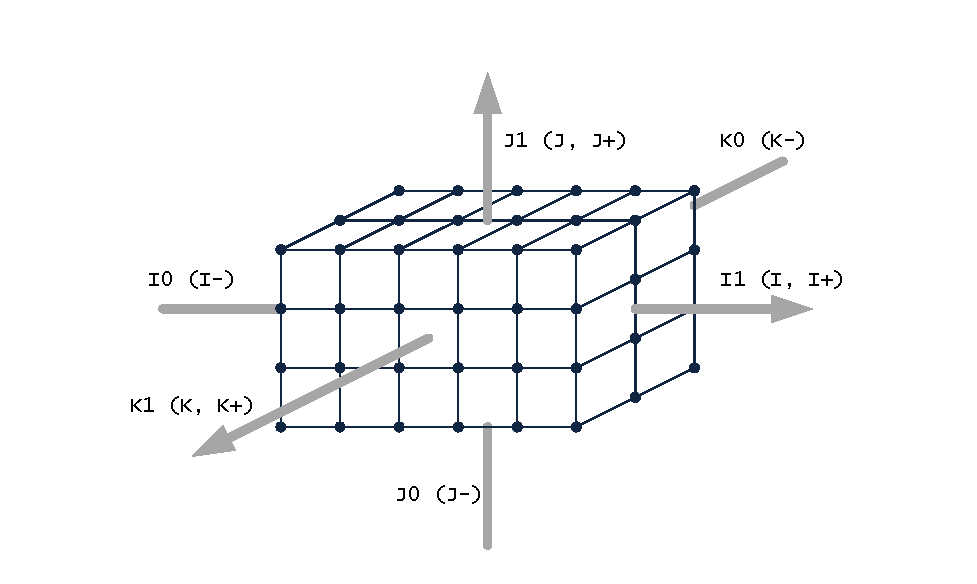
\includegraphics[width=0.45\textwidth]{./pics/text_2_block/1-block.pdf}
&
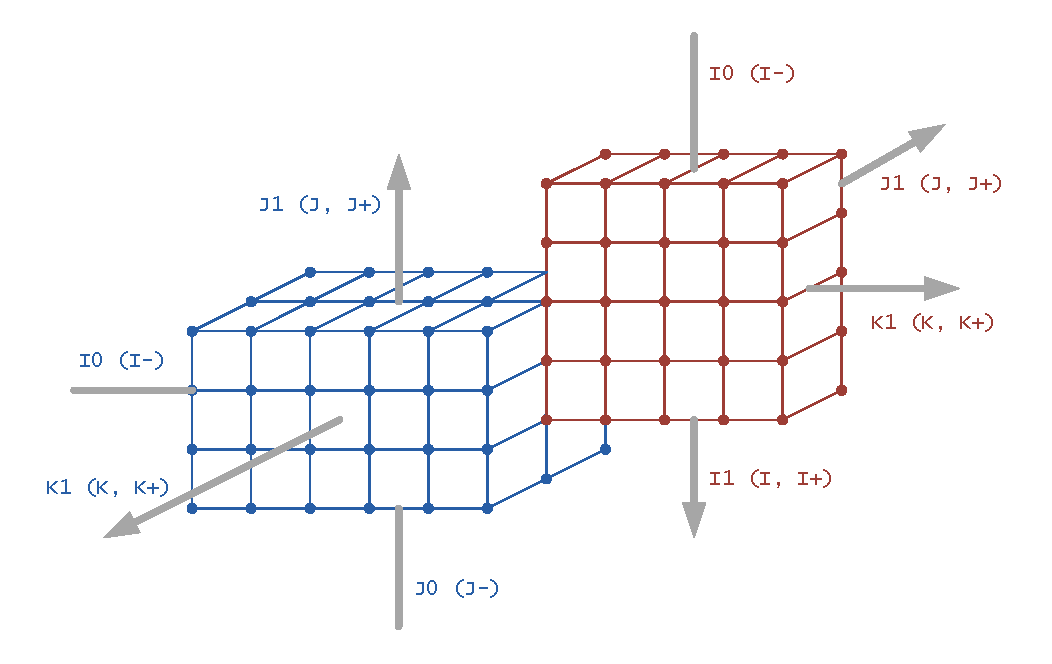
\includegraphics[width=0.45\textwidth]{./pics/text_2_block/2-block-block.pdf}
\end{tabular}
\singlespacing
\captionstyle{center}\caption{Блок сетки (слева) и касание блоков (справа).}
\label{fig:text_2_block_block}
\end{figure}

Блоки могут граничить между собой.

\begin{definition}
Интерфесом\label{term:block_interface} будем называть описание области границы одного блока, по которой он касается другого блока расчетной сетки.
\end{definition}

Один интерфейс описывает соприкосновение двух блоков прямоугольными подобластями своих граней.
При этом системы координат двух соседних блоков не обязаны согласовываться между собой.
Пример касания двух блоков приведен на рис.~\ref{fig:text_2_block_block} справа.

Выполнение расчетов на сетке носит итерационный по времени характер.
Для каждой итерации по времени выполняется пересчет данных ячеек согласно той или иной вычислительной схеме.
Во время обработки одной ячейки возникает потребность обращаться за данными к другим ячейкам (например, для выполнения аппроксимации частных производных каких-либо величин), находящимся рядом с рассматриваемой (в простейшем случае это просто соседние по граням ячейки, но могут использоваться и используются более сложные структуры).

\begin{definition}
Совокупность ячеек расчетной сетки, данные которых используются при обработке конкретной ячейки, называют вычислительным шаблоном, или вычислительной молекулой, или вычислительной окрестностью этой ячейки\label{term:cell_calc_template}.
\end{definition}

На рис.~\ref{fig:text_2_block_cell_delta} показаны примеры вычислительных окрестностей ячейки.

\begin{figure}[ht]
\centering
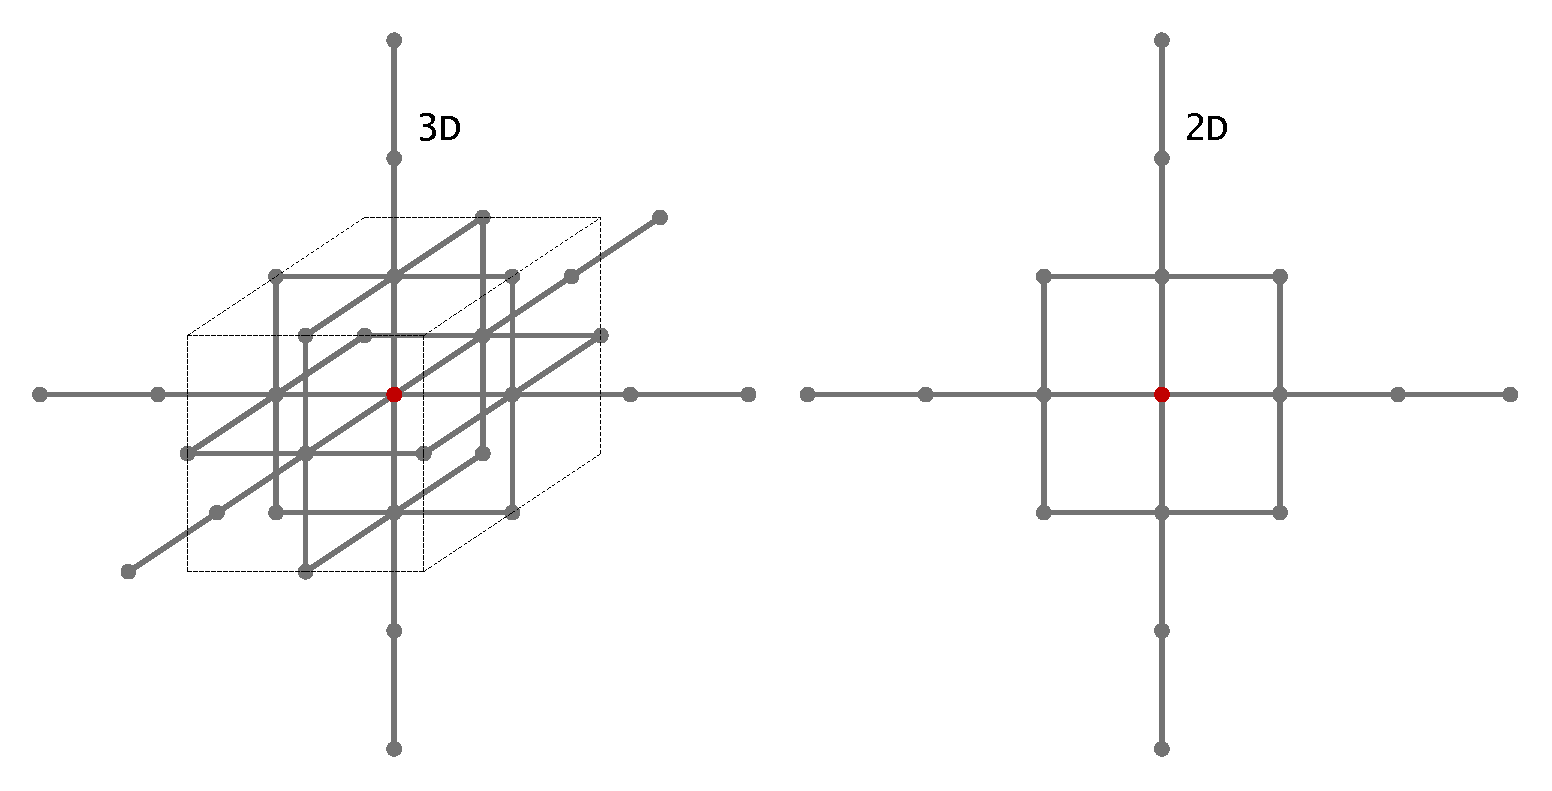
\includegraphics[width=0.8\textwidth]{./pics/text_2_block/3-cell-delta.pdf}
\singlespacing
\captionstyle{center}\caption{Примеры вычислительных окрестностей ячеек сетки.}
\label{fig:text_2_block_cell_delta}
\end{figure}

В дальнейшем для большей наглядности будем изображать блоки в двумерном виде (с системой координат $IJ$).

Во время произведения расчетов различные блоки сетки обрабатываются независимо друг от друга.
При этом для некоторых ячеек обрабатываемого блока их вычислительные окрестности выходят за границу блока и затрагивают соседние блоки.
Для эффективного счета необходимо обеспечить функционал быстрого обмена данными между блоками.
Если два соседних блока обрабатываются на разных узлах суперкомпьютерного кластера, то для обмена данными между ними нужно использовать MPI обмены.
Приведем классификацию ячеек внутри блока сетки (см. рис.~\ref{fig:text_2_block_block_cells}) слева.

\begin{figure}[ht]
\centering
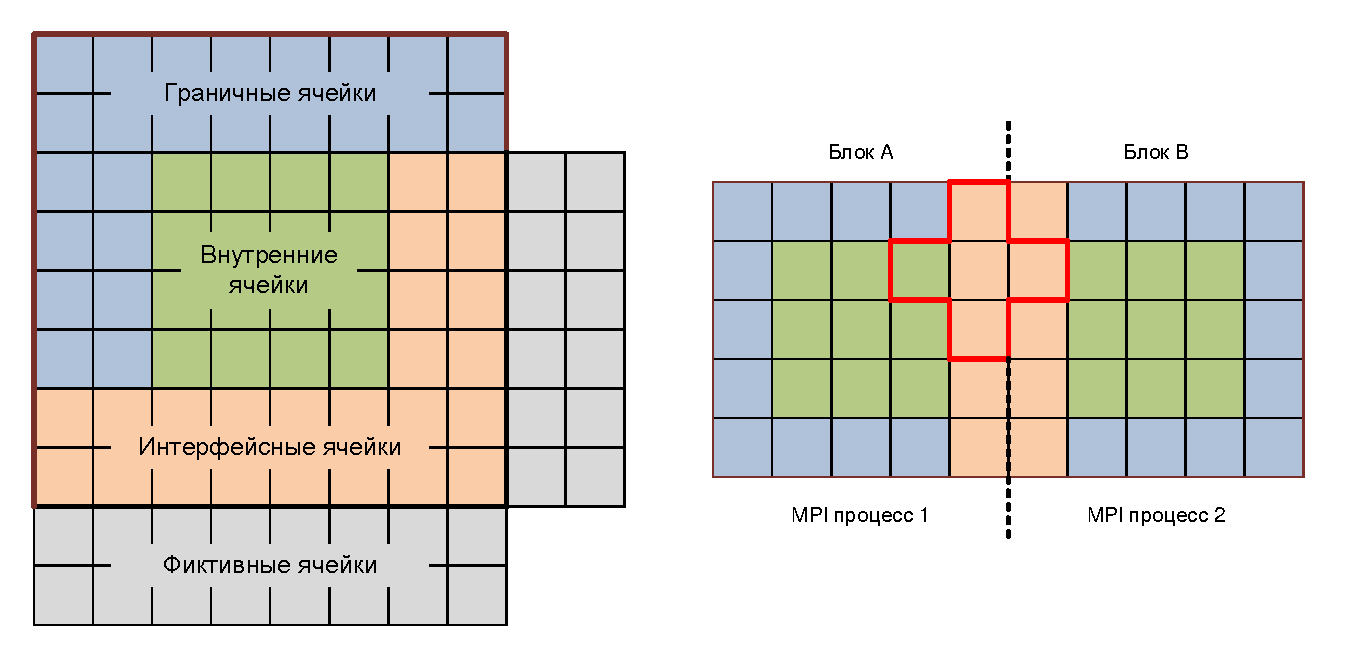
\includegraphics[width=0.8\textwidth]{./pics/text_2_block/4-block-cells.pdf}
\singlespacing
\captionstyle{center}\caption{Ячейки разных типов.}
\label{fig:text_2_block_block_cells}
\end{figure}

\begin{definition}
Внутренними ячейками\label{term:cell_block_inner} (Inner Cells) будем называть те ячейки блока, вся окрестность которых лежит внутри того же блока.
\end{definition}

\begin{definition}
Ячейки, не являющиеся внутренними ячейками блока, будем называть граничными ячейками\label{term:cell_block_border} (Border Cells).
\end{definition}

\begin{definition}
Если окрестность ячейки частично накрывает один из соседних блоков, то такую ячейку будем относить к интерфейсным ячейкам\label{term:cell_block_interface} (Interface Cells), так как ее окрестность пересекает интерфейс блока.
\end{definition}

\begin{definition}
Если окрестность ячейки частично накрывает некоторый блок, который обрабатывается в другом узле суперкомпьютера, то будем относить ее к ячейкам MPI обмена (MPI Cells)\label{term:cell_block_mpi}, так как для получения данных этой окрестности нужно использовать средства межпроцессного обмена (см. рис.~\ref{fig:text_2_block_block_cells} справа).
\end{definition}

При обработке ячеек MPI обмена мы должны обращаться за данными к другому процессу.
Если делать это только по мере необходимости, то придется совершать большое количество обменов, что негативно скажется на производительности.
Поэтому для повышения быстродействия вместо этого для блока заводится специальный слой внешних ячеек, куда копируются все необходимые данные из соседних процессов, которые могут понадобиться при обработке блока.
Такие ячейки будем называть фиктивными\label{term:cell_block_ghost}.

\begin{definition}
Фиктивными ячейками блока будем называть дополнительно созданные для этого блока ячейки, которые содержат скопированные из соседних блоков данные, необходимые для выполнения вычислений в рассматриваемом блоке.
Множество фиктивных ячеек блока также будем называть его теневым слоем\label{term:block_shadow_layer}.
\end{definition}

Ширина теневого слоя блока определяется размером вычислительного шаблона обработки ячейки.
Фиктивные ячейки могут не являться ячейками в физическом смысле, так как для проведения вычислений необходимы не все данные фиктивных ячеек, но на логическом уровне будем изображать их отдельными ячейками.
Таким образом, объединение всех ячеек блока с множеством фиктивных ячеек является замкнутой структурой, которая более не требует для своей обработки обращений к другим MPI процессам (на одной итерации выполнения расчетов).

Далее опишем основные объекты, используемые для организации работы с блочно-структурированной сеткой, способы описания этих объектов и внутренние структуры, позволяющие эффективно оперировать этими объектами и производить вычисления.

\subsubsection{Основные объекты блочно-структурированной сетки}

В рамках проведения исследований по распараллеливанию вычислений на блочно-структурированных сетках была разработана архитектура расчетной сетки, реализованы ее объекты и инструменты для работы с ней \cite{CertRybakov2020PrepStruct}.

Основным объектом блочно-структурированной расчетной сетки является блок (Block) (см. рис.~\ref{fig:text_2_block_block_and_coords}). 
Блок состоит из трехмерного массива ячеек размера $IS \times JS \times KS$.
Каждая ячейка содержит набор газодинамических параметров, ассоциированных с центром масс ячейки и другие вспомогательные данные.
Также блок содержит данные о всех вершинах своих ячеек, эти данные хранятся в трехмерном массиве размера $(IS + 1) \times (JS + 1) \times (KS + 1)$.

Для определения геометрии блока необходимо задать его линейные размеры и координаты ($X$, $Y$, $Z$) всех его узлов.

\begin{figure}[ht]
\centering
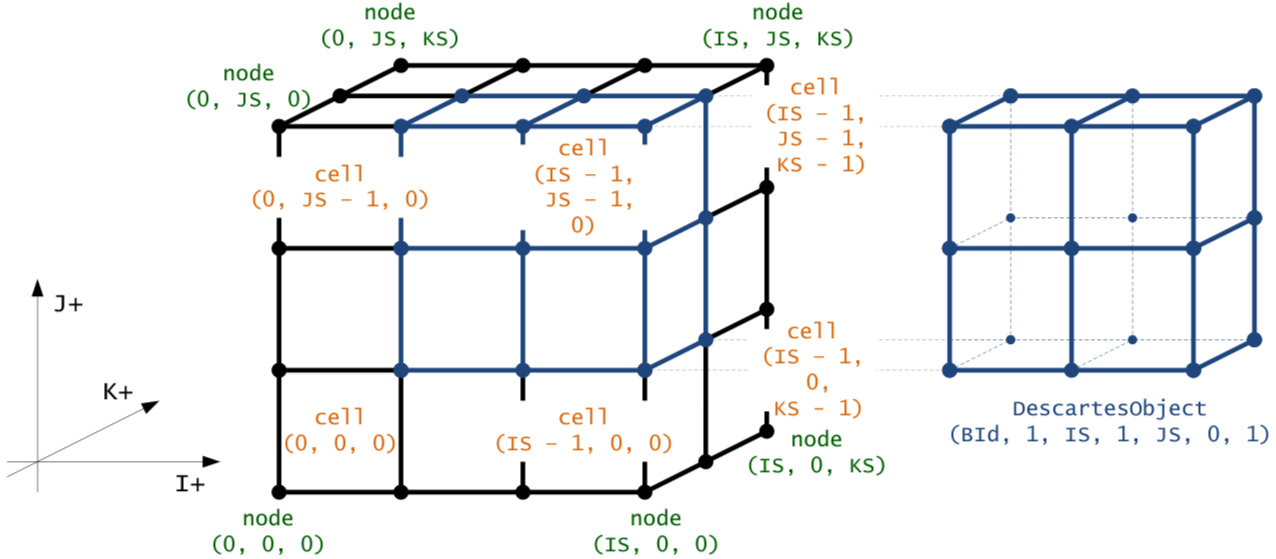
\includegraphics[width=0.7\textwidth]{./pics/text_2_block/6-block-and-coords.png}
\singlespacing
\captionstyle{center}\caption{Блок сетки и координаты его узлов.}
\label{fig:text_2_block_block_and_coords}
\end{figure}

\begin{figure}[ht]
\centering
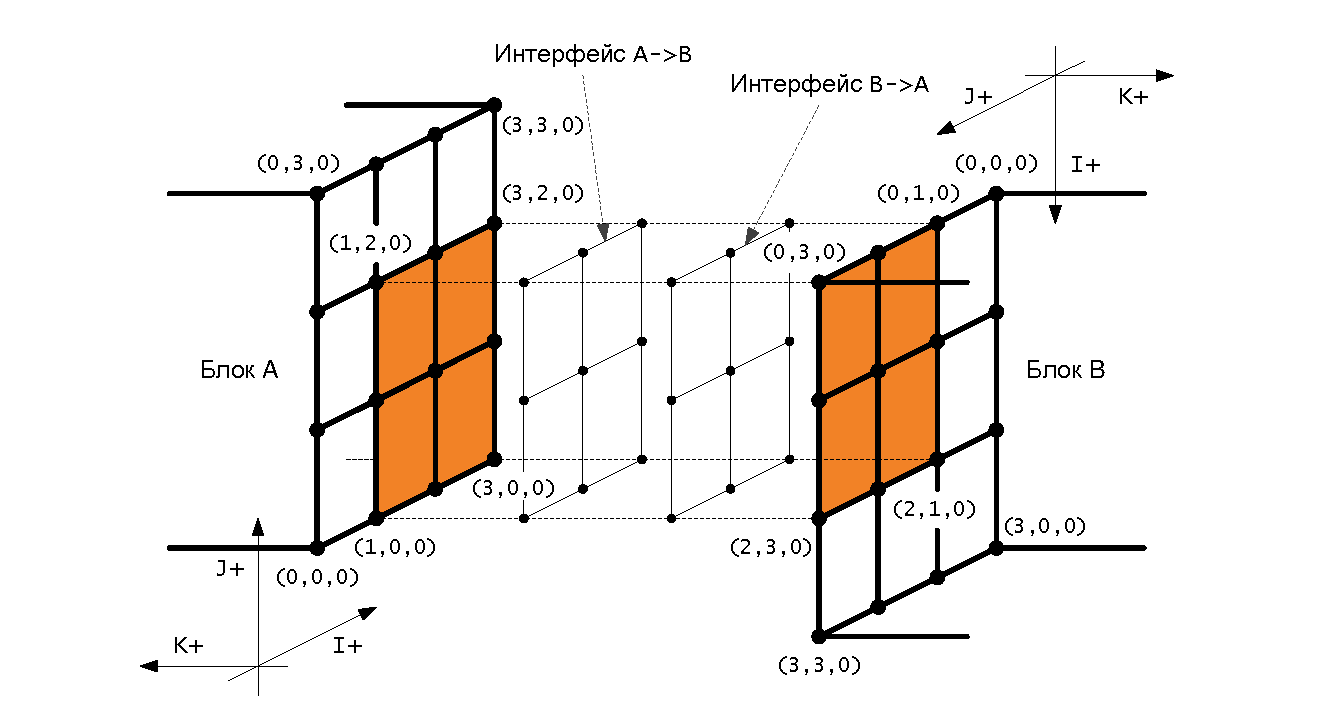
\includegraphics[width=0.8\textwidth]{./pics/text_2_block/7-iface.pdf}
\singlespacing
\captionstyle{center}\caption{Структура интерфейса касания блоков.}
\label{fig:text_2_block_iface}
\end{figure}

Объектом, описывающим соприкосновение двух соседних блоков, является интерфейс (Iface) (см. рис.~\ref{fig:text_2_block_iface}).
Интерфейс является однонаправленным, он сообщает, что у данного блока конкретная прямоугольная
часть границы соприкасается с другим блоком.
Чтобы определить с какой частью другого блока граничит рассматриваемый блок, нужно рассмотреть смежный ему интерфейс.
Таким образом полная информация о касании двух соседних блоков описывается парой смежных интерфейсов.

Интерфейс описывает только касание по ненулевой площади (касание по узлу или ребрам ячеек не рассматривается).
Также возможно обоюдное касание друг друга разных граней одного и того же блока, хотя такие случаи нужно рассматривать отдельно, так как самокасание может потребовать специальной обработки блоков при управлении сеткой.
В общем случае самокасания блоков рекомендуется избегать.

Интерфейс описывается в системе координат того блока, к которому он относится.
Координаты задают размер области соприкосновения по всем трем направлениям.

В приведенном на рис.~\ref{fig:text_2_block_iface} примере два смежным интерфейса, описывающих касание блоков A и B задаются следующим образом: $A(1, 3, 0, 2, 0, 0) \rightarrow B$, $B(0, 2, 1, 3, 0, 0) \rightarrow A$.

\begin{figure}[ht]
\centering
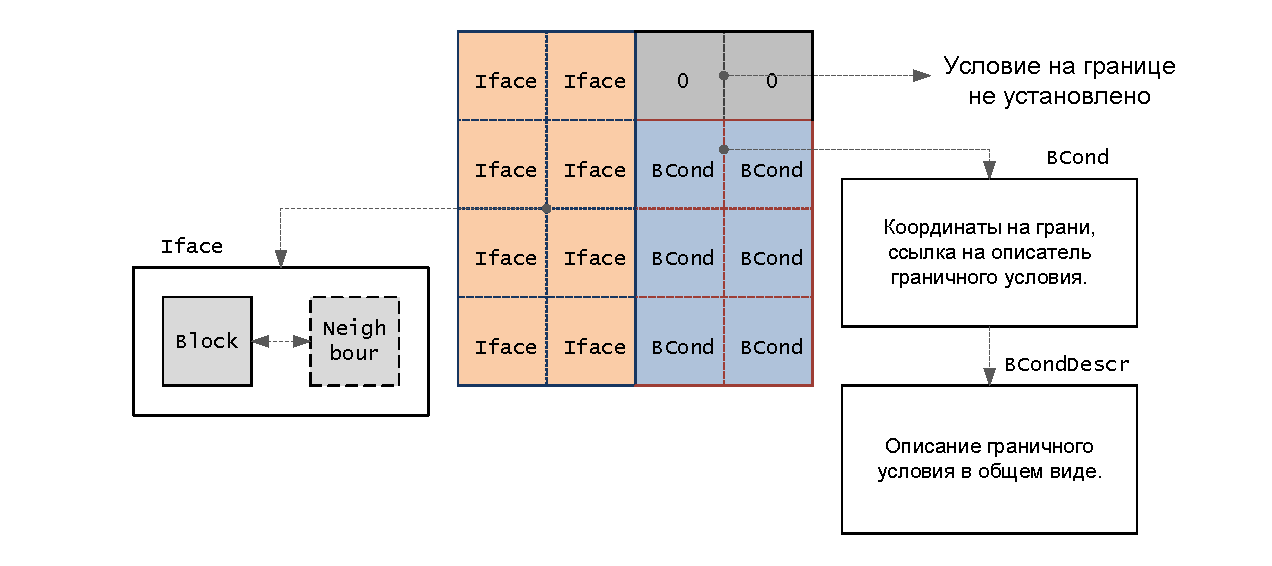
\includegraphics[width=0.8\textwidth]{./pics/text_2_block/8-facet.pdf}
\singlespacing
\captionstyle{center}\caption{Структура грани блока.}
\label{fig:text_2_block_facet}
\end{figure}

То есть для одного интерфейса задается блок, которому этот интерфейс принадлежит, координаты интерфейса в данном блоке и соседний блок.
Этой информации достаточно чтобы полностью определить геометрию касания блоков.
Направление интерфейса можно определить по той координате, протяженность интерфейса по которой равна нулю (в данном случае это координата $K$).
Остается определить только каким образом системы координат двух соседних блоков соотносятся друг с другом.
Это можно сделать, зная координаты узлов соответствующих блоков.

На границе блока кроме другого блока может находиться граница расчетной области.
В этом случае на границе блока необходимо задать граничные условия (BCond).
Граничные условия задаются аналогично интерфейсу (с помощью системы координат блока), однако вместо соседнего блока подается ссылка на описатель граничных условий.
Таким образом и интерфейс и граничное условие являются частным случаем границы блока (Border).

В процессе вычислений необходимо иметь возможность быстро узнать для конкретной граничной ячейки, какого типа граница ей соответствует и быстро найти соответствующий интерфейс или граничное условие.
Для этой цели служат грани блока (Facet)\label{term:block_facet}.
Каждый блок имеет 6 граней (для каждого из направлений $I-$, $I+$, $J-$, $J+$, $K-$, $K+$).
Каждая грань является двумерным массивом, содержащим для каждой ячейки, граничащей с гранью, ссылку на интерфейс или на граничное условие (см. рис.~\ref{fig:text_2_block_facet}).

Важным объектом сетки является область блока (Scope)\label{term:block_scope}.
Области нужны для описания начальных условий.
Область блока в целом аналогична граничному условию за исключением того, что является трехмерным объектом.
Область блока задается в системе координат блока, имеет ненулевую протяженность по каждому направлению и ссылается на описатель начальных условий.
Структура описателя начальных условий полностью аналогична описателю граничных условий.

Таким образом, все основные рассмотренные объекты сетки являются двумерными или трехмерными декартовыми объектами, то есть такими объектами, чья геометрия задается двумерными или трехмерными массивами узлов блоков сетки.
Также заметим, что граничные условия и области являются именованными объектами, так как им присваиваются имена для определения механизмов задания граничных и начальных условий расчета.
Исходя из этого, получаем следующую иерархию классов, реализующих расчетную сетку (см. рис.~\ref{fig:text_2_block_hierarchy}).

\begin{figure}[ht]
\centering
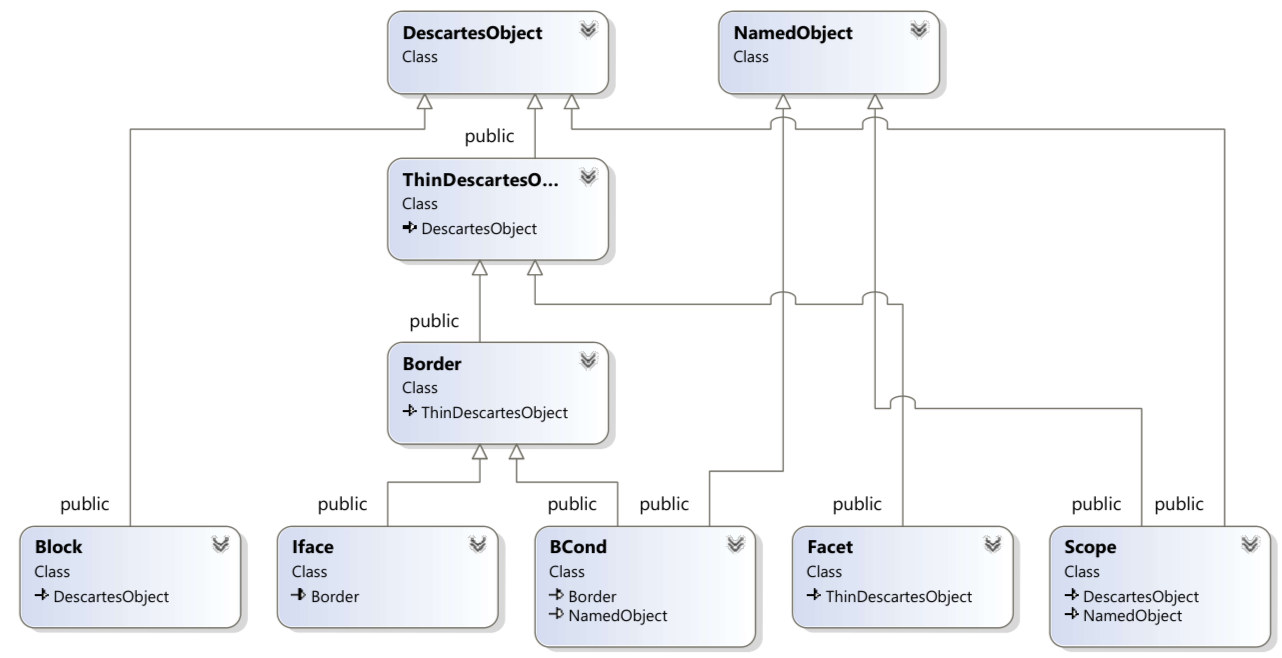
\includegraphics[width=0.8\textwidth]{./pics/text_2_block/9-hierarchy.png}
\singlespacing
\captionstyle{center}\caption{Иерархия объектов внутреннего представления сетки.}
\label{fig:text_2_block_hierarchy}
\end{figure}

\subsubsection{Организация межпроцессных обменов данными между \\ блоками сетки}

Рассмотрим механизм обмена данными между блоками сетки.
Как уже упоминалось, если два соседние блока, между которыми должен быть осуществлен обмен данными, обрабатываются в разных процессах при выполнении расчетов на суперкомпьютере, то обмен данными может быть осуществлен с помощью MPI\label{abbr:mpi2} пересылок.
При этом каждый блок должен отправить своим соседям только данные, находящиеся в его интерфейсных ячейках (могут существовать интерфейсные ячейки, данные из которых требуется отправить сразу двум или трем блокам).
Получить же должен блок те данные, которые соответствуют ячейкам его теневого слоя.

Логика обменов устроена следующим образом.
Так как пара смежных интерфейсов определяет факт касания двух блоков, между которыми должен произойти обмен, то на каждом из этих интерфейсов заводится буфер для данных обмена, после чего происходит обмен данными буферами (см. рис.~\ref{fig:text_2_block_data_exchange}).
Обмены данными происходят одновременно по всем интерфейсам сетки с помощью асинхронных функций
\texttt{MPI\_Isend}, \texttt{MPI\_Irecv}.
Рассмотрим механизм обмена данными между соседними блоками, находящимися в разных процессах, более подробно.

\begin{figure}[ht]
\centering
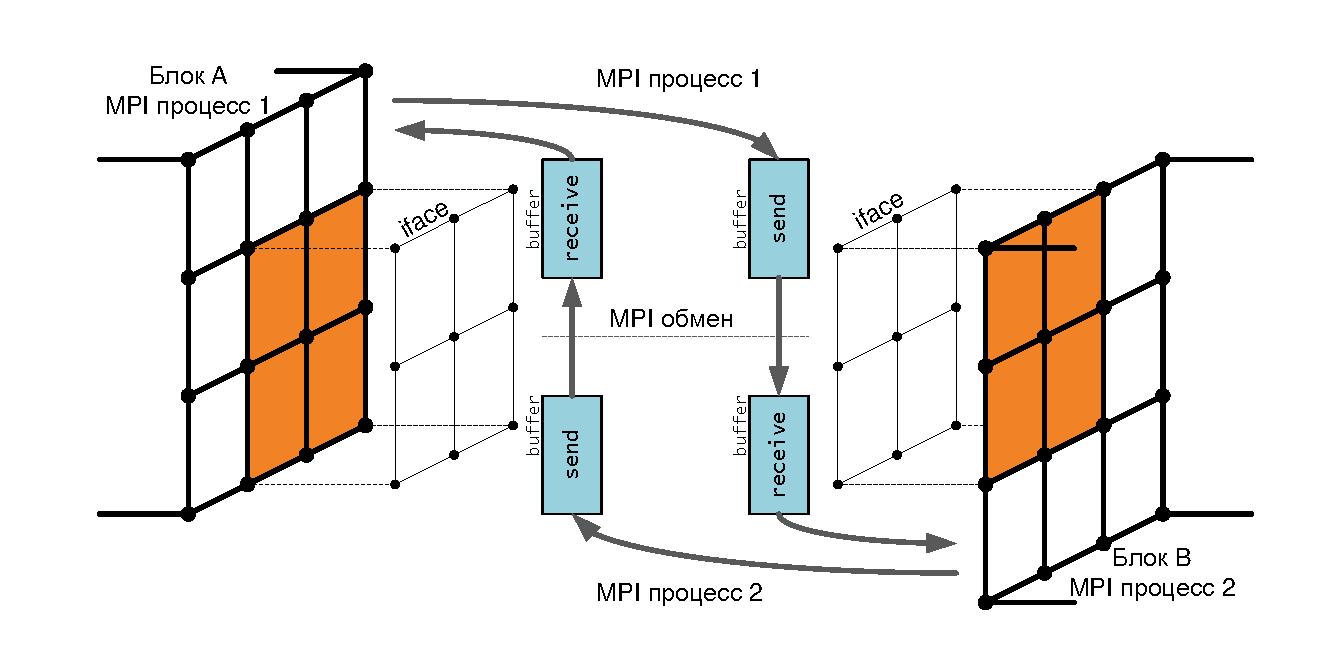
\includegraphics[width=0.8\textwidth]{./pics/text_2_block/10-data-exchange.pdf}
\singlespacing
\captionstyle{center}\caption{Обмен данными между блоками сетки.}
\label{fig:text_2_block_data_exchange}
\end{figure}

Пусть Блок A обрабатывается в процессе 1, а блок B -- в процессе 2, как показано на рис.~\ref{fig:text_2_block_data_exchange}.
Каждый из двух смежных интерфейсов, описывающих касание этих двух блоков имеет свой буфер обмена данными.
Так как в процессе 1 активным является блок A, то буфер его интерфейса работает на прием данных, а буфер интерфейса со стороны блока B -- на отправку (данных блока A).
В процессе 2 все происходит ровно наоборот: активным является блок B, буфер интерфейса блока A работает на отправку данных блока B, буфер интерфейса со стороны блока B работает на прием данных.
Для всех интерфейсов происходит асинхронный запуск всех вызовов функций обмена, после чего происходит ожидание завершения всех операций.
После этого каждый блок может извлечь данный из буфера интерфейса, в котором он является активным, и поместить эти данные в свою теневую зону, после чего начинается следующая итерация расчетов.

\begin{figure}[ht]
\centering
\begin{tabular}{l}
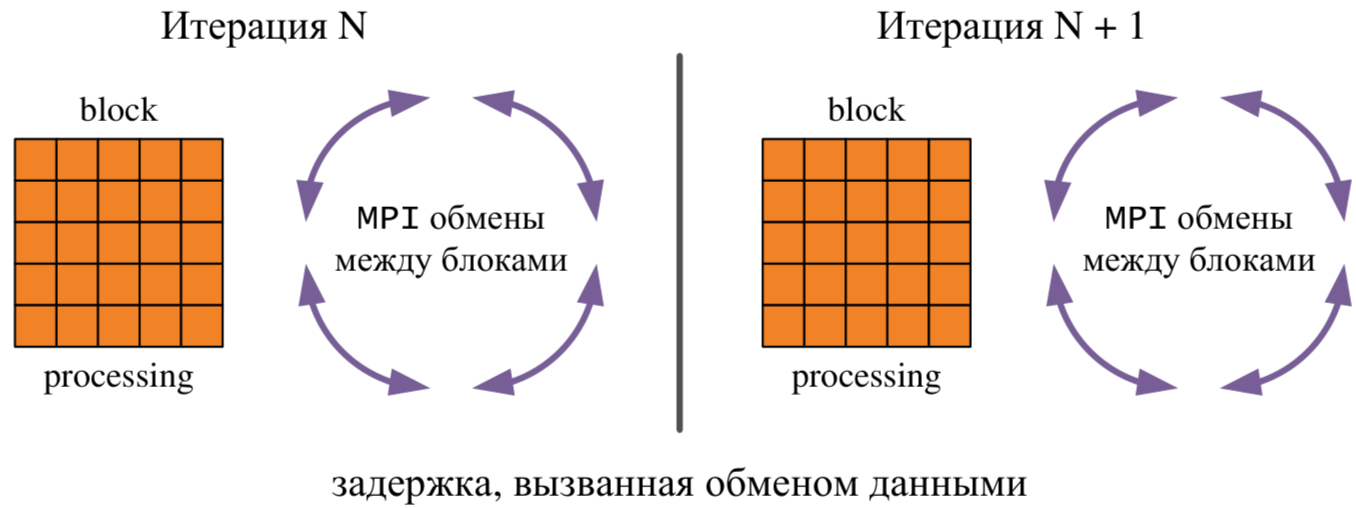
\includegraphics[width=0.6\textwidth]{./pics/text_2_block/11-mpi1.png}
\\
\\
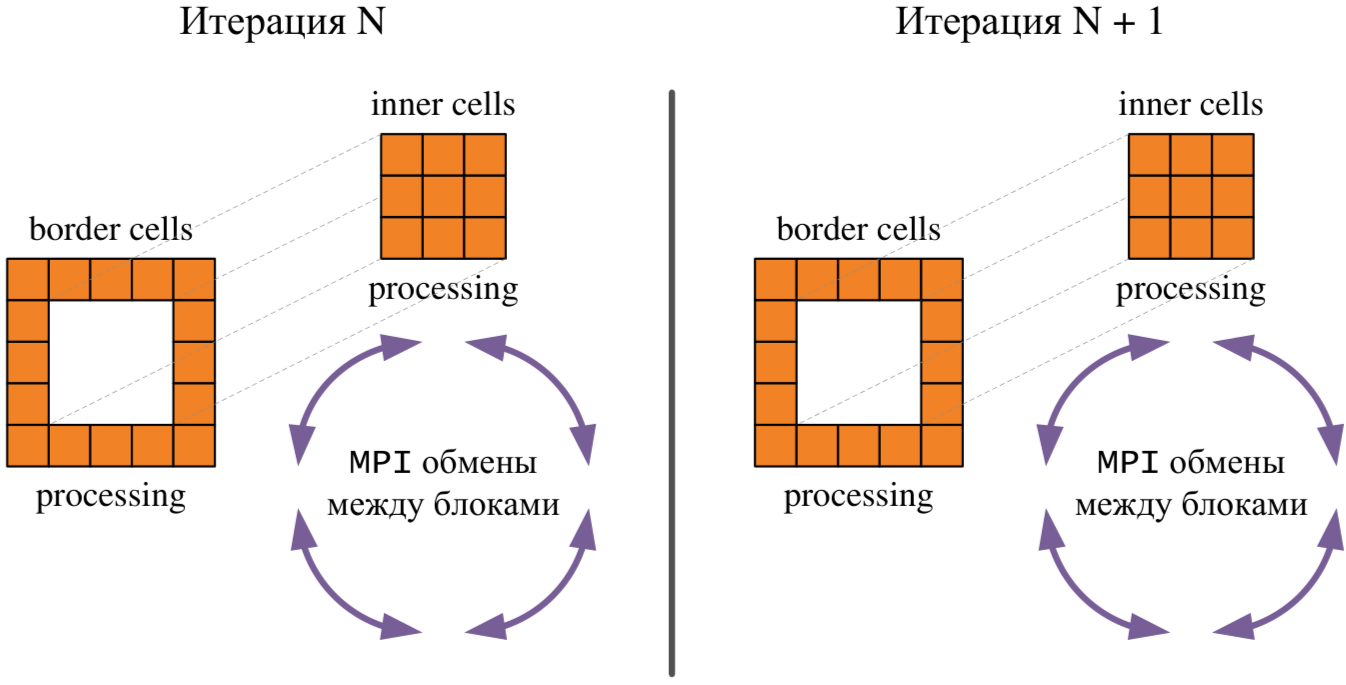
\includegraphics[width=0.6\textwidth]{./pics/text_2_block/12-mpi2.png}
\end{tabular}
\singlespacing
\captionstyle{center}\caption{Задержки, вызванные MPI обменами и избавление от них.}
\label{fig:text_2_block_mpi1}
\end{figure}

После проведения каждой итерации счета задачи необходимо выполнять обмен данными, чтобы состояния граничных ячеек блоков были актуальными.
При этом начинать обсчет следующей итерации нельзя до завершения всех обменов.
Это может привести к возникновению задержек (см. рис.~\ref{fig:text_2_block_mpi1}, сверху).
Чтобы избежать такого рода потери вычислительного времени можно разделить обработку ячеек блока на отдельную обработку всех внутренних ячеек и обработку граничных ячеек.
Сначала нужно произвести обработку всех граничных ячеек блока, затем инициировать асинхронные обмены данными (в которых участвуют только граничные ячейки), а затем сразу начать обработку внутренних ячеек, для которых получение данных фиктивных ячеек не требуется.
Такой подход позволяет скрыть издержки на коммуникацию за полезными вычислениями (см. рис.~\ref{fig:text_2_block_mpi1}, снизу).

Особенности структуры и реализации внутреннего представления блочно-структурированной сетки имеют большое значение для выполнения расчетов на этой сетке.
Правильный выбор объектной модели сетки, способы расположения данных в памяти и другие факторы напрямую влияют на эффективность выполнения программы.
Важную роль в скорости выполнения расчетов играет реализация механизма обмена данными в случае запуска вычисления на суперкомпьютере.
Так как обмен данными должен происходить на каждой итерации вычислений, то это является узким местом для повышения эффективности расчетов.

% Распределение вычислительной нагрузки между узлами гетерогенного вычислительного кластера.
\subsubsection{Распределение вычислительной нагрузки между \\ узлами гетерогенного вычислительного кластера}\label{sec:text_2_getero}

\label{term:cluster_getero}Рассмотрим фиксированную декомпозированную расчетную задачу.
Это могут быть вычисления, выполняемые на блочно-структурированной расчетной сетке, либо на неструктурированной сетке, разбитой на домены.
При распределении частей расчетной задачи между вычислителями суперкомпьютерного кластера для уменьшения времени выполнения задачи важно учитывать характеристики самого кластера, к которым относится производительность вычислителей и скорость обмена данными между ними.
В этом разделе приводится описание эвристического алгоритма распределения вычислительной нагрузки на вычислительном кластере с учетом геометрии расчетной задачи и характеристик кластера \cite{Rybakov2018Distr,Rybakov2017Part}.

\subsubsection{Постановка задачи}

\begin{definition}
Графом вычислительного кластера\label{term:graph_cluster} назовем граф $H = (V_H, E_H)$.
Узлы этого графа соответствуют отдельным вычислителям кластера (одному процессору или сопроцессору), а ребра -- логическим соединениям между вычислителями (то есть возможностью обмена данными).
\end{definition}

Так как между любыми двумя вычислителями возможен обмен данными, то граф $H$ является полным (и даже является псевдографом, так как содержит все возможные петли).
Введем на графе $H$ две весовые функции.
Первая функция $f: V_H \rightarrow \mathbb{R}_{> 0}$ каждому узлу графа ставит в соответствие скорость работы соответствующего вычислителя, то есть количество расчетных данных, которые могут быть обработаны на нем за одну условную единицу времени (для разных вычислительных задач функции могут различаться).
Вторая функция $l: E_H \rightarrow \mathbb{R}_{> 0}$ несет смысл скорости обмена данными между вычислителями, она показывает количество данных, которые могут быть переданы между соответствующими вычислителями за одну условную единицу времени.

\begin{definition}
Графом расчетной задачи\label{term:graph_task} назовем граф $G = (V_G, E_G)$, который отражает особенности декомпозиции расчетной области (это может быть граф блочно-структурированной расчетной сетки или граф доменов неструктурированной сетки).
Узлы этого графа соответствуют расположенным в пространстве множествам данных, каждое из которых обрабатывается одним вычислителем.
Ребра графа соответствуют потокам данных между разными частями задачи.
\end{definition}

На графе $G$ также вводятся две весовые функции.
Первая функция $w: V_G \rightarrow \mathbb{R}_{> 0}$ имеет значение объема вычислительных данных, обрабатываемых в соответствующей части задачи.
Вторая функция $i: E_G \rightarrow \mathbb{R}_{> 0}$ отражает объем данных, пересылаемых между частями задачи при межпроцессном обмене.
Значения всех четырех функций $f$, $l$, $w$, $i$ измеряются в одних и тех же единицах (это могут быть ячейки расчетной сетки, количество байтов или вещественных значений).
Однако $w$ и $i$ имеют смысл объема вычислений и пересылок, тогда как функции $f$ и $l$ относятся к фиксированной единице времени, то есть имеют смысл скорости обработки и пересылки данных.

Расчет задачи состоит из двух чередующихся фаз: проведение итерации расчета и выполнение межпроцессных обменов данными.
Будем считать, что эти фазы не перемешиваются для отдельных частей задачи (хотя возможно выполнять расчеты для одной части задачи и одновременно проводить межпроцессные обмены для другой ее части).
Требуется таким образом распределить задачу между вычислителями кластера, чтобы суммарное время одной итерации расчета и одной итерации межпроцессных обменов было минимально.
Распределение задачи между вычислителями кластера определяется функцией $\gamma: V_G \rightarrow V_H$.

Время выполнения одной итерации вычислений определяется по самому загруженному вычислителю:
\begin{equation}
	t_1^{max} = \max_{v_H \in V_H}{\left( \frac{1}{f(v_H)} \sum_{\substack{v_G \in V_G \\ \gamma(v_G) = v_H}}{w(v_G)} \right)}
\end{equation}

Аналогично время выполнения одной итерации межпроцессных обменов определяется по самому загруженному каналу обмена:
\begin{equation}
	t_2^{max} = \max_{e_H \in E_H}{\left( \frac{1}{l(e_H)} \sum_{\substack{e_G = (u_G, v_G) \in E_G \\ (\gamma(u_G), \gamma(v_G)) = e_H}}{i(e_G)} \right)}
\end{equation}

Таким образом, задача поиска оптимального распределения задачи по вычислителям кластера сводится к поиску функции $\gamma$, минимизирующей значение функционала $t^{max}(\gamma) = t_1^{max}(\gamma) + t_2^{max}(\gamma)$.
Так как каждый элемент из множества $V_G$ может быть отнесен к любому вычислителю, то общее количество всех функций распределения равно $|V_H|^{|V_G|}$.

Можно рассматривать частные случае задачи распределения вычислительной нагрузки.
Для вычислительных задач с малой долей мепроцессных обменов можно ограничиться минимизацией функционала $t^{max}(\gamma) = t_1^{max}(\gamma)$.
Также можно рассматривать задачу распределения для гомогенного кластера\label{term:cluster_gomo}, для которого функции $f$ и $l$ являются константами.
Минимизируемый функционал в этом случает принимает следующий вид:
\begin{equation}
	t^{max}(\gamma) =
		\frac{1}{f} \max_{v_H \in V_H}{\left( \sum_{\substack{v_G \in V_G \\ \gamma(v_G) = v_H}}{w(v_G)} \right)} + 
		\frac{1}{l} \max_{e_H \in E_H}{\left( \sum_{\substack{e_G = (u_G, v_G) \in E_G \\ (\gamma(u_G), \gamma(v_G)) = e_H}}{i(e_G)} \right)}
\end{equation}

Рассмотрим эвристический алгоритм поиска приближенного решения поставленной задачи, который учитывает весовые функции графов задачи и вычислительного кластера, а также геометрию расчетной области задачи.

\subsubsection{Описание алгоритма}

Одной из особенностей вычислительного кластера является то, что скорость обмена данными между двумя частями задачи, обрабатываемыми одним вычислителем, существенно выше, чем скорость обмена данными между двумя частями задачи, обрабатываемыми двумя разными вычислителями.
Интуитивно понятно, что задача должна распределяться между узлами вычислительного кластера таким образом, чтобы расположенные рядом части задачи попадали на один вычислитель.
В идеале граф $G$ задачи должен быть разбит на $|V_H|$ связных партиций, каждая из которых обрабатывается своим вычислителем, причем вес партиции (суммарный вес частей задачи, входящих в партицию), должен быть пропорционален весу соответствующего вычислителя.

Каждому узлу графа $G$ поставлена в соответствие точка трехмерного пространства (центр соответствующей части расчетной задачи). 
С использованием данных точек формировать партиции можно по геометрическому принципу.
Для этого сначала нужно выполнить первую фазу алгоритма -- определить базовые точки\label{term:distr_base_point}, вокруг которых в дальнейшем будут формироваться партиции.
Базовые точки должны быть распределены по объему расчетной области задачи таким образом, чтобы веса сформированных впоследствии партиций были пропорциональны весам вычислителей.
Будем считать, что все ячейки расчетной сетки, используемой в задаче, имеют примерно равные размеры.
Это означает, что нет заметных сгущений и разряжений сетки.
В условии нашего допущения объем области, занимаемой партицией, будет пропорционален ее весу.
Таким образом, задача определения базовых точек сводится к следующей: требуется в данной области пространства определить такое множество точек, чтобы объемы окрестностей, окружающих эти точки, были пропорциональны весам вершин графа $H$.
При этом окрестность точки строго не определяется.
Главное, чтобы окрестность содержала саму точку и имела интуитивно компактную форму.

Добиться определения базовых точек можно с помощью простого итерационного алгоритма с имитацией взаимного отталкивания точек друг от друга.
Обозначим область расчетной задачи через $\Omega$.
На первом шаге расположим $|V_H|$ точек (будем обозначать их с помощью соответствующих радиус-векторов) случайным образом внутри области $\Omega$.
Каждой базовой точке поставим в соответствие конкретную вершину графа $H$.
Таким образом, каждая точка $\overline{p}(v_H)$ будет иметь вес $f(v_H)$.
Далее на каждом шаге будем моделировать силу взаимного отталкивания между двумя точками $\overline{p}(v_1)$ и $\overline{p}(v_2)$ по закону
\begin{equation}
	F(\overline{p}(v_1), \overline{p}(v_2)) = \frac{f(v_1) f(v_2)}{|\overline{p}(v_1) - \overline{p}(v_2)|^2}
\end{equation}

После этого будем корректировать положение каждой точки под действием суммарной силы отталкивания от всех остальных точек.
Кроме того, суммарную силу нужно дополнить корректирующей силой отталкивания от границ области $\Omega$, иначе все точки будут располагаться на этой границе.
Алгоритм заканчивает свою работу, когда положение точек стабилизируется, что говорит об уравнивании всех моделируемых сил отталкивания.

\begin{figure}[ht]
\centering
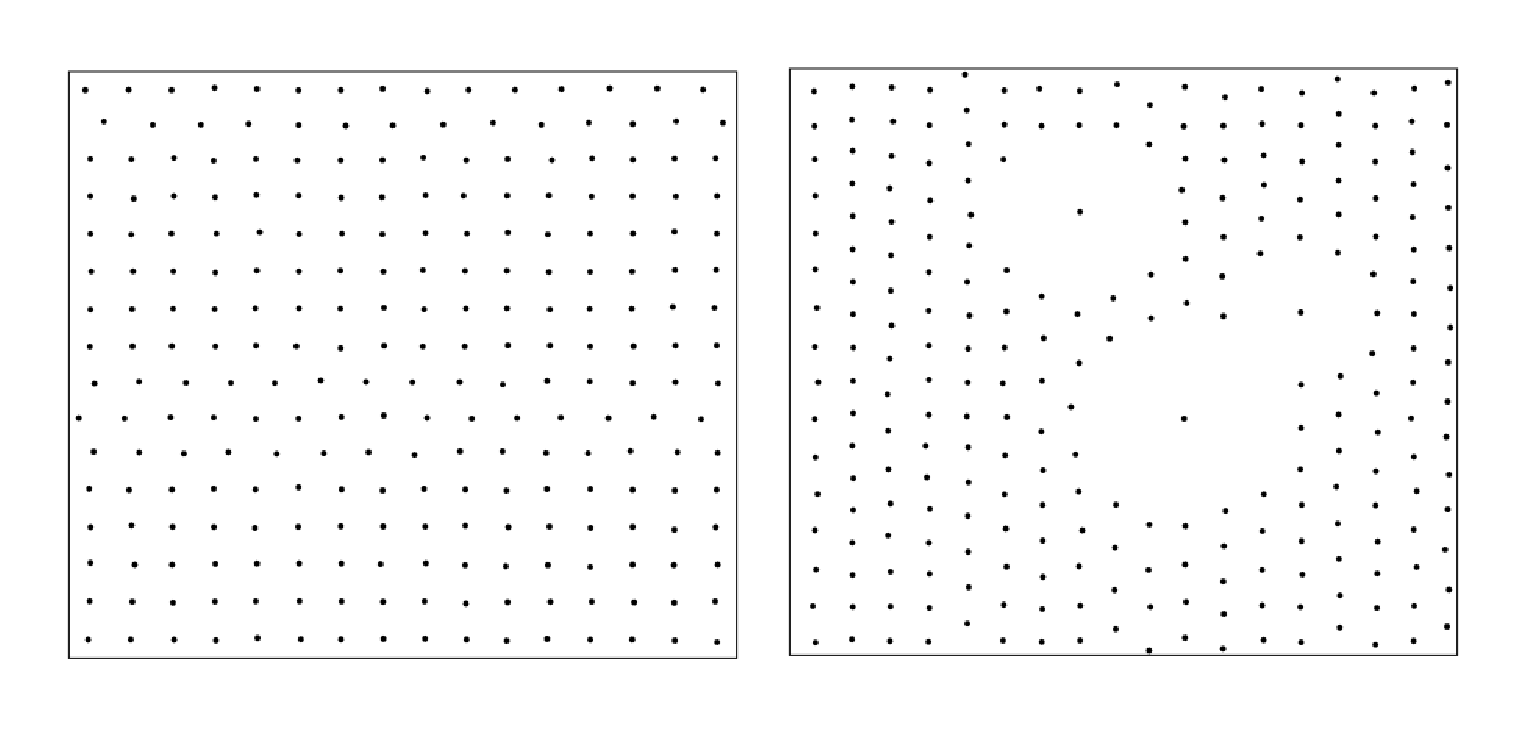
\includegraphics[width=0.7\textwidth]{./pics/text_2_getero/rvp.pdf}
\singlespacing
\captionstyle{center}\caption{Иллюстрация работы алгоритма определения базовых точек.}
\label{fig:text_2_getero_rvp}
\end{figure}

На рис.~\ref{fig:text_2_getero_rvp} показана иллюстрация работы алгоритма определения базовых точек внутри квадратной области в двумерном случае.
На рисунке слева все точки имеют одинаковые веса, на рисунке справа выделены три точки, имеющие случайные веса значительно выше среднего значения.
После определения базовых точек можно переходить ко второй фазе алгоритма -- определение (наращивание) партиций вокруг базовых точек.
На каждом шаге наращивания партиций будем выбирать наименее загруженную партицию, то есть партицию с минимальным значением
\begin{equation}
	\frac{1}{f(v_H)} \sum_{\substack{v_G \in V_G \\ \gamma(v_G) = v_H}}{w(v_G)},
\end{equation}

характеризующим время обработки данных этой партиции на одной итерации расчетов, и добавлять к ней новую вершину из $V_G$.
Если на текущем шаге рассматриваемая партиция пуста, то добавим к ней вершину из $V_G$, расположенную ближе всех к базовой точке $\overline{p}(v_H)$.
Если рассматриваемая партиция уже содержит точки, то рассмотрим ее окрестность.

\begin{definition}
Окрестностью партиции $\delta(v_H)$ назовем множество не входящих в нее (и ни в какую другую партицию) вершин графа $G$, соединенных ребром хотя бы с одной вершиной из этой партиции.
\end{definition}

Выберем из этой окрестности вершину $v \in V_G$ с максимальным показателем предпочтения $q(v)$, который определяется по следующей формуле:
\begin{equation}\label{eqn:text_2_getero_q}
	q(v) = \frac{w(v)}{f(v_H)} +
		\left( \sum_{\substack{e = (u, v) \in E_G \\ \gamma(u) = v_H}}{i(e)} \right) \cdot
		\left( \frac{\sum_{\substack{e_H = (u', v') \in E_H \\ u' \ne v'}}{l(e_H)}}{|E_H| - |V_H|} \right)^{-1}
\end{equation}

Первое слагаемое в \eqref{eqn:text_2_getero_q} отражает время обработки данных из части задачи, соответствующей вершине $v$, на вычислителе $v_H$.
Второе слагаемое отражает время межпроцессных обменов, которое потенциально удастся сократить после добавления в партицию вершины $v$ (при этом в качестве скорости обменов берется среднее значение функции $l$ по всем вершинам графа $H$ за исключением петель).

\begin{figure}[ht]
\centering
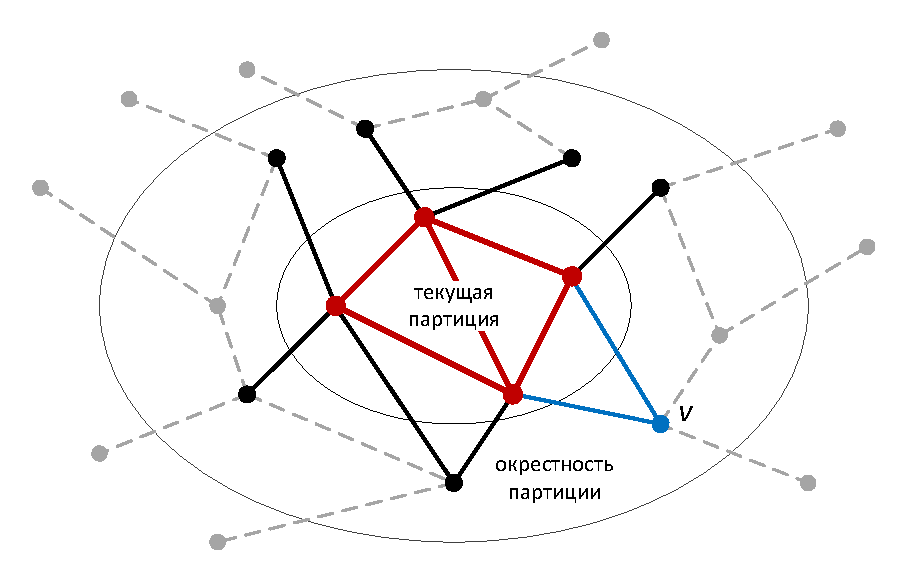
\includegraphics[width=0.6\textwidth]{./pics/text_2_getero/partition.pdf}
\singlespacing
\captionstyle{center}\caption{Добавление новой вершины в партицию.}
\label{fig:text_2_getero_partition}
\end{figure}

На рис.~\ref{fig:text_2_getero_partition} приведена иллюстрация расширения текущей партиции (отмечено красным) за счет добавления новой вершины ($v$).
При этом ребра, отмеченные синим цветом становятся внутренними ребрами партиции, что гарантирует ускорение обмена данными по этим ребрам.

Так как количество вершин в графе $G$ конечно, а на каждом шаге алгоритма в некоторую партицию добавляется одна вершина, то алгоритм заканчивает свою работу, когда все вершины распределены по партициям.

На шаге расширения партиции возможна такая ситуация, когда вся окрестность текущей партиции уже распределена по соседним партициям.
Такое возможно на последних шагах распределения, когда остается малое количество нераспределенных частей задачи.
В этом случае партицию можно расширить просто ближайшей свободной вершиной графа $G$.
Это приводит к тому, что в распределении оказываются отдельные вершины графа $G$, принадлежащие одной партиции, полностью окруженные вершинами из других партиций.
Для корректировки таких неэффективных с точки зрения обмена данными аномалий выполняется третья фаза алгоритма -- захват партициями внутренних точек, на которой партиция может поглотить небольшие анклавы вершин графа $G$.

\subsubsection{Результат работы}

Для анализа эффективности работы описанного алгоритма рассматривалась модельная задача, двумерная квадратная расчетная область которой равномерно разбита близкие по размеру части.
В качестве расчетного кластера рассматривались гомогенный и гетерогенный кластеры, содержащие 8 вычислителей.

\begin{figure}[ht]
\centering
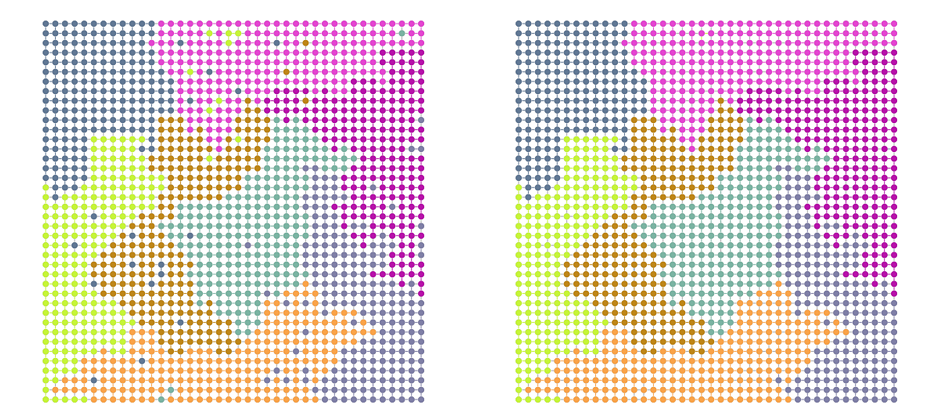
\includegraphics[width=0.8\textwidth]{./pics/text_2_getero/res1small.png}
\singlespacing
\captionstyle{center}\caption{Результат применения алгоритма для распределения вычислительной нагрузки между вычислительного гомогенного кластера.}
\label{fig:text_2_getero_res1}
\end{figure}

На рис.~\ref{fig:text_2_getero_res1} проиллюстрирована работа алгоритма распределения вычислительной нагрузки для модельной задачи между 8 вычислителями гомогенного кластера (то есть все вычислители идентичны).
Слева представлены результаты после второй фазы алгоритма, при этом наблюдается некоторое перемешивание партиций.
Справа показаны результаты после третьей фазы алгоритма, на которой корректируется связность партиций путем поглощения отдельных узлов графа $G$, попавших не в свою партицию.

\begin{figure}[ht]
\centering
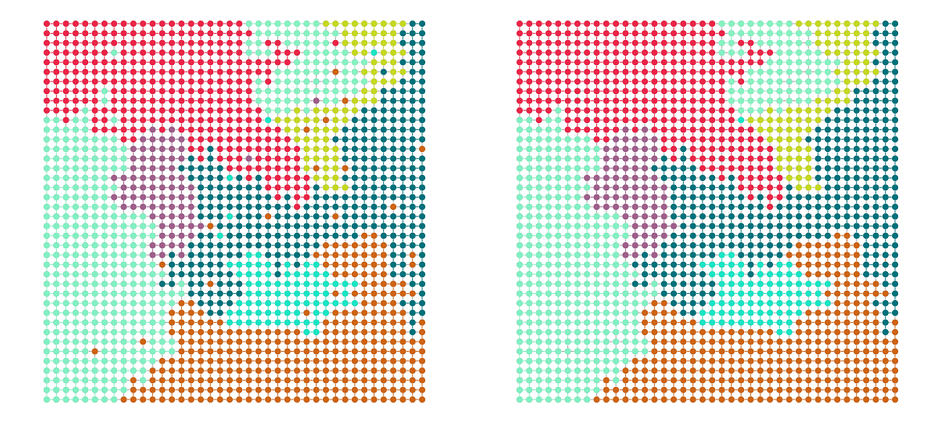
\includegraphics[width=0.8\textwidth]{./pics/text_2_getero/res2small.png}
\singlespacing
\captionstyle{center}\caption{Результат применения алгоритма распределения вычислительной нагрузки между вычислителями гетерогенного кластера.}
\label{fig:text_2_getero_res2}
\end{figure}

На рис.~\ref{fig:text_2_getero_res2} показаны аналогичные результаты работы алгоритма для гетерогенного кластера, состоящего из узлов двух типов, отличающихся по производительности друг от друга в 4 раза.
На иллюстрациях видна разница в размерах партиций, отнесенных к тому или иному типу вычислителя.

Из рис.~\ref{fig:text_2_getero_res1} и рис.~\ref{fig:text_2_getero_res2} видно, что получившиеся партиции имеют довольно протяженные изломанные границы, что негативно влияет на скорость межпроцессных обменов.
Для их сокращения требуется проведение дополнительной фазы алгоритма, состоящей в выравнивании границ (алгоритм сглаживания границ будет рассмотрен в разделе \ref{sec:text_2_smooth}).

Для оценки эффективности алгоритма кроме характеристики времени исполнения одной вычислительной итерации и одной итерации межпроцессных обменов $t^{max}(\gamma)$ расчитывалась аналогичная характеристика
\begin{equation}
	t^{min}(\gamma) =
		\frac{1}{f} \min_{v_H \in V_H}{\left( \sum_{\substack{v_G \in V_G \\ \gamma(v_G) = v_H}}{w(v_G)} \right)} + 
		\frac{1}{l} \min_{e_H \in E_H}{\left( \sum_{\substack{e_G = (u_G, v_G) \in E_G \\ (\gamma(u_G), \gamma(v_G)) = e_H}}{i(e_G)} \right)}
\end{equation}

Разность этих двух значений отражает неэффективность распределения, связанную с простоем вычислительных ресурсов.

Для модельной задачи были проведены эксперименты по распределению графа задачи на узлы гомогенного и гетерогенного кластера при изменении количества вычислителей от 2 до 300.
На рис.~\ref{fig:text_2_getero_chart} представлены полученные зависимости.
Видно, что для обоих видов кластеров при увеличении количества вычислителей наблюдается линейная тенденция к снижению эффективности распределения, но в случае гетерогенного кластера эффективность распределения оказывается ниже.

\begin{figure}[H]
\centering
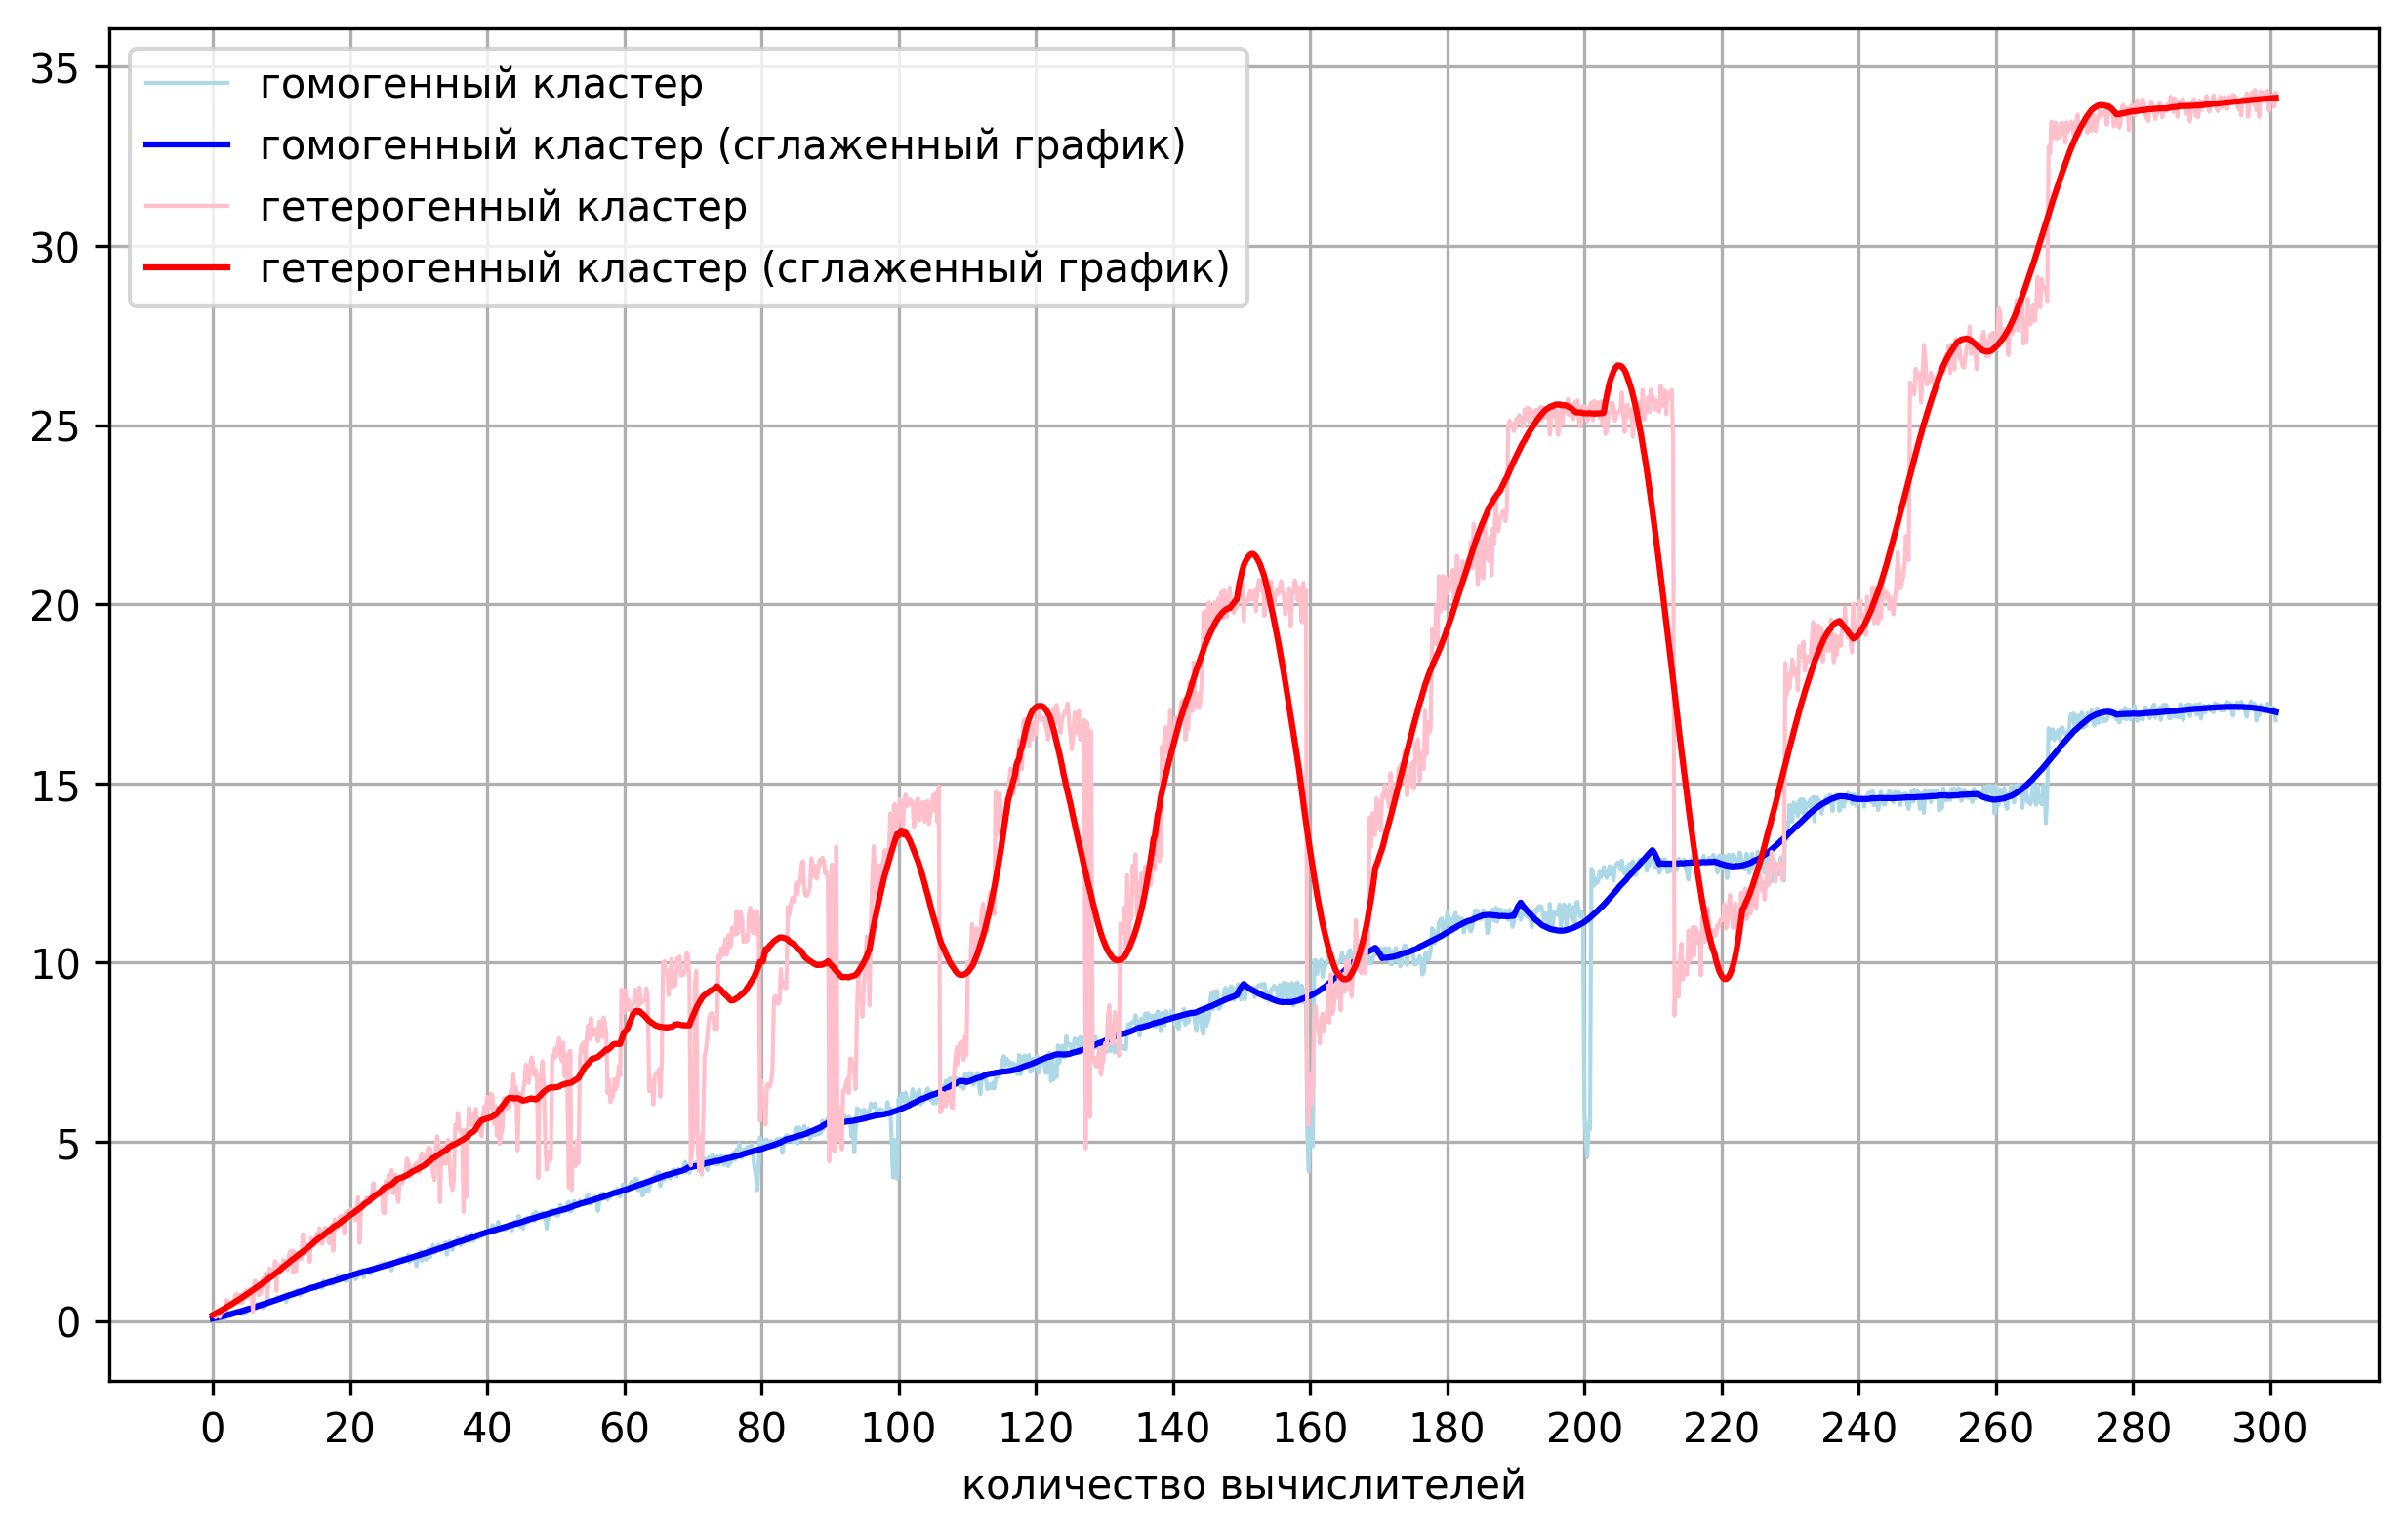
\includegraphics[width=0.8\textwidth]{./pics/text_2_getero/chart2.png}
\singlespacing
\captionstyle{center}\caption{Зависимость показателя эффективности распределения задачи между узлами гомогенного и гетерогенного вычислительных кластеров (по горизонтали отложено количество вычислителей, по вертикали -- значение $\frac{t^{max} - t^{min}}{t^{min}} \cdot 100\%$.}
\label{fig:text_2_getero_chart}
\end{figure}

\subsubsection{Распределение вычислительной нагрузки \\ с дроблением блоков сетки}

При использовании блочно-структурированной расчетной сетки\label{term:mesh_block_struct3} даже оптимальное решение задачи о распределении блоков по вычислиттелям суперкомпьютера не приводит к эффективному выполнению задачи.
При возрастании количества доступных вычислителей скорость работы задача упирается в обработку самого крупного блока.
Для достижения эффективного распределения вычислительной нагрузки требуется выполнять дробление отдельных крупных блоков.
В этом разделе рассмотрены алгоритмы дробления блоков блочно-структурированной расчетной сетки и описаны эксперименты по влиянию дробления блоков на эффективность проведения вычислений.

\subsubsection{Дробление блоков}

Одним из важнейших для распределения вычислительной нагрузки действий по управлению расчетной блочно-структурированной сеткой при выполнении вычислений на суперкомпьютере является дробление ее блоков \cite{Rybakov2016WithCut}.
Так как при запуске задач на суперкомпьютере постоянно возрастает степень параллельности (используется все больше параллельных процессов обработки блоков сетки), то для сохранения равномерности распределения блоков по вычислительным процессам требуется уметь измельчать блоки.
Блок сетки может быть разделен на два блока по любому из трех направлениий: $I$, $J$, $K$.

Кроме блоков сетка содержит другие объекты, которые требуют корректировки после разделения блока.
Сюда относятся интерфейсы, описывающие касание блоков друг друга.
На границе расчетной области граничные условия задаются с помощью специальных объектов, которые также должны быть разделены в случае пересечения их линией разреза блока.
Также должны быть по необходимости разделены области, описывающие начальные условия.
Каждыий из этих объектов имеет жесткую привязку к блоку, а значит после дробления может возникнуть
необходимость разделения этого объекта.

Граничные условия и области начальных условий обрабатываются наиболее просто и похожим образом.
Рассмотрим, например, граничные условия в двумерном случае (в координатах $IJ$).

\begin{figure}[ht]
\centering
\begin{tabular}{ll}
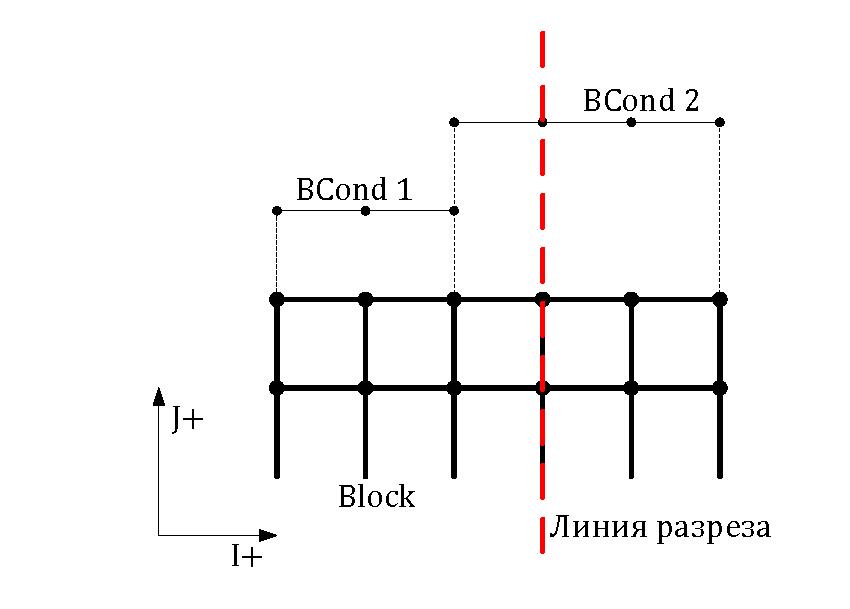
\includegraphics[width=0.45\textwidth]{./pics/text_2_withcut/cut-bcond.pdf}
&
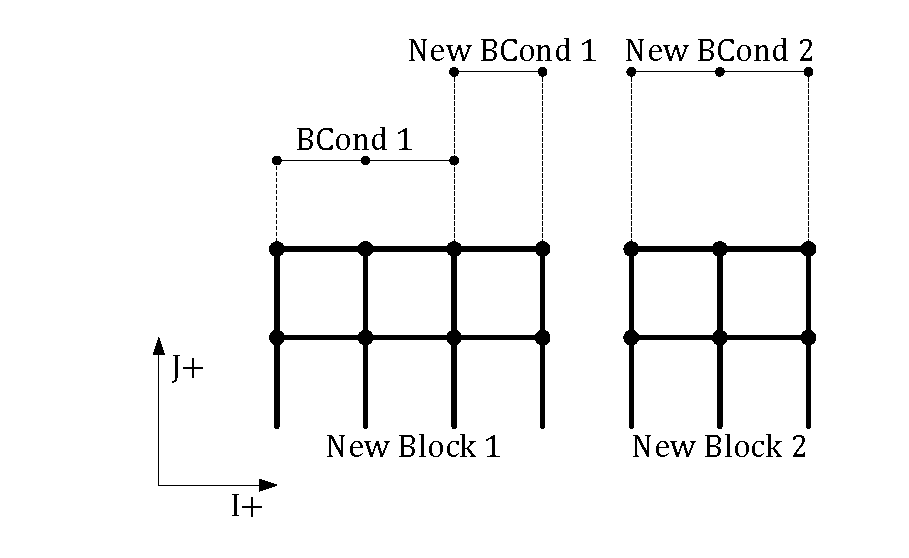
\includegraphics[width=0.45\textwidth]{./pics/text_2_withcut/cut-bcond2.pdf}
\end{tabular}
\singlespacing
\captionstyle{center}\caption{Дробление блока может спровоцировать дробление других объектов сетки.}
\label{fig:text_2_withcut_cut_bcond}
\end{figure}

Пусть блок Block должен быть разрезан по направлению $I+$ как показано на рис.~\ref{fig:text_2_withcut_cut_bcond} слева.
Пусть этот блок имеет граничные условия по направлению $J+$.
Тогда возможны два варианта.
Либо линия разреза не пересекает граничное условие, и тогда граничное условие целиком отходит одному из результирующих блоков (BCond 1).
Если же линия разреза проходит через граничное условие, то данное граничное условие также должно быть разделено, и его части отойдут двум результирующим блокам (рис.~\ref{fig:text_2_withcut_cut_bcond}, справа). Такая же ситуация может сложиться в отношении областей начальных условий.
В случае дробления интерфейсов могут быть более сложные ситуации дробления.

\subsubsection{Равномерное распределение блоков по вычислительным \\ процессам}

Для равномерного распределения блоков сетки по вычислительным процессам рассмотрим следующую задачу разделения множества весов на $m$ множеств.

Рассмотрим множество $X$ вещественных чисел $x_i \ge 0$ для $i \in N$, где $N = [1, n]$.
Рассмотрим также множество индексов $j \in M$, где $M = [1, m]$.
Будем говорить, что определено разбиение множества $X$ на $m$ множеств, если введена функция $\gamma(i): N \rightarrow M$.
Множество всех функций разбиения будем обозначать $\Gamma(N, M)$.
Веса результирующих множеств будем определять естественным образом для $j \in M$:
\begin{equation}
	X_j = \sum_{\substack{i \in N \\ \gamma(i) = j}}{x_i}
\end{equation}

Требуется найти такую функцию разбиения $\gamma \in \Gamma(N, M)$, чтобы минимизировать наиболее тяжелое из результирующих множеств $\max_{j \in M}{X_j}$.

Задача может быть расширена на случай распределения вычислительной нагрузки между вычислителями суперкомпьютера с разной производительностью.
При этом формулировка задачи меняется только в части приведения всех узлов к одному показателю с помощью весовых коэффициентов.

Коэффициентом приведения $\kappa(j)$ для $j \in M$ назовем такую положительную функцию $\kappa: M \rightarrow \mathbb{R}_{>0}$, что время выполнения нагрузки $\kappa(j)$ на узле $j$ не зависит от $j$.
Тогда в общем случае задача о равномерном разбиении множества весов на $m$ множеств с коэффициентами приведения $\kappa(j)$ для $j \in M$ формулируется следующим образом.
Требуется найти такую функцию разбиения $\gamma \in \Gamma(N, M)$, чтобы минимизировать наболее тяжелое из результирующих множеств с учетом коэффициентов приведения $\max_{j \in M}{ \frac{X_j}{\kappa(j)} }$.

Эта задача имеет практическое применение при распределении вычислительной нагрузки между вычислителями гетерогенного суперкомпьютера\label{term:cluster_getero2}.

Сформулированная задача является NP-полной, однако ее можно решить приближенно с помощью жадного алгоритма.
В жадном алгоритме будем последовательно обрабатывать все веса, начиная с наибольшего.
Каждый необработанный вес будем относить к наиболее легкому на текущий момент множеству весов.
Этот алгоритм является упрощенной версией алгоритма распределения вычислительной нагрузки между узлами гетерогенного вычислительного кластера, описанного в разделе \ref{sec:text_2_getero}.

Приведем оценку эффективности работы алгоритма.
Для удобства без ограничения общности будем считать, что изначальное множество весов упорядочено по убыванию.

Определим остаточный член $r_i$ для $i \in N$ по следующей формуле:
\begin{equation}
	r_i = \max{\left( x_i - \frac{1}{m} \sum_{p = i}^{n}{x_p}, 0 \right)}
\end{equation}

Тогда верно следующее утверждение

\begin{lemma}\label{lem:text_2_withcut_lem}
При использовании жадного алгоритма распределения весов между отдельными множествами отклонение наиболее тяжелого множества $\max_{j \in M}{X_j}$ от среднего значения веса множеств $\langle X \rangle$ не превышает максимальный остаточный член $r_i$, то есть
\begin{equation}
	\max_{j \in M}{X_j} - \langle X \rangle \le \max_{i \in N}{r_i}
\end{equation}
\end{lemma}
Пусть $X_k = \max_{j \in M}{X_j}$ -- наиболее тяжелое множество, а $x_t$ -- последний добавленный в него элемент.
Так как алгоритм является жадным, то до обработки веса $x_t$, $k$-е множество не превосходит по весу никакое другое множество, причем для любого $j \in M$ выполняется соотношение
\begin{equation}\label{lem:text_2_withcut_lem_single}
	X_k - x_t \le X_j - \chi_j,
\end{equation}	
	
где $\chi_j$ -- сумма весов, добавленных в $j$-е множество начиная с момента обработки веса $x_t$.
В частности, можно заметить, что $\chi_k = x_t$.

Почленно суммируя \eqref{lem:text_2_withcut_lem_single} по $j \in M$ получим соотношение
\begin{equation}
	m X_k - m x_t \le \sum_{j \in M}{X_j} - \sum_{p = t}^{n}{x_p},
\end{equation}

после деления которого на $m$ и переноса членов в нужные части неравенства, получим $X_k - \langle X \rangle \le r_t$ откуда следует утверждение леммы.
$\blacksquare$\\

Таким образом, для оценки эффективности описанного жадного алгоритма распределения весов по $m$ множествам достаточно проанализировать ряд остаточных членов, полученный из отсортированного массива распределяемых весов.

Задачу о равномерном распределении весов по результирующим множествам можно применить для равномерного распределения блоков блочно-структурированной расчетной сетки по вычислительным процессам суперкомпьютера в предположении, что все процессы равнозначны (не рассматривается случай гетерогенной системы).
В качестве веса блока нужно взять количество его ячеек.
Также заметим, что применительно к задаче распределения блоков расчетной сетки по вычислителям гомогенной системы оценка, полученная в лемме~\ref{lem:text_2_withcut_lem}, является оценкой показателя $D$ неравномерности распределения вычислительной нагрузки\label{term:decomp_neravn2}. 

Так как абсолютно равномерное распределение блоков по вычислительным процессам не всегда возможно, то нужно принять порог максимально допустимого отклонения количества ячеек одного процесса от среднего значения, при достижении которого распределение можно считать успешным.
Экспериментальным путем установлено, что порог максимального отклонения в 10\% является вполне достаточным для достижения эффективного распределения.
Если текущее распределение не удовлетворяет допустимому порогу отклонения количества ячеек процесса от среднего значения, то наиболее крупные блоки следует раздробить, после чего повторить оценку распределения.

\subsubsection{Результаты распределения блоков по процессам}

Рассмотренный алгоритм распределения вычислительной нагрузки блочно-структурированной сетки с дроблением блоков (применялось дробление наиболее крупных блоков пополам по наиболее протяженному направлению) между узлами гомогенной вычислительной системы был протестирован на различных расчетных сетках.
Ниже представлен результат тестирования на двух расчетных сетках.

Первая рассматриваемая сетка содержит 13 блоков, 80 интерфейсов, 148 граничных условий, 13 областей начальных условий и 5,75 млн ячеек, размер вычислительной окрестности равен 3.
Вторая рассматриваемая сетка содержит 300 блоков, 1796 интерфейсов, 1643 граничных условия, 300 областей начальных данных и 94,34 млн ячеек.
Размер вычислительной окрестности также равен 3.

Для этих сеток были проведены вычисления на 128 параллельных процессах.
Статистика распределения блоков по вычислительным процессам для двух различных вариантов: без использования дробления блоков и с использованием дроблений для достижения показателя неравномерности распределения распределения не более $D^{\%} = 10\%$ (см. рис.~\ref{fig:text_2_withcut_charts}).

\begin{figure}[ht]
\centering
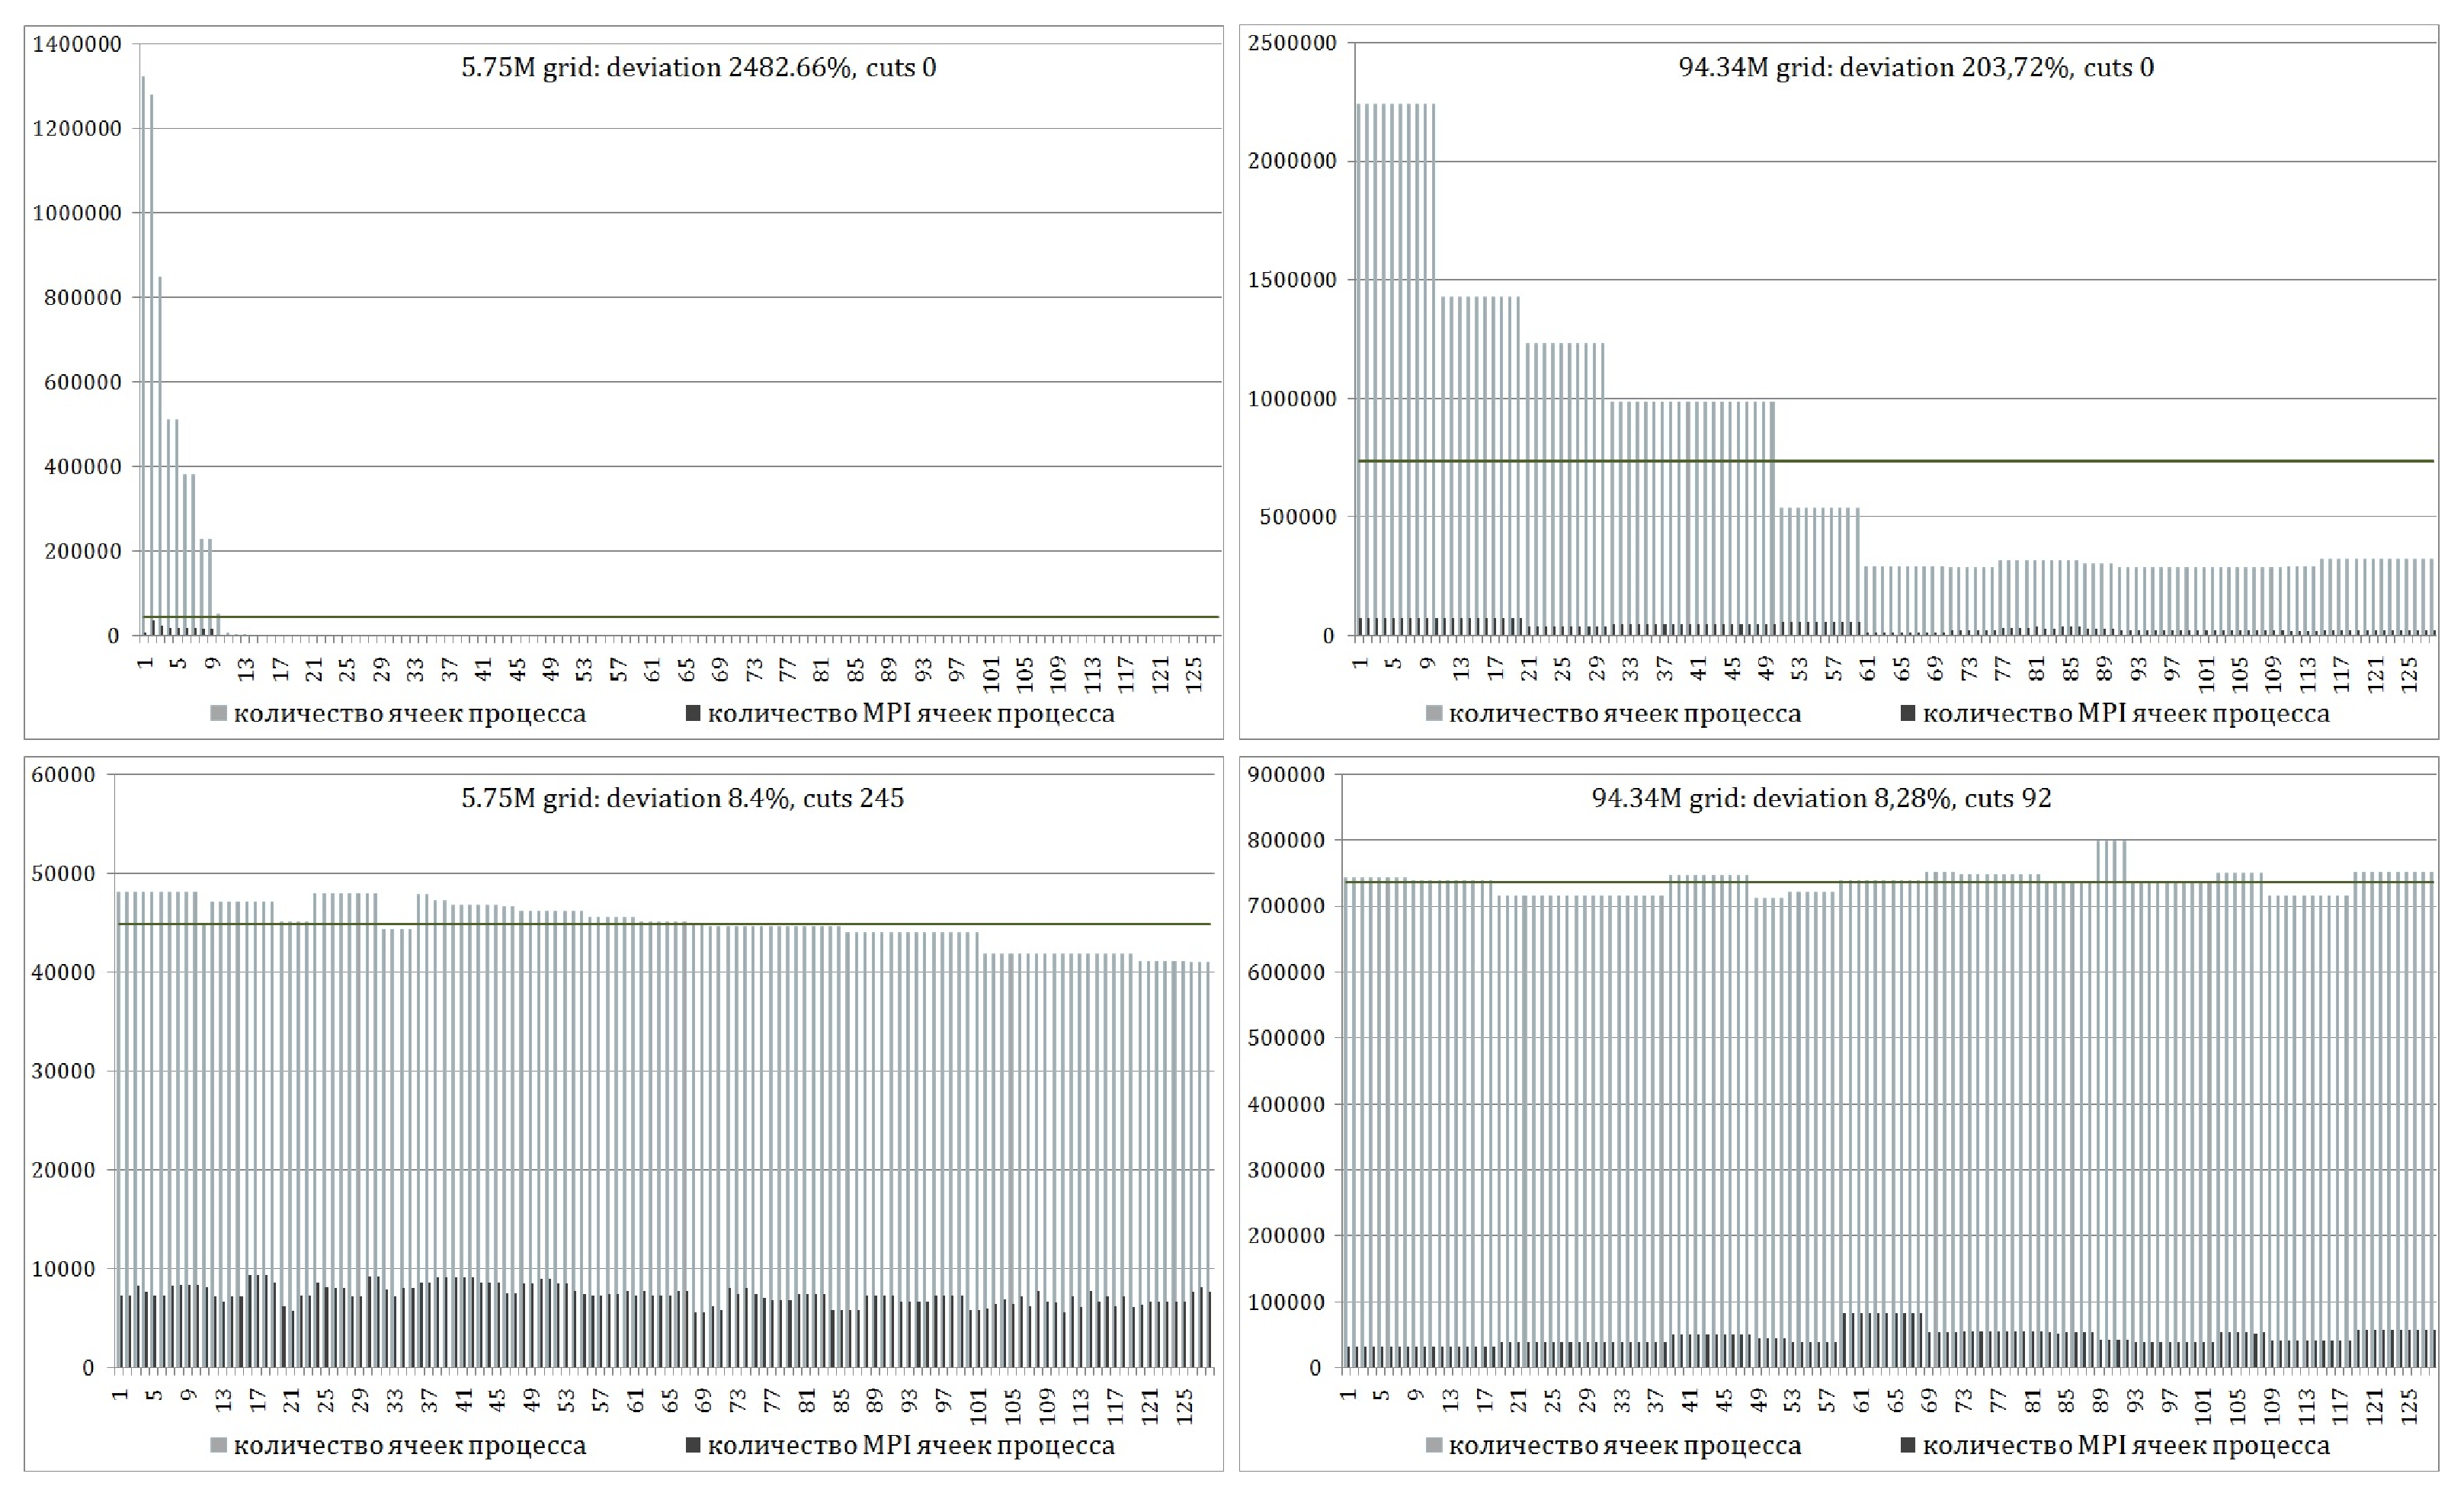
\includegraphics[width=1.0\textwidth]{./pics/text_2_withcut/withcut-charts.pdf}
\singlespacing
\captionstyle{center}\caption{Распределение блоков тестовых сеток (5,75 млн ячеек -- слева, 94,34 млн ячеек -- справа) без дробления (наверху) и с дроблением с допустимым отклонением $D^{\%} = 10\%$ (снизу).}
\label{fig:text_2_withcut_charts}
\end{figure}

Предложенный механизм распределения блоков блочно-структурированной сетки между узлами суперкомпьютерного кластера приводит к равномерной загрузке вычислительных ресурсов суперкомпьютерного кластера, что повышает эффективность его использования в расчетных задачах.
Часто применение такого подхода на большом количестве процессов приводит к кратному ускорению вычислений.
Особенно это актуально для сеток содержащих небольшое количество блоков или для сеток, имеющих ярко выраженные крупные блоки.

Негативным факторов применения дробления блоков является увеличение общего количества блоков и общего количества граничных ячеек, что приводит к увеличению объема данных межпроцессных обменов.

\subsubsection{Стратегии дробления блоков}

Рассмотрим различные стратегии дробления блоков при недостижении допустимого отклонения $D^{\%}$ при распределении блоков по процессам \cite{Bendersky2017Eff,Bendersky2018Block}.

Простейшая стратегия дробления блоков, использованная в предыдущем разделе, описывается следующим образом.
Сначала нужно применить жадный алгоритм распределения весов блоков по вычислительным узлам.
Если требуемое отклонение $D^{\%}$ наибольшего веса вычислительного узла от среднего значения достигнуто, то можно завершать работу.
В противном случае нужно разделить максимальный блок пополам по наиболее протяженному направлению, после чего произвести перераспределение.
Этот жадный алгоритм с дроблением пополам будем обозначать UG (от uniform greedy)\label{abbr:ug}.
Этот алгоритм всегда завершает работу, однако в отдельных случаях может выполнять необоснованно большое количество дроблений блоков, что приводит к возрастанию количества интерфейсных ячеек, а значит тормозит межпроцессные обмены между блоками сетки.

Для устранения крупных блоков без лишних дроблений предлагается механизм минимизации количества разрезов блоков.
Прежде всего определим, на какие части может быть разрезан конкретный блок, имеющий размеры $IS$, $JS$, $KS$ и содержащий соответственно $IS \times JS \times KS$ ячеек.

На возможные разрезы блока накладываются следующие ограничения.
Так как блок может быть разрезан только по границам ячеек, то размеры получившихся новых блоков будут кратны одному из значений $IS \times JS$, $IS \times KS$, или $JS \times KS$.
На самом деле, целесообразно выполнять разрезы только по наиболее протяженному направлению (пусть это будет $IS$, для каждого блока это направление будет свое), так как это приводит к минимизации количества интерфейсных ячеек.
Для запрета появления слишком тонких блоков по одному из измерений запрещается выполнять разрезы блока слишком близко к границе.
Для этого вводится специальный параметр $m$ (margin), по которому разрешается деление блока только в сегменте $[m, IS - m]$.
Вводится еще одно ограничение, не позволяющее производить слишком мелкие блоки (задается наименьшее допустимое количество ячеек в результирующем блоке, при котором разрешено дробление).

Алгоритм распределения блоков по вычислительным узлам с минимизацией количества разрезов (в дальнейшем будем обозначать его MCC, от minimal cuts count\label{abbr:mcc}) будем описывать в следующем виде:

1) Определить среднее ожидаемое количество ячеек, которое должно приходиться на один вычислительный узел, будем обозначать эту величину $mid$.
Она равна общему количеству ячеек сетки, деленному на количество вычислительных узлов $proc$.

2) Определить максимально допустимый вес вычислительно узла на текущий момент (будем обозначать через $max$).
Изначально $max$ берется равным $mid$.
Однако если в процессе распределения вес какого-либо вычислительного узла превысил $mid$, то величина $max$ принимает значение веса этого узла.
Таким образом $max$ определяется как максимум из величины $mid$ и всех весов вычислительных узлов.

3) Определить множество всех блоков, которые еще не распределены ни на один вычислительный узел.
Если это множество пусто, то алгоритм заканчивает работу.

4) Попробовать найти из рассматриваемого множества блоков такой блок, который можно распределить на один из вычислительных узлов так, чтобы вес этого узла не превысил $max$.
Если таких блоков несколько, то нужно взять такой блок, который максимально приближает вес соответствующего вычислительного узла к отметке $max$.
Если это удалось сделать, то распределить найденный блок на вычислительный узел и перейти к пункту 3.

5) Определить множество допустимых разрезов всех не распределенных на текущий момент блоков.
Каждый потенциальный разрез делит блок на две части.
Определить множество таких потенциальных результирующих блоков и из этих потенциальных блоков выбрать блок веса $w$ и вычислительный узел веса $W$ такие, что $W + w \le max$ и величина $max - (W + w)$ минимальна.
Если такой пары блок-узел не найдено, то найти такую пару, что $W + w > max$ и величина $(W + w) - max$ минимальна.
Такая пара найдется всегда.
После этого выполнить необходимый разрез для получения найденного блока и распределить его на соответствующий вычислительный узел, после чего перейти к пункту 2.

Кроме описанных действий приведенный алгоритм содержит ряд эвристик, не позволяющих проявляться негативным эффектам при возникновении сложных краевых случаев (например, неконтролируемый рост величины $max$). 
Таким образом, описанный  алгоритм на каждом шаге пытается выполнить такой разрез блока, чтобы максимально приблизить вес некоторого вычислительного узла к ожидаемой в среднем величине загрузки.

Для тестирования и оценки эффективности описанных выше методов распределения блоков блочно-структурированной сетки между узлами суперкомпьютерного кластера использовались три разные сетки, отличающиеся по количеству блоков: test (13 блоков, 5,8 млн ячеек), train (30 блоков, 10,7 млн ячеек), ref (136 блоков, 8,5 млн ячеек).

В качестве целевого вычислительного ресурса брался гомогенный вычислительный кластер\label{term:cluster_gomo2}, состоящий из 64 узлов.
Величина $m$, характеризующая минимальное расстояние разреза от границы блока, бралась равной 5.
На рис.~\ref{fig:text_2_withcut_2_merged_pic} представлены данные применения алгоритмов UG и MCC к каждой из приведенных расчетных сеток.
Описание данных на графиках: $mid$ -- средний ожидаемый вес вычислительного узла, $dev$ -- отклонение веса наиболее тяжелого узла от $mid$, $proc$ -- количество вычислительных узлов, $cuts$ -- количество выполненных разрезов, iface cells и cross cells -- доля интерфейсных и MPI ячеек среди всех ячеек сетки.

На каждом графике на рис.~\ref{fig:text_2_withcut_2_merged_pic}, представлена гистограмма распределения блоков расчетной сетки по вычислительным узлам.
Каждый столбец гистограммы соответствует одному вычислительному узлу.
Высота столбца -- вес соответствующего вычислительного узла.
Если к вычислительному узлу отнесены несколько блоков расчетной сетки, то соответствующий столбец гистограммы разделен на несколько частей, размеры которых отражают веса блоков, также эти части раскрашены в шахматном порядке для повышения наглядности.

\begin{figure}[ht]
\centering
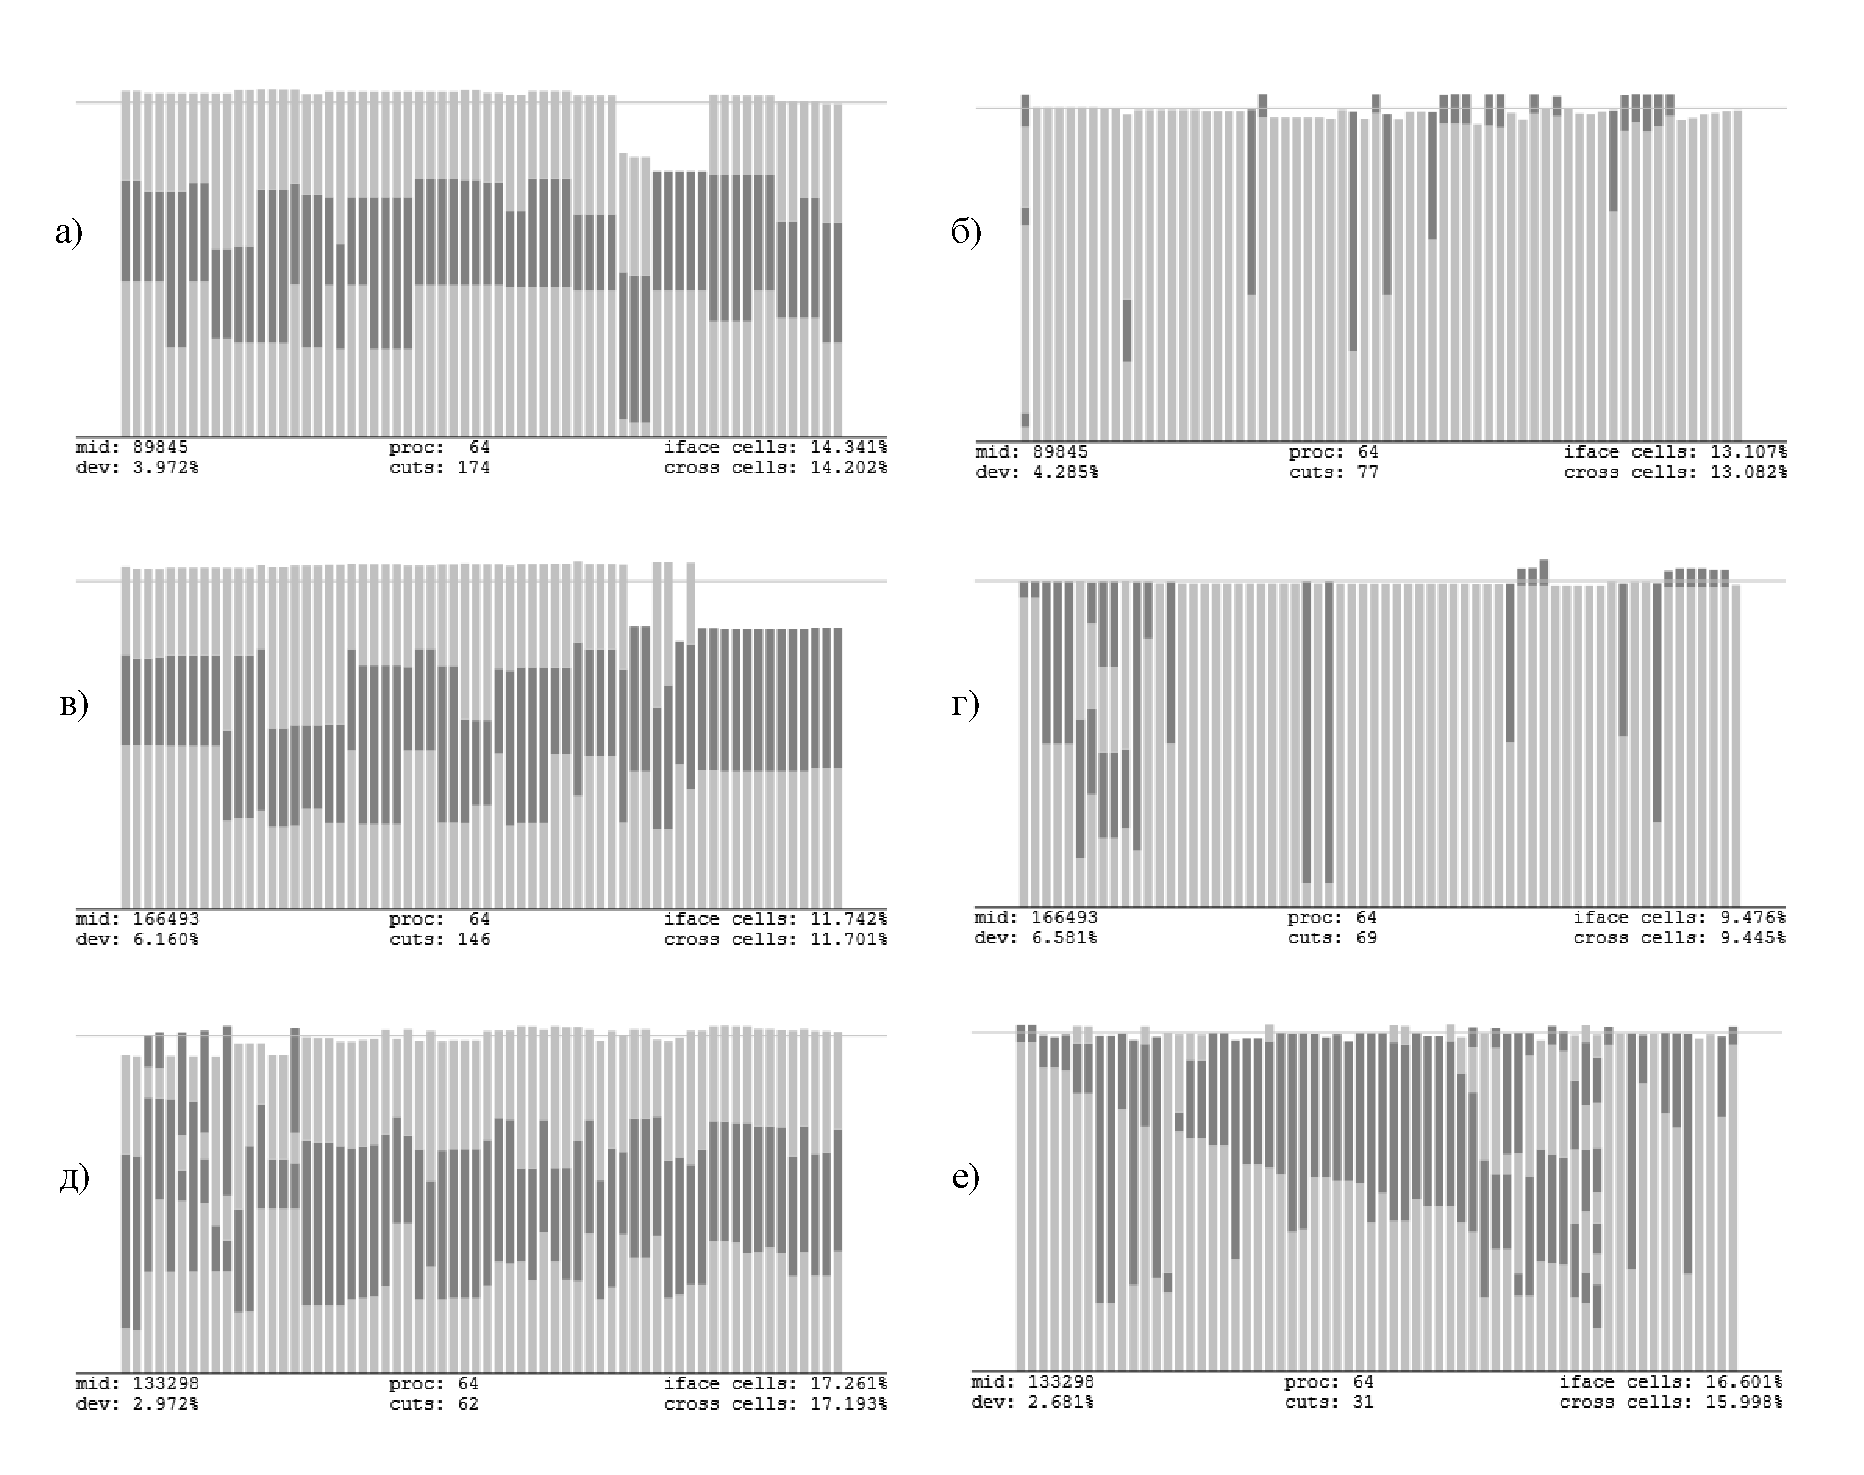
\includegraphics[width=1.0\textwidth]{./pics/text_2_withcut/2-merged-pic.pdf}
\singlespacing
\captionstyle{center}\caption{Гистограммы распределения блоков расчетной сетки по вычислительным узлам суперкомпьютера для сеток test (а, б), train (в, г), ref (д, е) с помощью алгоритмов UG (а, в, д) и MCC (б, г. е).}
\label{fig:text_2_withcut_2_merged_pic}
\end{figure}

Результаты сравнения эффективности методов UG и MCC распределения вычислительной нагрузки между узлами суперкомпьютера показывают, что использование метода MCC оправдано, так как с его помощью можно добиться распределения не худшего качества (а зачастую и лучшего), чем при использовании UG.
При этом MCC позволяет существенно сократить количество разрезов блоков сетки для достижения требуемого результата.
Также использование MCC приводит к сокращению количества MPI ячеек в сетке, что положительно сказывается на скорости межпроцессных обменов данными.
Особенно явно достоинства метода MCC проявляются на сетках с относительно небольшим количеством блоков и наличием ярко выраженных крупных блоков.

Для анализа эффективности метода распределения вычислительной нагрузки для блочно-структурированной сетки с дроблением узлов были произведены расчетны на модельном воздухозаборном устройстве высокоскоростного летательного аппарата, описанные в \cite{Bendersky2017Eff}.
Для этого объекта проводились численные расчеты на суперкомпьютере с использованием RANS/ILES метода.
Для проведения численных расчетов использовалась блочная расчетная сетка, содержащая 172 блока, 848 интерфейсов, 323 граничных условия, 12,8 миллионов ячеек.
Для распределения вычислительной нагрузки для этой сетки использовался алгоритм MCC с дроблением блоков.
В качестве вычислительного поля использовались узлы суперкомпьютера МВС-10П, каждый вычислительный узел содержит по 2 микропроцессора Intel Xeon E5-2697v3 (Haswell).
Были выполнены запуски расчетов в двух конфигурациях: с запуском двух MPI процессов на каждом процессоре и с запуском четырех MPI процессов на каждом процессоре.
Количество вычислительных узлов варьировалось от 1 до 18.
В качестве эталонного запуска, относительно которого считались ускорения, был выбран запуск на одном узле с двумя MPI процессами на каждом процессоре. 

\begin{figure}[ht]
\centering
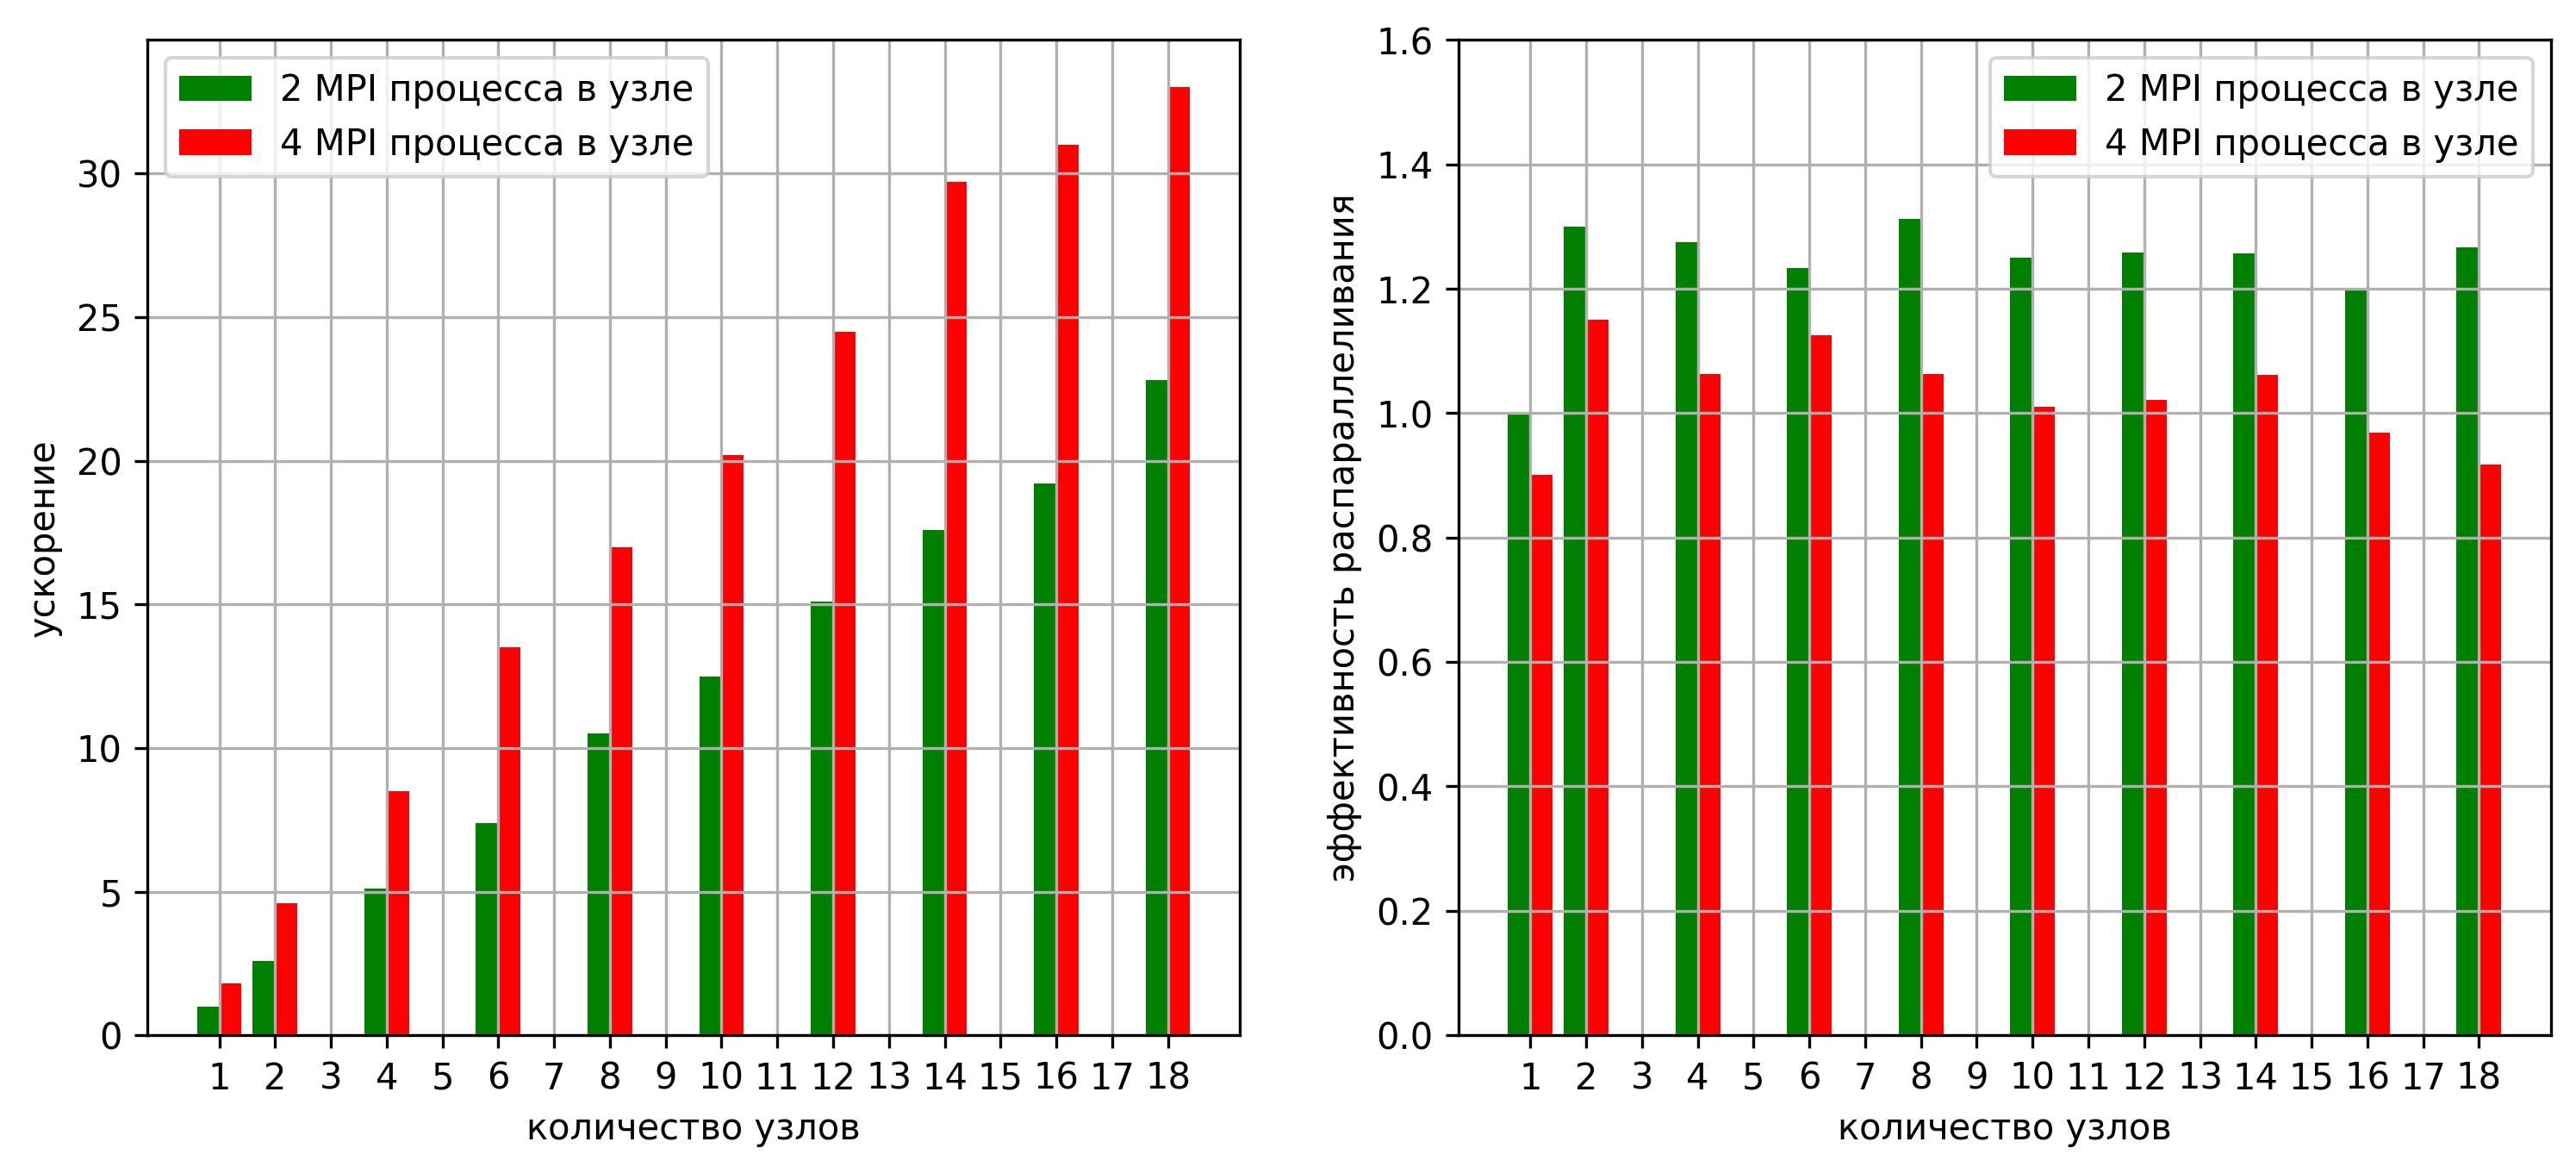
\includegraphics[width=1.0\textwidth]{./pics/text_2_withcut/scaling2.png}
\singlespacing
\captionstyle{center}\caption{Ускорение запусков и эффективность распараллеливания на различном числе узлов относительно эталонного запуска при проведении газодинамических расчетов на модельном входном устройстве воздухозаборника на суперкомпьютере с использованием RANS/ILES метода.}
\label{fig:text_2_withcut_scaling2}
\end{figure}

Из данных, приведенных на рис.~\ref{fig:text_2_withcut_scaling2}, можно видеть сверхлинейное ускорение при увеличении количества расчетных узлов.
Так, при использовании 18 узлов с двумя MPI процессами на каждом процессоре было достигнуто 23-хкратное ускорение относительно эталонного запуска.
Такое сверхлинейное ускорение объясняется как равномерностью распределения вычислительной нагрузки между узлами суперкомпьютерного кластера, так и снижением интенсивности и повышением локальности обращений в память при увеличении количества вычислительных узлов.
При использовании 4 MPI процессов на каждом процессоре эффективность счета увеличивается, при этом линейное масштабирование сохраняется.

\subsubsection{Масштабирование вычислений с разными порогами \\ отклонения}

Для анализа эффективности распределения блоков по вычислительным процессам с использованием дробления блоков был поставлен эксперимент по выполнению расчетов методом RANS/ILES на блочно-структурированной расчетной сетке, содержащей 10,7 млн ячеек \cite{Savin2019RANS}.

Перед вычислениями выполнялась подготовка расчетной сетки для 16, 32 и 64 процессов путем распределения вычислительной нагрузки с дроблением блоков сетки с помощью алгоритма UG, описанного в предыдущем разделе.
При подготовке расчетной сетки использовалось допустимое отклонение $D^{\%} = 10\%$, для подготовки вычислений на 64 процессах также использовалось допустимое отклонение $D^{\%} = 1\%$.

\begin{table}[!ht]
\centering
\singlespacing
\captionstyle{center}\caption{Характеристики используемых расчетных сеток.}
\bigskip
\label{tbl:text_2_withcut}
\begin{tabular}{ | c | c | c | c | c | }
  \hline
  Описание & Блоки & Интерфейсы & Граничые условия \\ \hline\hline
  исходная сетка & 30 & 152 & 204 \\ \hline\hline
  \makecell{подготовленная сетка \\ 16 проц., 10\% откл.} & 39 & 224 & 218 \\ \hline
  \makecell{подготовленная сетка \\ 32 проц., 10\% откл.} & 54 & 340 & 248 \\ \hline
  \makecell{подготовленная сетка \\ 64 проц., 10\% откл.} & 170 & 982 & 429 \\ \hline\hline
  \makecell{подготовленная сетка \\ 64 проц., 1\% откл.} & 383 & 2356 & 682 \\ \hline
\end{tabular}
\end{table}

\begin{figure}[ht]
\centering
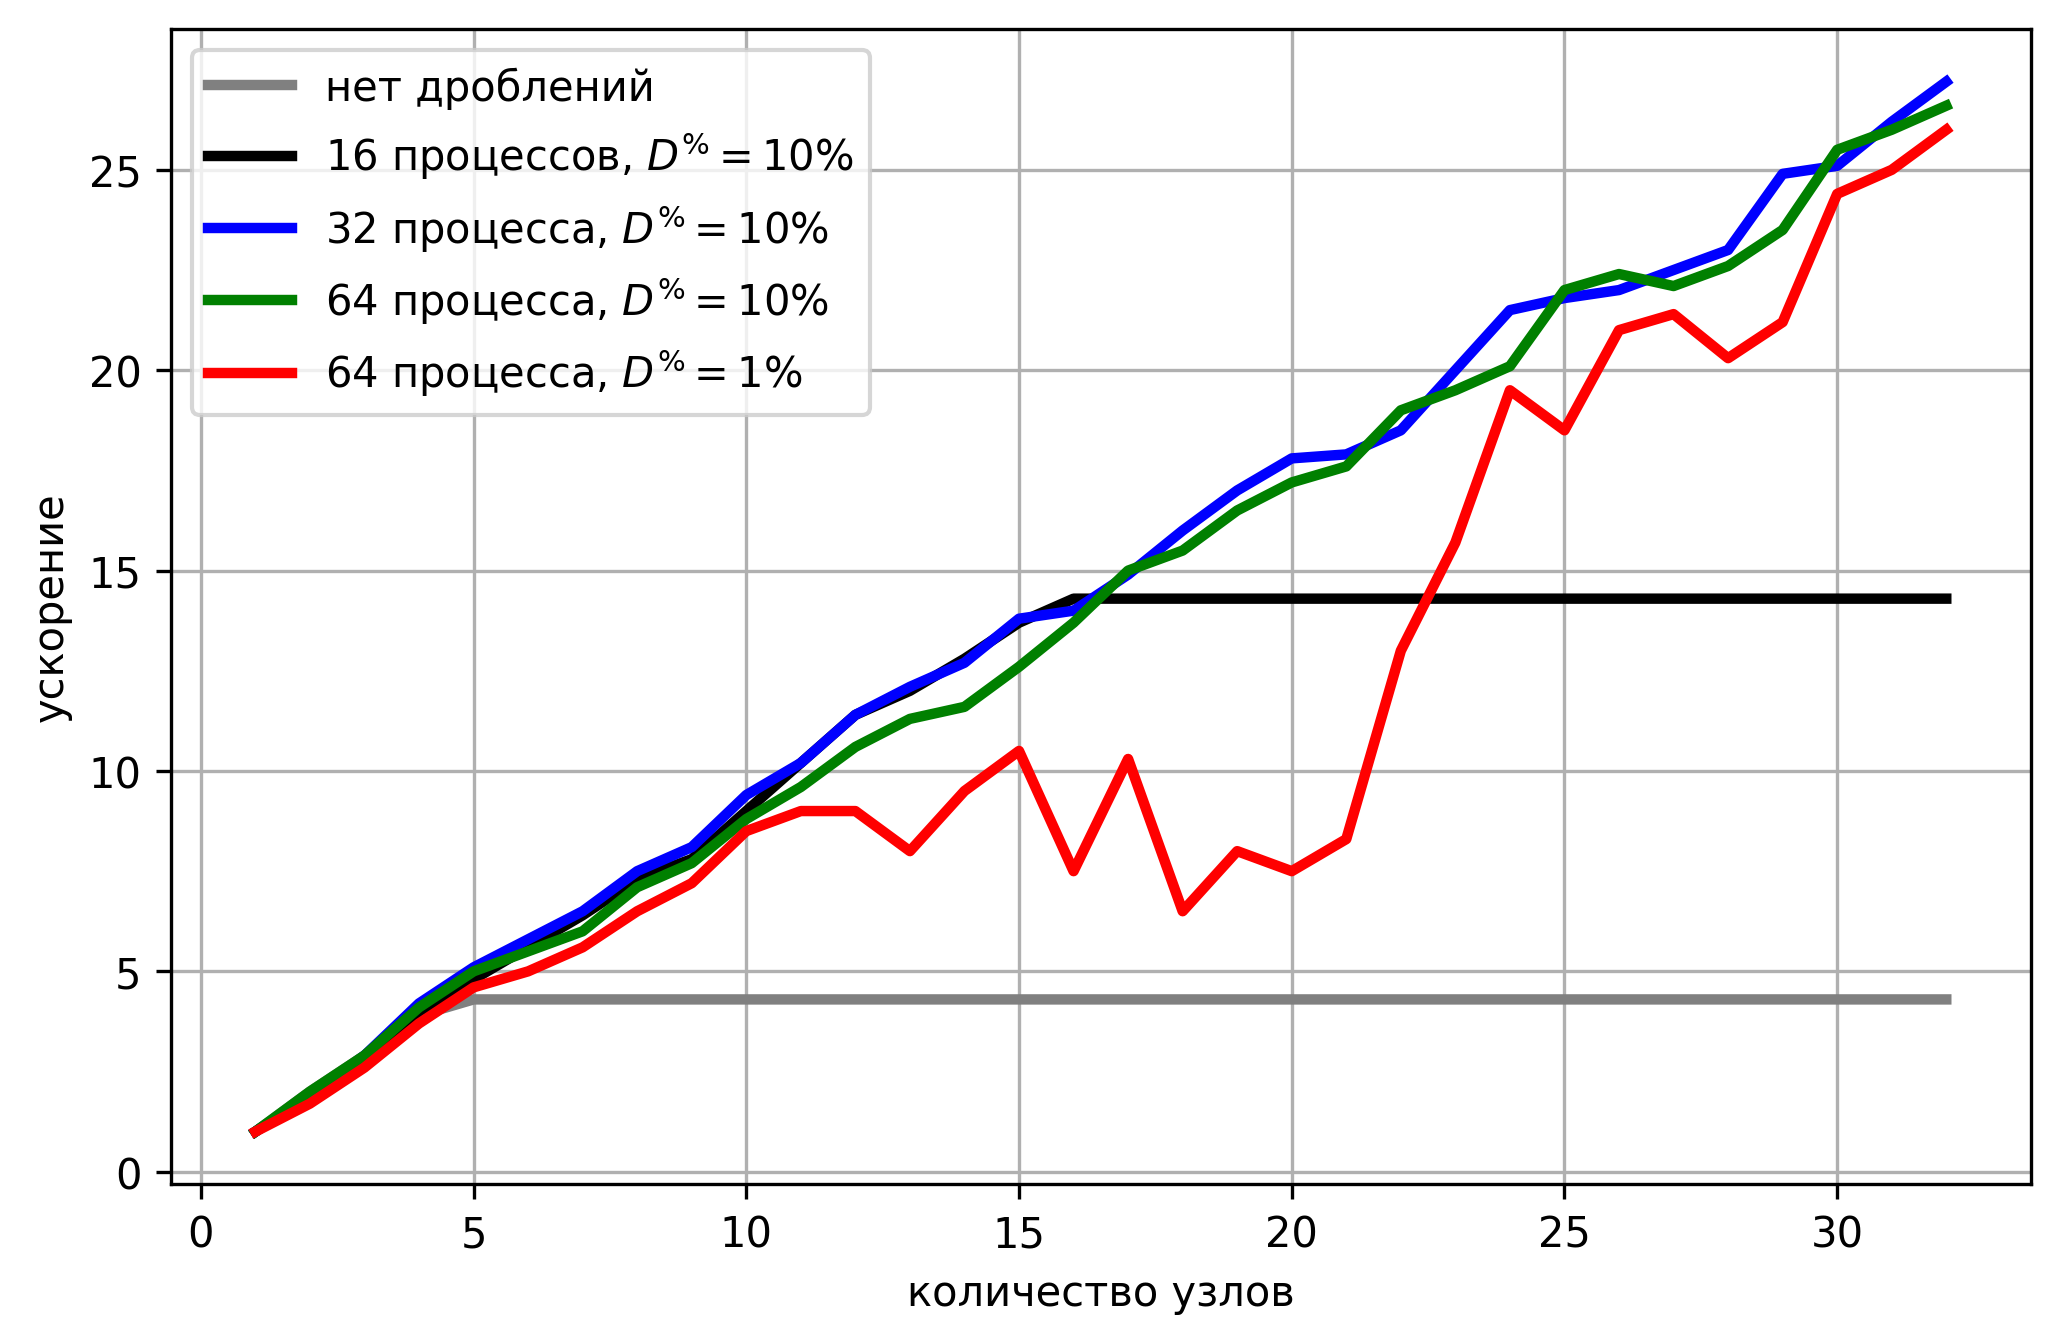
\includegraphics[width=1.0\textwidth]{./pics/text_2_withcut/scaling3.png}
\singlespacing
\captionstyle{center}\caption{Масштабирование вычислений при различных параметрах дробления сетки на 1-32 микропроцессорах Intel Xeon Phi Knights Landing 7290.}
\label{fig:text_2_withcut_scaling3}
\end{figure}

На рис.~\ref{fig:text_2_withcut_scaling3} представлены результаты численных экспериментов на сегменте суперкомпьютера, состоящем из узлов, каждый из которых содержит по одному микропроцессору Intel Xeon Phi Knights Landing 7290.
При проведении расчетов на каждом узле запускался один MPI процесс.
Количество узлов менялось от 1 до 32.
Проанализируем графики ускорения вычислений, представленные на рис.~\ref{fig:text_2_withcut_scaling3}.

Для вычислений на неподготовленной сетке (соответствует графику "нет дроблений") наблюдается ускорение для количества процессов до 5.
Далее ускорение остается на одной и той же отметке (около 4,3) и не меняется при дальнейшем увеличении количества узлов.
Это связано с наличием крупного блока, который мешает равномерному распределению вычислительной нагрузки.

При подготовке сетки для выполнения на 16 процессах (черный график) ускорение также останавливается, но на более высокой отметке (в районе 14,0).
Это также связано с наличием крупного блока, но его размер меньше, чем в случае отказа от дроблений (наиболее крупный блок был раздроблен, что привело к эффективному распределению вычислительной нагрузки для 16 процессов, однако для большего количества процессов размер этого блока препятствует равномерному распределению блоков по процессам).

При подготовке сетки для выполнения на 32 и 64 процессах с допустимым отклонением $D^{\%} = 10\%$ (синий и зеленый графики соответственно) получаем примерно одинаковое возрастание ускорения вычислений с ростом количества узлов.
Это говорит о том, что при подготовка сетки для большего количества процессов, чем реально будет использоваться для запусков, избыточно.

При подготовке сетки для выполнения на 64 процессах с допустимым отклонением $D^{\%} = 1\%$ (красный график) наблюдается сильная просадка по ускорению при использовании количества узлов от 10 до 25.
Это связано с сильным возрастанием количества MPI ячеек\label{term:cell_block_mpi2}, что приводит к увеличению доли межпроцессных обменов.

Из графиков, приведенных на рис.~\ref{fig:text_2_withcut_scaling3}, можно сделать вывод, что при использовании распределения вычислительной нагрузки с дроблением блоков целесообразно предерживаться двух эвристических правил.
Во-первых, подготовку расчетной сетки не следует производить для количества процессов, больше того, которое реально будет использоваться при запусках.
Во-вторых, не стоит выбирать слишком низкий показатель допустимого отклонения $D^{\%}$, так как в случае слишком низкого значения этого показателя равномерность распределения вычислительной нагрузки будет нивелирована возрастанием объема межпроцессных обменов.

%---------------------------------------------------------------------------------------------------
% 4.3 - декомпозиция поверхностной сетки со сглаживанием границ

\subsection{Декопмозиция поверхностной сетки со сглаживанием границ}

% Декомпозиция поверхностной сетки.
\subsubsection{Декомпозиция поверхностной неструктурированной расчетной сетки}

В этом разделе будем рассматривать подходы к декомпозиции неструктурированной поверхностной расчетной сетки с треугольными ячейками\label{term:unstruct_surf_calc_mesh3} \cite{Rybakov2020Decomp}.
В отличие от блочно-структурированных сеток\label{term:mesh_block_struct4} у рассматриваемой неструктурированной сетки ячейки не объединяются в блоки, а являются независимыми объектами проведения расчетов.
Для неструктурированных поверхностных сеток будем считать, что вычислительная окрестность\label{term:cell_calc_template2} каждой ячейки будет влючать кроме нее самом только три смежные ячейки (граничащие с рассматривамой по каждому из трех ребер).

\subsubsection{Описание методов декомпозиции}

Будем рассматривать алгоритмы декомпозиции на примере тестовой трехмерной поверхностной сетки (wing), состоящей из ячеек-треугольников.
Сетка представляет собой профиль крыла летательного аппарата и содержит порядка $n = 2 \cdot 10^4$ ячеек.
Внешний вид тестовой расчетной сетки представлен на рис.~\ref{fig:text_2_decompsurf_wing_grid}.
Этот трехмерный профиль был сгенерирован из двумерного профиля NACA 0012.

\begin{figure}[ht]
\centering
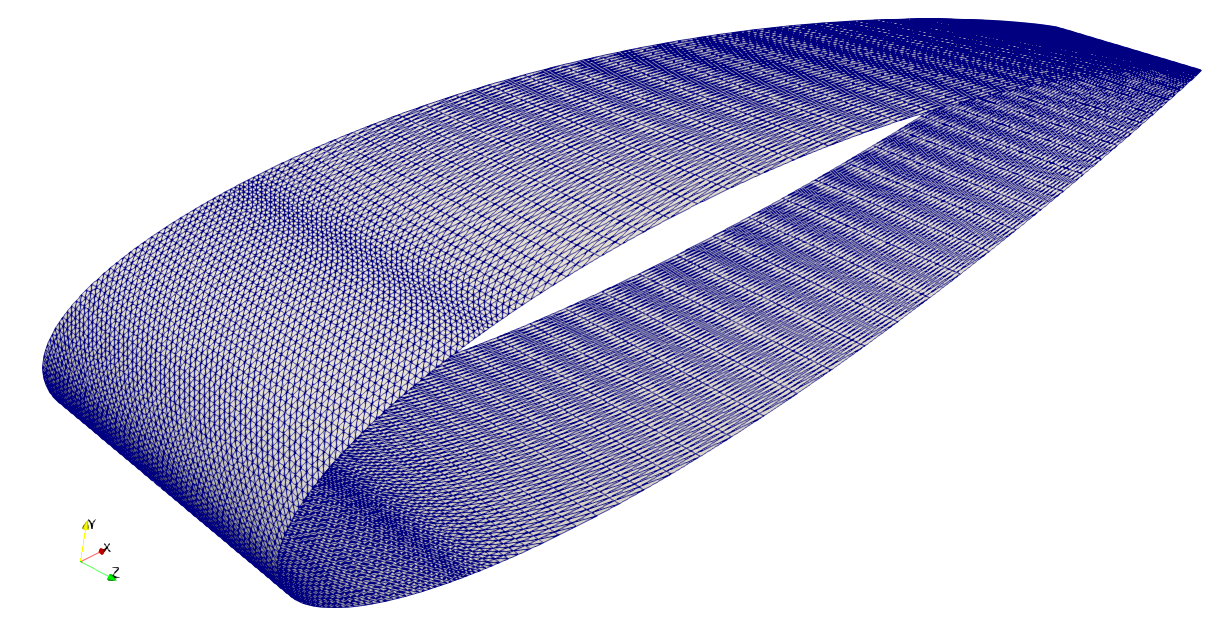
\includegraphics[width=0.5\textwidth]{./pics/text_2_decompsurf/wing_grid.png}
\singlespacing
\captionstyle{center}\caption{Внешний вид расчетной сетки wing, используемой для тестирования алгоритмов декомпозиции.}
\label{fig:text_2_decompsurf_wing_grid}
\end{figure}

\begin{figure}[ht]
\centering
\begin{tabular}{ll}
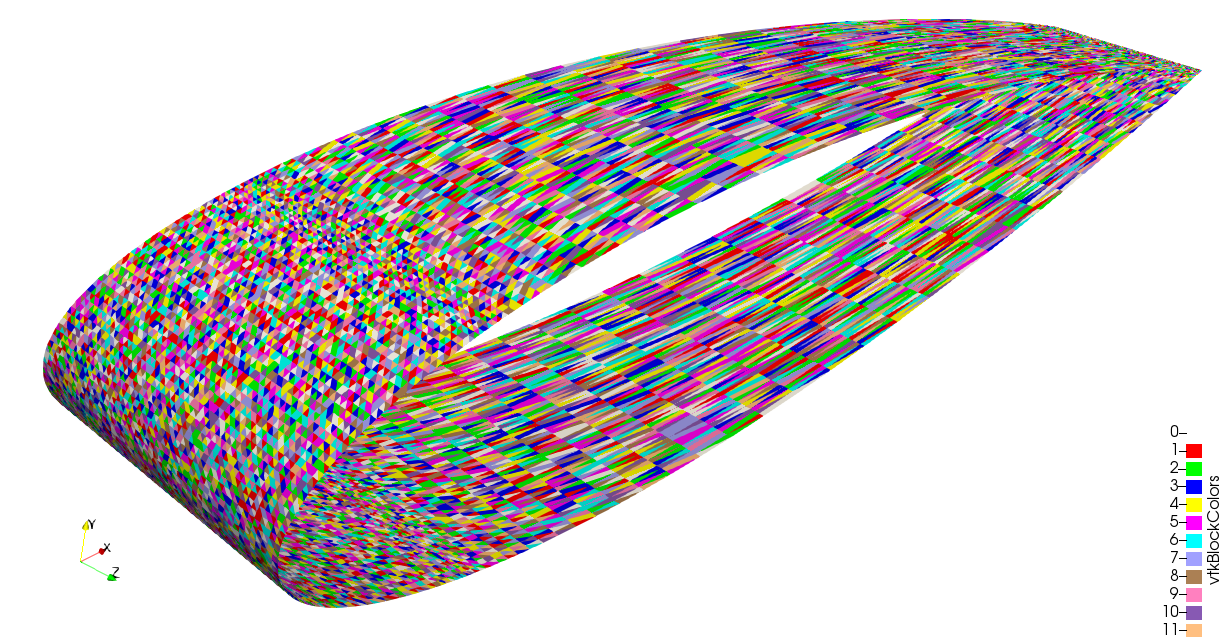
\includegraphics[width=0.45\textwidth]{./pics/text_2_decompsurf/wing_random_32.png}
&
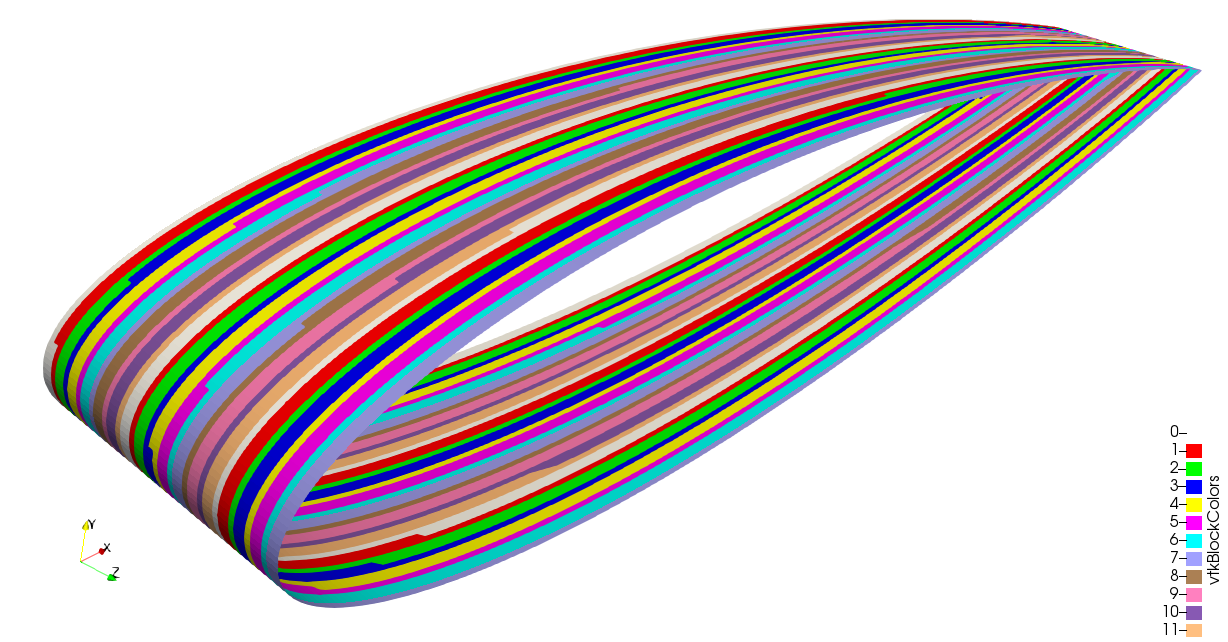
\includegraphics[width=0.45\textwidth]{./pics/text_2_decompsurf/wing_linear_32.png}
\\
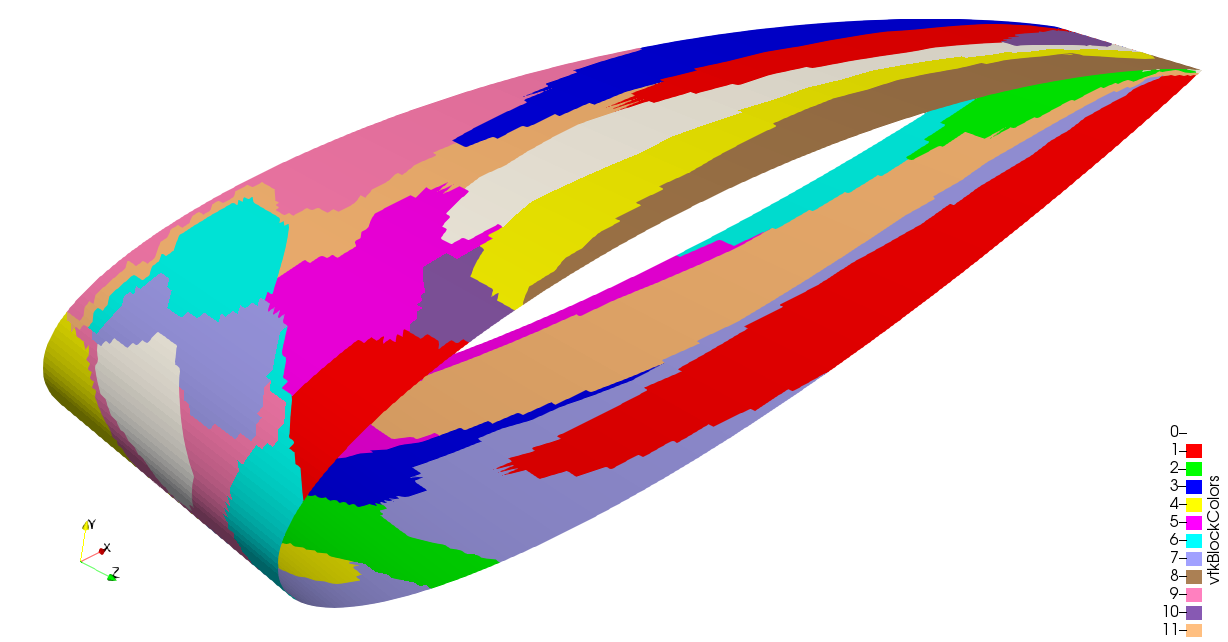
\includegraphics[width=0.45\textwidth]{./pics/text_2_decompsurf/wing_rgrow_32.png}
&
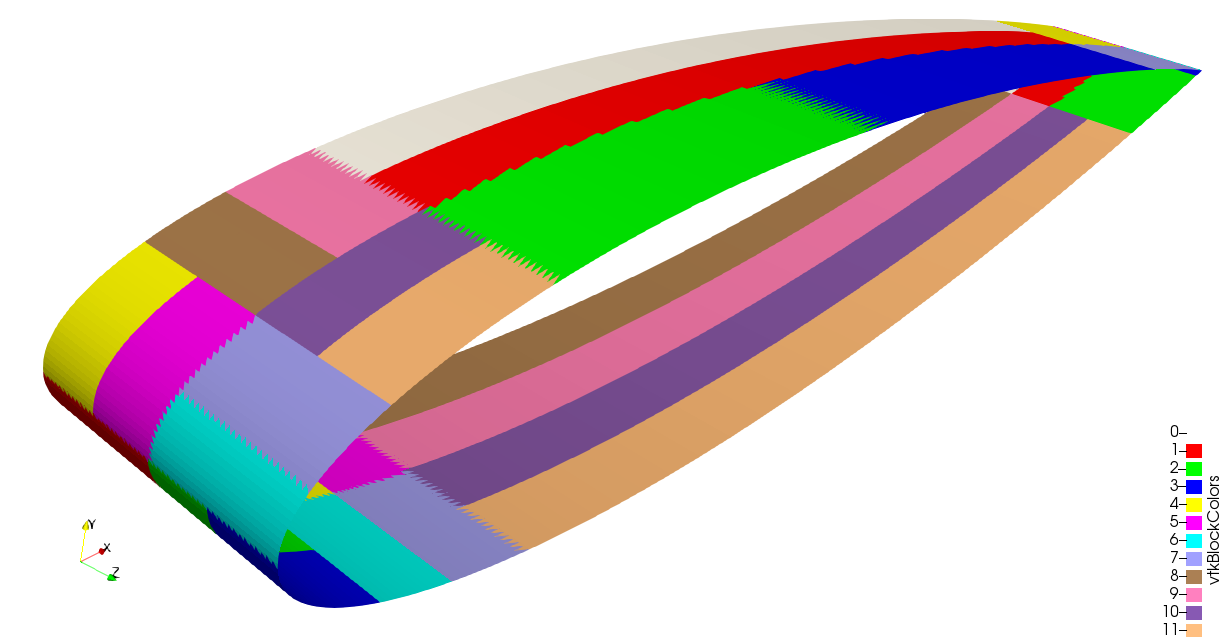
\includegraphics[width=0.45\textwidth]{./pics/text_2_decompsurf/wing_hierarchical_32.png}
\end{tabular}
\singlespacing
\captionstyle{center}\caption{Результат декомпозиции расчетной сетки на 32 домена. Сверху вниз слева направо -- случайное распределение, линейное распределение, наращивание доменов и иерархическое дробление\label{term:alg_decomp_hierarch}.}
\label{fig:text_2_decompsurf_4}
\end{figure}

В качестве первого и самого простого алгоритма декомпозиции рассмотрим алгоритм случайного распределения\label{term:alg_decomp_random} ячеек расчетной сетки по доменам.
Результат применения этого алгоритма к тестовой сетке показан на рис.~\ref{fig:text_2_decompsurf_4} сверху слева.
Алгоритм случайного распределения имеет достаточно низкое значение по критерию $D$\label{term:decomp_neravn3}, то есть распределение ячеек по доменам равномерное, однако при случайном распределении практически все ребра с высокой долей вероятности являются междоменными\label{term:edge_cross2}, что порождает огромный объем данных, которыми нужно обмениваться при синхронизации вычислений.
Также следует отменить, что при случайном распределении ячеек по доменам любые два домена\label{term:domain2} оказываются соседними, граф связности доменов является полным.
Таким образом, каждый домен должен обмениваться данными со всеми остальными доменами по достаточно протяженным границам.
Также алгоритм становится совершенно непригодным, когда возникает необходимость создания теневых слоев\label{term:block_shadow_layer2} глубиной больше единицы.
Использование таких буферных зон может потребоваться для реализации численных методов повышенной точности.

\begin{figure}[ht]
\centering
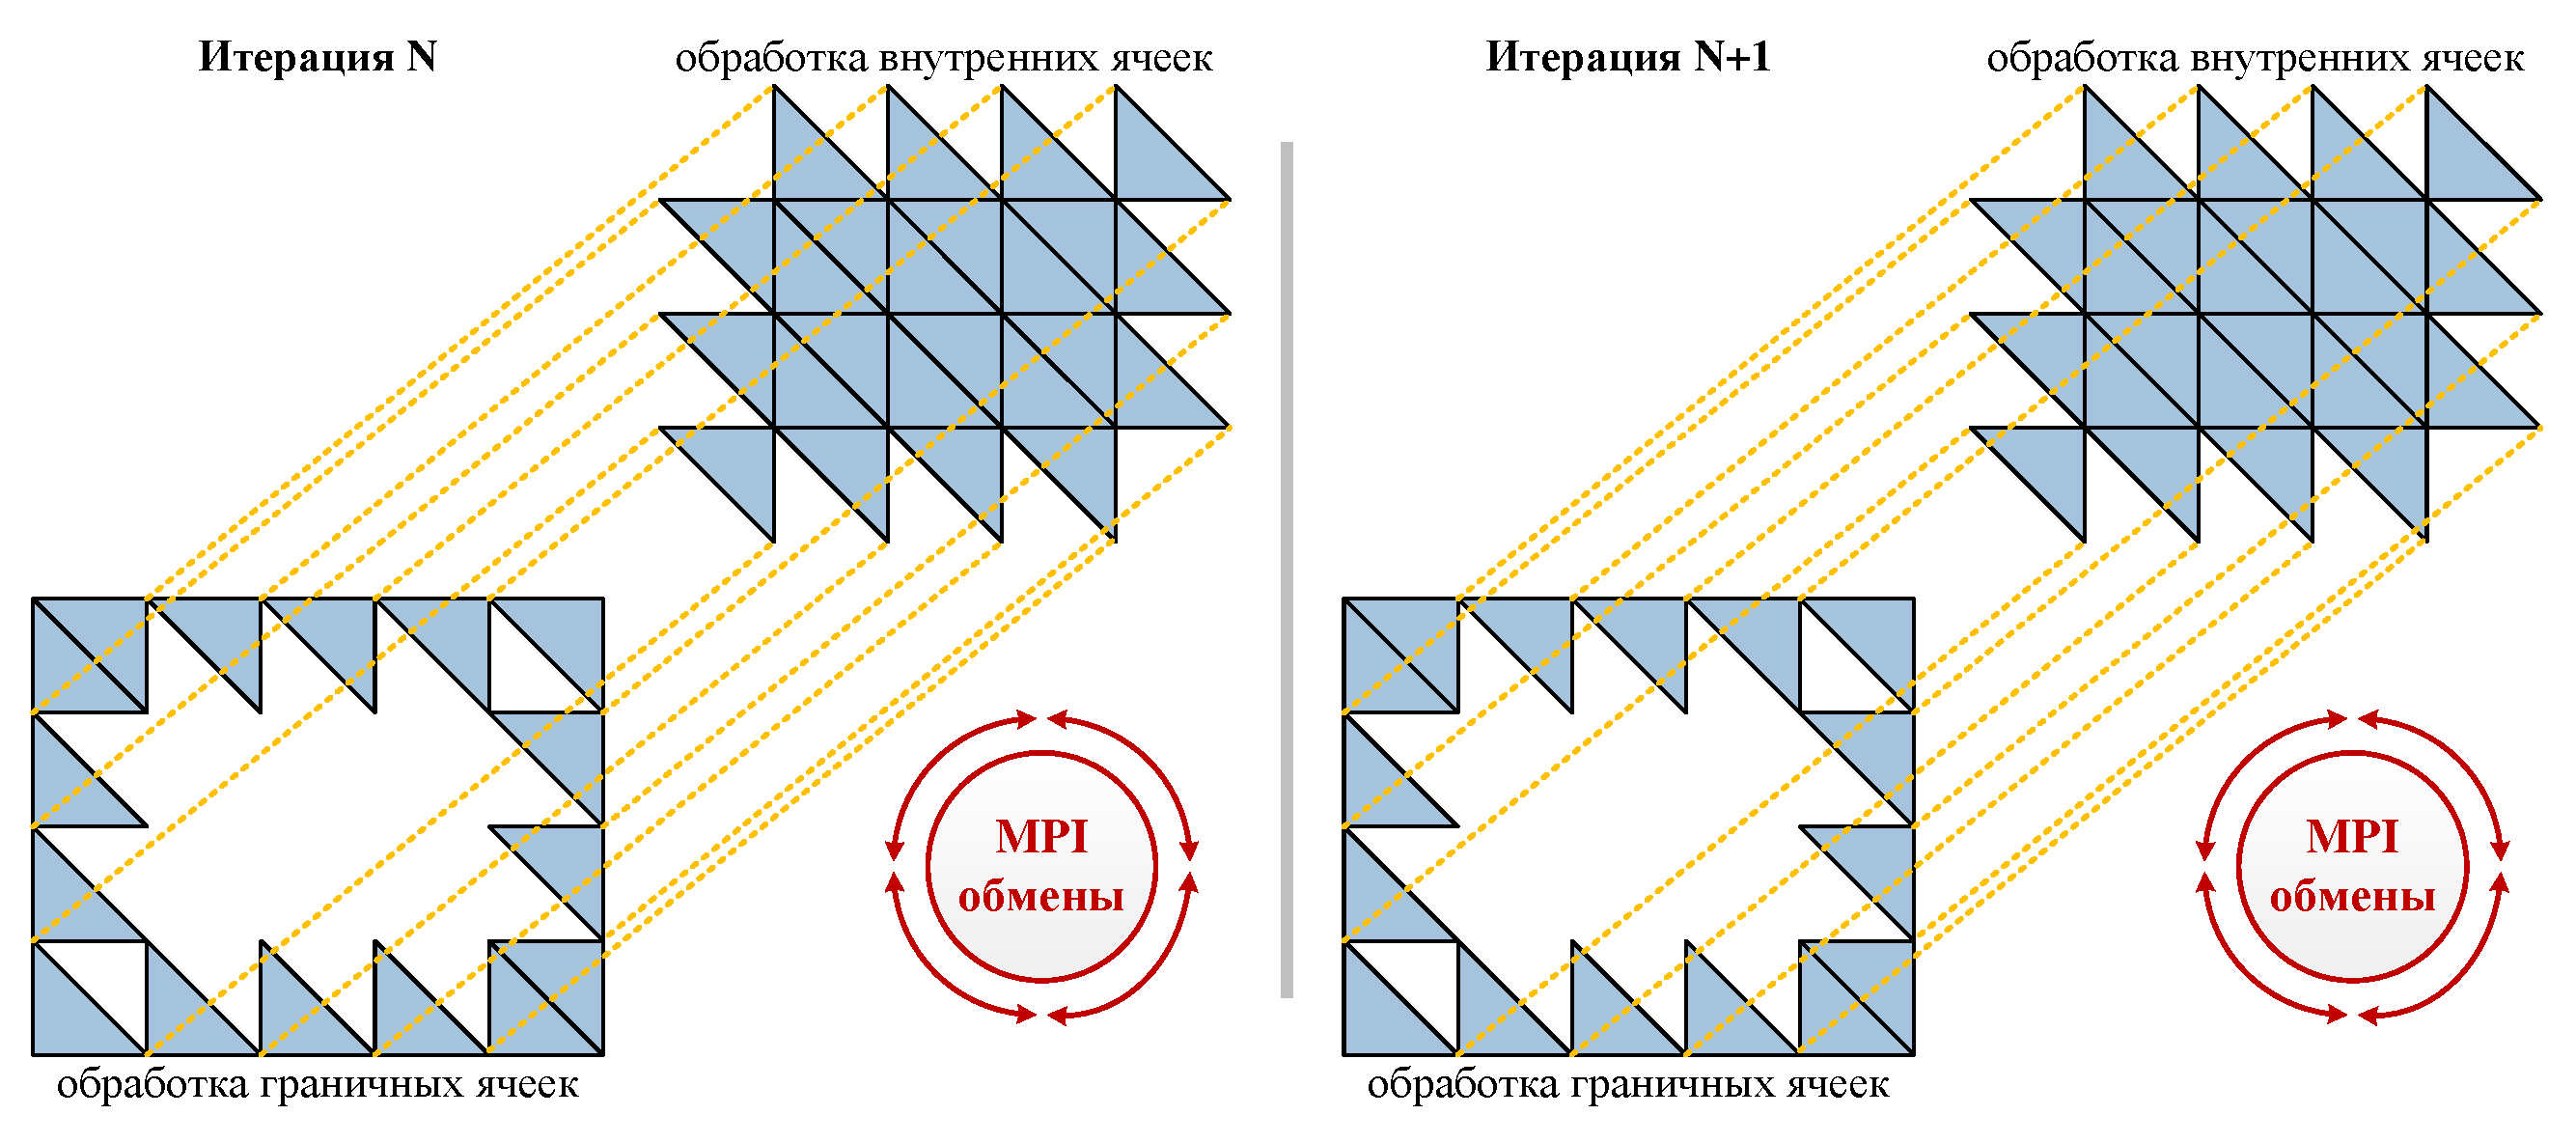
\includegraphics[width=0.8\textwidth]{./pics/text_2_decompsurf/mpi_border_inner.pdf}
\singlespacing
\captionstyle{center}\caption{Сокрытие издержек на информационные обмены за вычислениями.}
\label{fig:text_2_decompsurf_wing_border_inner}
\end{figure}

На этом этапе упомянем механизм частичного сокрытия издержек на обмены данными за основными вычислениями.
Все ячейки каждого домена можно разделить на внутренние\label{term:cell_block_inner2} и граничные\label{term:cell_block_border2} (аналогично внутренним и граничным ячейкам блока для блочно-структурированных сеток).
Ценность внутренних ячеек состоит в том, что они не участвуют в обменах данными с соседними доменами, поэтому обработку внутренних ячеек на следующей итерации расчетов можно начинать, не дожидаясь завершения обменов данными на ребрах, составляющих границу между доменами (см. рис.~\ref{fig:text_2_decompsurf_wing_border_inner}).
Понятно, что такой подход неприменим при использовании случайного распределения ячеек по доменам, так как в большинстве случаев множества внутренних ячеек доменов оказываются практически пустыми.

Рассмотрим семейство алгоритмов декомпозиции, в которых учитываются только индексы распределяемых ячеек и никак не учитываются другие их данные.
Под индексом в данном случае понимается номер ячейки в общем массиве ячеек расчетной сетки.
Уже по этому факту становится понятно, что такие алгоритмы не могут претендовать на высокое качество, так как их результат существенным образом зависит просто от порядка хранения данных расчетной сетки.
Самым простым из алгоритмов этого класса является алгоритм линейного распределения ячеек\label{term:alg_decomp_linear} по доменам.
Так как в каждый домен в среднем должно войти по $\frac{n}{k}$ ячеек (для простоты не будем обращать внимание на то, что это число может быть нецелым), то можно ячейки с номерами из диапазона $[0, \frac{n}{k} - 1]$ отнести к первому домену, ячейки с номерами $[\frac{n}{k}, \frac{2n}{k} - 1]$ ко второму домену и так далее.
При такой декомпозиции, конечно, можно добиться равномерного распределения ячеек по доменам, однако значения параметров $L$\label{term:decomp_maxbord2} и $I$\label{term:decomp_sumbord2} в общем случае предугадать невозможно.
Например, на рассматриваемой тестовой сетке видно, что деление на домены вдоль профиля крыла (как это показано на рис.~\ref{fig:text_2_decompsurf_4} сверху справа) порождает очень длинные границы между соседними доменами.
Было бы гораздо эффективнее производить деление сетки поперек профиля.

В общем случае ячейки с непрерывным диапазоном индексов не обязаны составлять не то что компактные домены с границами небольшой протяженности, а вообще могут порождать несвязные домены, с артефактами, выколотыми ячейками и так далее.
Применение таких алгоритмов оправдано только при обладании некоторой априорной информацией о структуре расчетной сетки (например, если известно, что сетка на самом деле является блочно-структурированной, в которой отдельные блоки соответствуют непрерывным диапазонам индексов ячеек).

Большой класс алгоритмов формируется из так называемых алгоритмов наращивания доменов\label{term:alg_decomp_rgrow}.
В основе этих алгоритмов лежит следующий принцип: вначале выбирается ячейка (или несколько ячеек), от которой далее производится наращивание домена путем последовательного добавления к ней соседних ячеек.
В рамках этого класса алгоритмов при последовательном создании доменов размера $\frac{n}{k}$ получим жадный алгоритм Фархата\label{term:alg_decomp_farhat}, результатом которого являются домены с очень протяженными границами \cite{Farhat1988Decomp}.
При использовании одновременного роста сразу нескольких доменов от случайных ячеек расчетной сетки получаем алгоритм пузырькового роста \cite{Preis1997Decomp}\label{term:alg_decomp_bubble}, который требуется запускать на расчетной сетке итерационно несколько раз для получения приемлемых характеристик качества разбиения.
При этом алгоритм пузырькового роста не гарантирует сбалансированного разбиения ячеек сетки по доменам (для достижения этого необходимо производить дополнительную коррекцию).
Также следует отметить инкрементальный алгоритм декомпозиции графов \cite{Yakobovsky2005Decomp}\label{term:alg_decomp_inc2}, особенностью которого является возможность освобождения части ячеек, уже распределенных по доменам, с последующим повторением роста доменов.

Мы рассматриваем простой алгоритм наращивания доменов, в котором все домены наращиваются одновременно, начиная с некоторых случайно выбранных ячеек сетки.
При этом поддерживается связность доменов -- если в какой-то момент домену больше некуда расти, то он прекращает свое наращивание и больше не расширяется.
Таким образом, возможно генерация крайне неравномерных по количеству ячеек доменов. Пример результата применения описанного алгоритма приведен на рис.~\ref{fig:text_2_decompsurf_4} снизу слева.

Кроме приведенных алгоритмов существует еще большое количество подходов к декомпозиции расчетных сеток, среди них алгоритмы, основанные на методе спектральной бисекции \cite{Urschel2014Decomp}, диффузионные и генетические алгоритмы \cite{Zhao2019Decomp}, иерархические алгоритмы \cite{Kapyris1998Decomp} и многие другие.
Наиболее полный обзор различных алгоритмов декомпозиции расчетных сеток можно найти в \cite{Golovchenko2020Decomp} и \cite{Zheleznyakova2017Decomp}.

\subsubsection{Алгоритм декомпозиции с помощью иерархического \\ дробления}\label{sec:text_2_decompsurf_hierarchical}

\label{term:alg_decomp_inc}В работе \cite{Golovchenko2020Decomp} описан параллельный алгоритм геометрической декомпозиции сеточных данных.
Во время работы этого алгоритма происходит последовательное деление текущего домена пополам с помощью сечения плоскостью.
На рис.~\ref{fig:text_2_decompsurf_hierarchical} продемонстрирована схема, по которой изначальный головной домен h делится на пару доменов hl (left), hr (right), каждый из которых делится далее пополам и так далее на любое количество доменов, равное степени двойки.

\begin{figure}[ht]
\centering
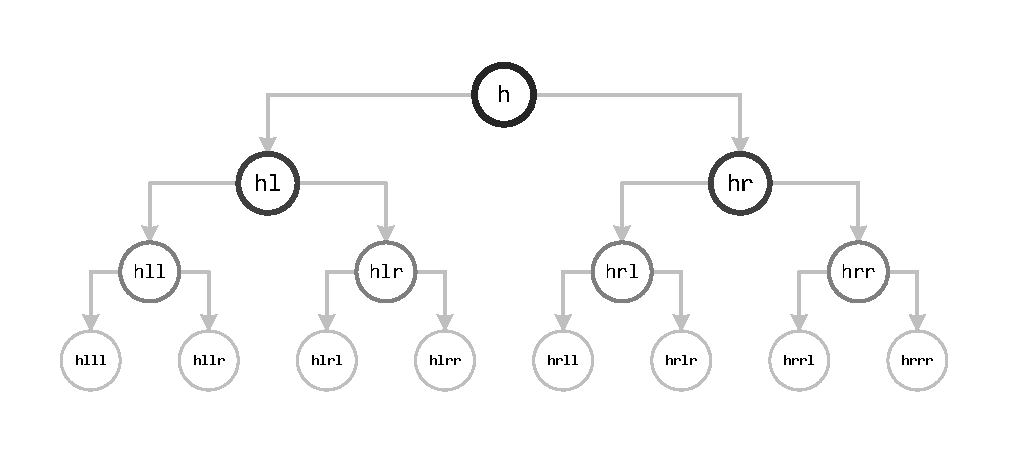
\includegraphics[width=0.6\textwidth]{./pics/text_2_decompsurf/hierarchical.pdf}
\singlespacing
\captionstyle{center}\caption{Иллюстрация иерархического трехуровневого разделения головного домена.}
\label{fig:text_2_decompsurf_hierarchical}
\end{figure}

Этот алгоритм предлагается расширить, введя в него произвольные критерии разбиения текущего домена на пару более мелких доменов.
Вначале рассмотрим схему простого деления домена пополам с использованием произвольного признака, по которому производится деление (см. рис.~\ref{fig:text_2_decompsurf_split}).

\begin{figure}[ht]
\centering
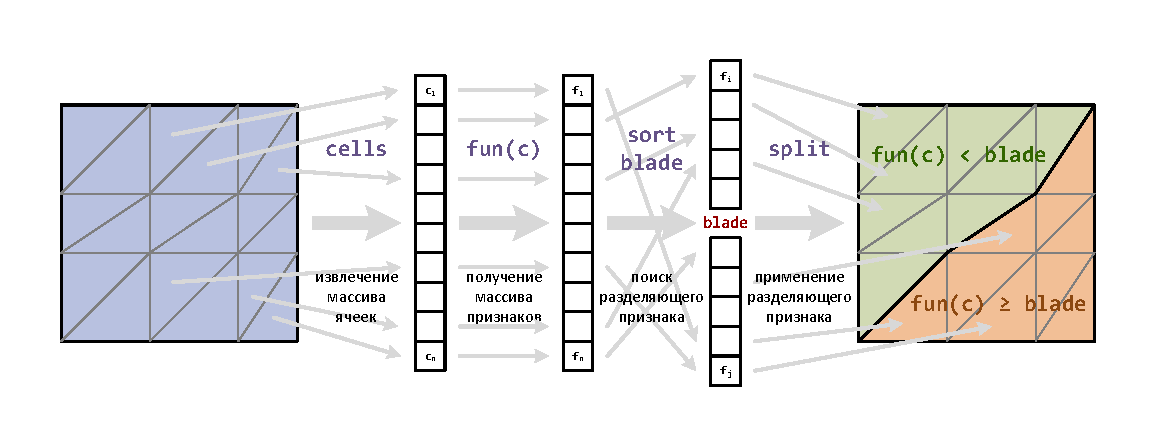
\includegraphics[width=0.9\textwidth]{./pics/text_2_decompsurf/split.pdf}
\singlespacing
\captionstyle{center}\caption{Схема выполнения разделения домена пополам по заданному признаку fun.}
\label{fig:text_2_decompsurf_split}
\end{figure}

Пусть задан массив ячеек домена $C$ и произвольная функция извлечения признака из ячейки $fun$.
Первым шагом является вычисление массива признаков для всех ячеек.
После этого половина массива с меньшими значениями признака формирует один дочерний домен, а вторая половина с большими значениями признакак формирует второй дочерний домен.

После разделения домена на два более мелких домена можно вычислить параметр, отражающий эффективность разбиения.
В качестве такого параметра предлагается использовать длину границы между двумя образованными новыми доменами.
Таким образом, критерий разбиения зависит от функции вычисления признака $fun$.
В свою очередь это означает, что при выполнении разбиения не обязательно ограничиваться одной функцией вычисления признака, вместо этого можно подать список функций, для каждой функции вычислитель показатель качества разбиения и в результате остановиться на той функции вычисления признака, которая в конечном итоге приводит к наиболее эффективному разбиению.
Если в качестве функций вычисления признака ячейки использовать просто извлечение трех координат центров ячеек, то мы получим в чистом виде алгоритм геометрической декомпозиции сетки с выбором для дробления наиболее протяженного размера по одной из координат.
Результат применения этого алгоритма показан на рис.~\ref{fig:text_2_decompsurf_4} снизу справа.

Варьируя набор функций вычисления признаков, по которым можно выполнять разбиение домена, возможно выполнять геометрическую декомпозицию вдоль направления любой кривой, для которой вычисляется проекция ячейки.
Декомпозиция с помощью данного метода не ограничивается только геометрическими признаками.
Функции вычисления признаков могут использоваться для анализа физических данных ячеек, например, для локализации и выделении в отдельные домены областей с повышенным давлением.

\subsubsection{Результаты экспериментов по декомпозиции расчетных \\ сеток на профиле крыла}

\begin{figure}[H]
\centering
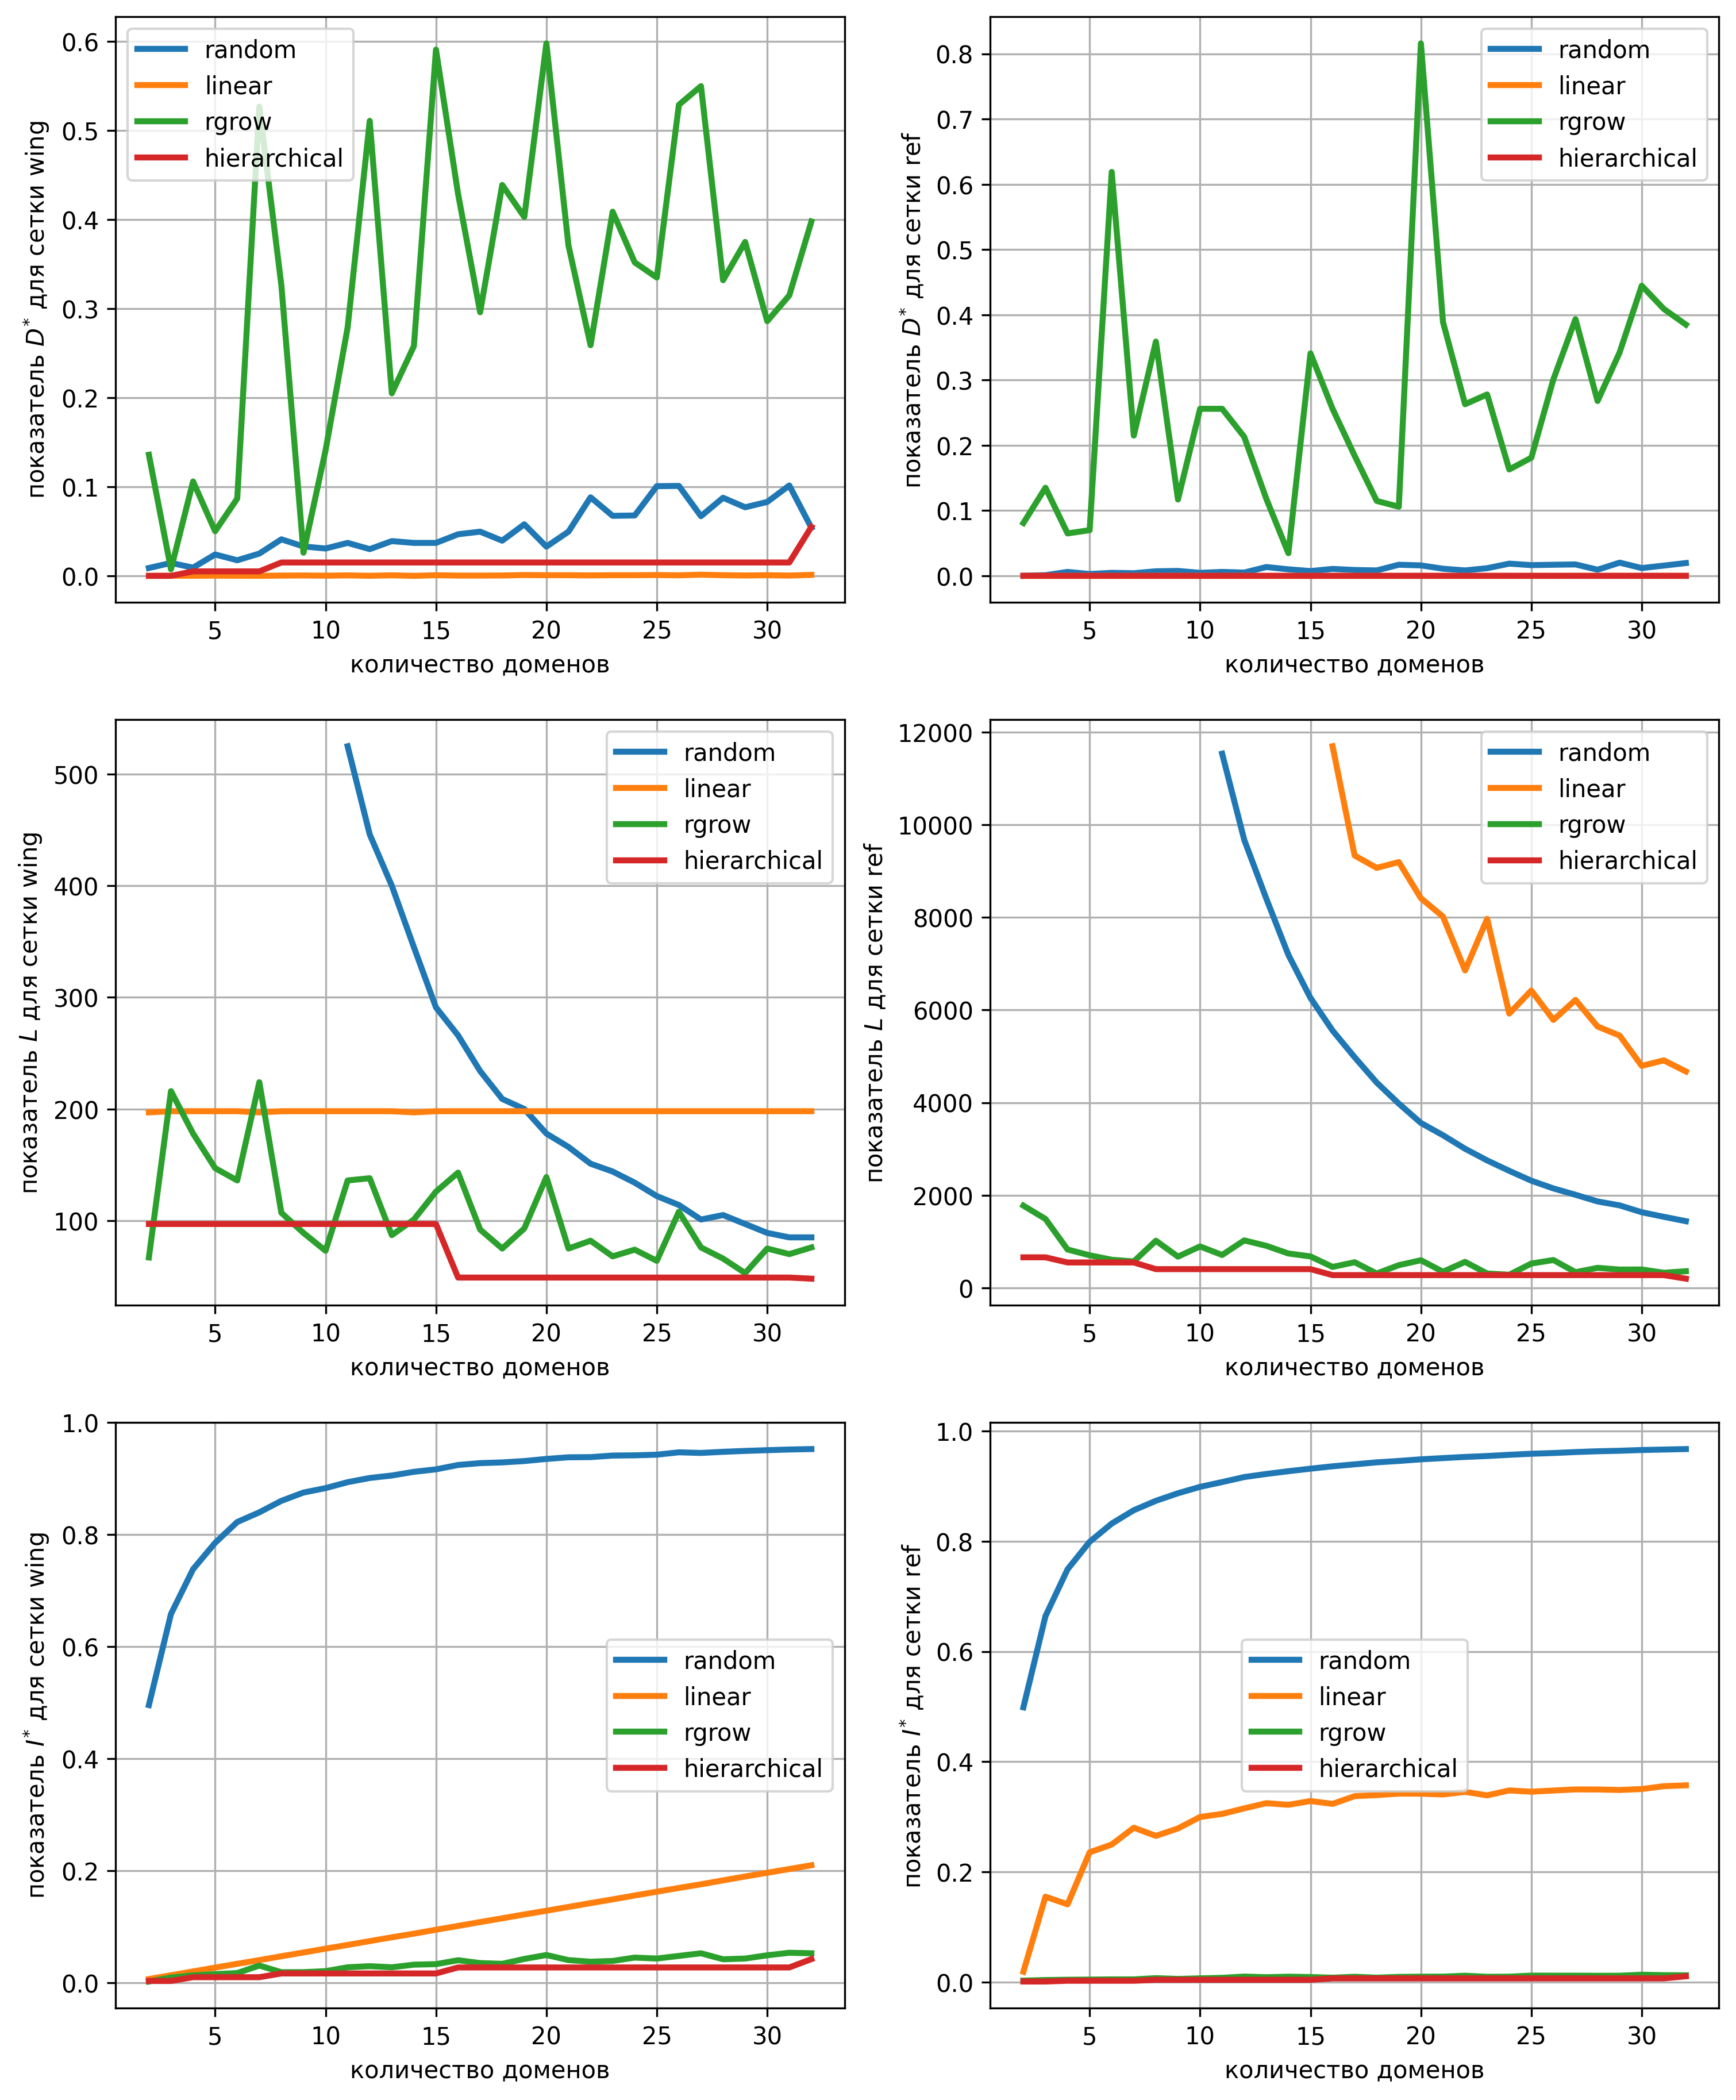
\includegraphics[width=1.0\textwidth]{./pics/text_2_decompsurf/qual.png}
\singlespacing
\captionstyle{center}\caption{Графики показателей $D^{*}$, $L$, $I^{*}$ для сеток wing и ref.}
\label{fig:text_2_decompsurf_qual}
\end{figure}

На рис.~\ref{fig:text_2_decompsurf_qual} представлены графики параметров $D^{*}$, $L$, $I^{*}$, вычисленные во время применения различных алгоритмов декомпозиции поверхностной расчетной сетки на разное количество доменов от 2 до 32.

Для эксперимента использовались две сетки.
Первая сетка -- wing, представленная на рис.~\ref{fig:text_2_decompsurf_wing_grid}.
Вторая сетка -- ref -- более приближена к реальной геометрии летательного аппарата и содержит порядка $n = 4 \cdot 10^5$ ячеек.
На графиках введены следующие краткие названия алгоритмов: random -- случайное распределение ячеек по доменам\label{term:alg_decomp_random2}, linear -- линейное разделение ячеек между доменами по индексу\label{term:alg_decomp_linear2}, rgrow -- алгоритм наращивания доменов от случайных ячеек\label{term:alg_decomp_rgrow2}, hierarchical -- иерархическое дробление доменов\label{term:alg_decomp_hierarch2} пополам по одной из трех координат (в качестве функций вычисления признаков ячеек брались просто функции извлечения каждой из трех координат центра ячейки).

При этом отметим, что при использовании алгоритма rgrow умышленно использовалась только одна итерации наращивания, для демонстрации того, насколько неравномерным может быть распределение размеров доменов при случайном выборе инициирующих ячеек (из рисунков видно, что значение параметра $D^{*}$\label{term:decomp_neravn4} достигает значениий 0,6 и 0,8 для сеток wing и ref соответственно).

Из приведенных графиков можно сделать выводы, что из представленных алгоритмов иерархическое деление доменов с выбором оптимального критерия деления из списка функций вычисления признаков ячеек является наиболее приемлемым по параметрам $D^{*}$, $L$,\label{term:decomp_maxbord3} $I^{*}$,\label{term:decomp_sumbord3} то есть с помощью этого алгоритма генерируется достаточно равномерное распределение ячеек по доменам при низкой общей доле междоменных ребер и малой протяженности границ между доменами.

% Генетический алгоритм декомпозиции расчетной сетки.
\subsubsection{Генетический алгоритм декомпозиции \\ неструктурированной расчетной сетки}\label{sec:text_2_genetic}

\label{term:alg_decomp_gen}Генетические алгоритмы представляют собой природоподобные эвристические алгоритмы, с помощью которых можно искать решения оптимизационных задач с большим количеством параметров \cite{Chahar2021Gen,Wirayanti2025Gen}.
В процессе применения генетического алгоритма моделируется процесс создания, выживания и размножения популяции потенциально возможных решений поставленной проблемы в условиях сложно устроенной окружающей среды.
Применимость генетических алгоритмов базируется на принципе выживания сильнейших особей в популяции \cite{Naaman2025Gen}.
Работа генетического алгоритма начинается с создания стартовой популяции потенциальных решений проблемы, каждое решение представлено отдельной особью, а каждая особь определяется набором характеризующих ее генов (генотипом)\label{term:genotype}.
Для особи должна быть определена функция пригодности, которая является индикатором качества особи для решения поставленной задачи (вместо функции пригодности можно использовать штрафную функцию\label{term:penalty_function}, которая наоборот является показателем непригодности). 

Генетический алгоритм является итерационным.
На каждой итерации по определенным законам на основе текущей популяции создается следующая популяция\label{term:population}, которая по ожиданиям в среднем должна быть более приспособлена к условиям окружающей среды (то есть лучше удовлетворять решению поставленной задачи).
Процесс получения новых популяций продолжается до тех пор, пока не будет достигнуто некоторое условие (либо получено решение требуемого качества, либо дальнейшее улучшение не наблюдается) \cite{Charilogis2024Gen}.
Генетические алгоритмы широко применяются во многих областях, для решения задач с большим количеством параметров и ограничений.
Конечно, применение генетических алгоритмов не подразумевает отыскание оптимального решения, однако с их использованием можно быстро найти решение, которое является достаточно качественным в текущих условиях.
Генетические алгоритмы применимы для решения задач планирования \cite{Dawei2025Gen} и эффективного использования ресурсов \cite{Fang2025Gen,Mahmood2024Gen}.
Они используются для анализа данных, поиска тенденций и предсказаний, где не могут быть получены точные решения \cite{Kangra2024Gen,Sangeetha2025Gen}.
Одна из областей активного применения генетических алгоритмов – задачи комбинаторной оптимизации \cite{Hamdan2023Comb,Odeyemi2025Comb}.
При решении задач комбинаторной оптимизации точное решение зачастую не может быть получено из-за большого количества параметров и отсутствия полиномиального алгоритма для решения поставленной проблемы.
Генетические алгоритмы позволяют находить приемлемые решения для таких классических задач, как задача коммивояжера \cite{Kralev2024Gen}, задача нахождения оптимального пути \cite{Bogdanov2023Gen}, раскраска графа \cite{Malhotra2024Graph}, декомпозиция графа \cite{Chaouche2023Graph,Li2020Graph}.

При использовании генетических алгоритмов важно различать понятие генотипа и особи.
Генотип – это набор генов, некий код, который кодирует механизм создание особи.
Особь – сформированный на основе генотипа индивид, который обладает определенными свойствами и характеристиками, и для которого может быть вычислена функция пригодности или штрафная функция.
Зачастую при использовании генетических алгоритмов различие между генотипом и особью стирается, и вместо генотипа используется просто явное представление особи.
Так в работе \cite{Chaouche2023Graph} при декомпозиции графа в генотипе кодируется каждое ребро рассматриваемого графа, а в работе \cite{Li2020Graph} генотип представляет собой точное соотнесение каждой вершины графа и результирующего домена.
Использование генотипа в роли особи в генетических алгоритмах приводит к существенному замедлению сходимости, что снижает ценность использования этих алгоритмов.
К тому же применение механизмов скрещивания и мутаций к особям вместо генотипов также вызывает сомнение с точки зрения корректности таких операций.
В этом разделе предлагается подход, в котором в качестве генотипа используется максимально короткий код, по которому может быть быстро построена особь.

\subsubsection{Описание алгоритма}

Рассмотрим алгоритм декомпозиции дуального графа\label{term:dual_graph2} произвольной расчетной сетки на $k$ доменов.
Количество вершин в графе равно $n$.
При этом рассматриваемый дуальный граф задан структурами \texttt{inc} и \texttt{es}.
В структуре \texttt{inc} хранятся соседи каждой вершины графа: \texttt{inc[i]} -- вектор номеров всех вершин, смежных $i$-й вершине.
Структура \texttt{es} -- множество ребер графа.

В качестве особи будем рассматривать вектор \texttt{domains} длины $n$, в котором \texttt{domains[i]} -- номер домена\label{term:domain4}, к которому отнесена $i$-ая вершина графа.
В качестве функции качества особи будем использовать функцию $Q = \delta D + \lambda L$ (чем ниже значение данной функции, тем выше качество особи) с весами $\delta = 10$ и $\lambda = 1$.
Исходя из этого, функцию $Q$ можно называть штрафной функцией особи.
Под популяцией будем понимать набор отдельных особей.

Ключевым элементом генетического алгоритма является понятие генотипа и процесс формирования особи на основе генотипа.
В качестве генотипа будем использовать вектор \texttt{genotype} длины $k$, задающий $k$ номеров вершин дуального графа, которые будем называть опорными вершинами\label{term:opor_point}.
При инициализации каждую опорную вершину \texttt{genotype[i]} будем принудительно относить к $i$-му домену.
При построении особи на основе генотипа будем распределять вершины между доменами с помощью простого алгоритма, схожего с алгоритмом пузырькового роста, начиная с опорных вершин и обходя граф в ширину.
Программный код процедуры распределения вершин между доменами можно видеть на листинге~\ref{lst:text_2_gen_alg}.

\begin{singlespace}
\begin{lstlisting}[caption={Простая декомпозиция, используемая в генетическом алгоритме.},label={lst:text_2_gen_alg}]
deque<size_t> q;

for (auto i { 0 }; i < k; ++i)
{
    domains[genotype[i]] = i;
    q.push_back(genotype[i]);
}

while (!q.empty())
{
    auto node { q.front() };
    auto domain { domains[node] };
    q.pop_front();

    for (auto ngh : inc[node])
    {
        if (domains[ngh] == -1)
        {
            domains[ngh] = domain;
            q.push_back(ngh);
        }
    }
}
\end{lstlisting}
\end{singlespace}

Приведенный на листинге~\ref{lst:text_2_gen_alg} алгоритм декомпозиции по опорным вершинам не является сколь угодно оптимальным (и даже намеренно взят наиболее простым) и создает несбалансированные разбиения, зато он является быстрым, что позволяет создавать большое количество особей за короткое время.

На основе выбранного простого способа построения особи будем моделировать процесс эволюции следующим образом.
Пусть мы имеем текущую популяцию, в которой для каждой особи известна характеристика ее качества (эта характеристика вычисляется при построении особи и не меняется на протяжении всей ее жизни).
На первой фазе будем удалять некоторое количество наихудших особей из популяции.
Из оставшейся популяции случайно сформированные пары особей на основе операции скрещивания (кроссовера)\label{term:crossover} будут производить потомство и добавлять в популяцию для восстановления ее исходного размера.
Операция скрещивания устроена предельно просто: для каждого номера $i$ от $1$ до $k$ в качестве $i$-го гена случайным образом выбирается $i$-й ген одного из родителей.
После выполнения скрещивания в новой особи с заданной вероятностью применяется мутация (см. рис.~\ref{fig:text_2_genetic_cross_mut})\label{term:mutation}.

\begin{figure}[ht]
\centering
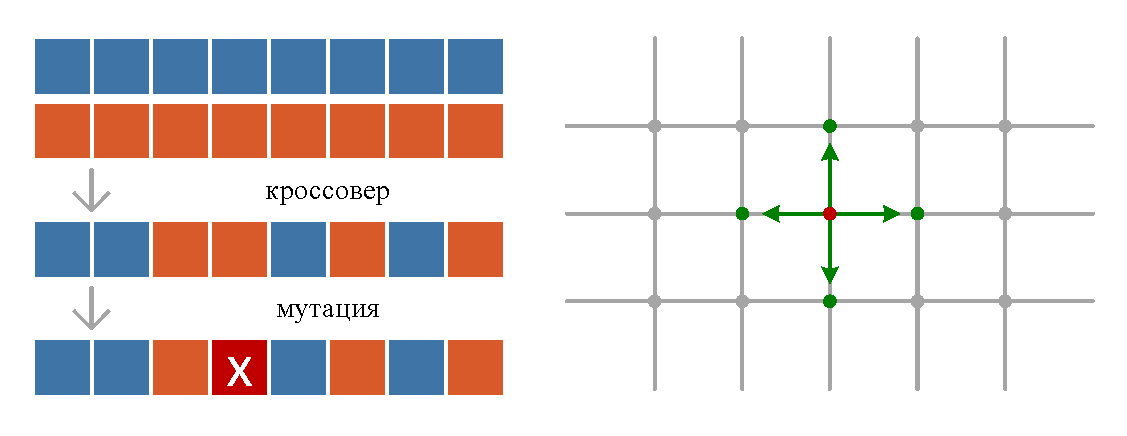
\includegraphics[width=0.7\textwidth]{./pics/text_2_genetic/cross-mut.pdf}
\singlespacing
\captionstyle{center}\caption{Схема кроссовера и мутации новой особи.}
\label{fig:text_2_genetic_cross_mut}
\end{figure}

Так как ген представляет собой номер опорной вершины дуального графа, то в качестве мутации выбрана операция замены случайной опорной вершины на выбранную случайным образом смежную с ней вершину (см. рис.~\ref{fig:text_2_genetic_cross_mut}, справа).

Описанный генетический алгоритм поиска эффективной декомпозиции характеризуется следующими глобальными параметрами. Количество эпох (\texttt{epochs\_count}) -- количество последовательных применяемых глобальных операций по вымиранию части популяции и ее восстановлению.
Размер популяции особей (\texttt{population\_size}) -- количество особей в популяции.
Доля вымирания (\texttt{extinction\_ratio}) – доля наименее эффективных особей, вымирающих на каждой эпохе.
Вероятность мутации (\texttt{mutation\_propability}) -- вероятность мутации в новой особи.

\subsubsection{Эксперимент по применению генетического алгоритма}

Будем применять описанный выше генетический алгоритм для решения задачи декомпозиции двумерной прямоугольной расчетной сетки размером $100 \times 100$ ячеек.
Такой вид сетки выбран для удобства визуализации результатов, сам алгоритм применим для расчетных сеток произвольного вида, так как на вход он принимает только информацию о структуре дуального графа.

Количество параметра \texttt{epochs\_count} выбрано равным 500.
Алгоритм прекращает работу либо после обработки последней эпохи, либо после того, как все особи в популяции сравняются по характеристике эффективности.

Размер популяции \texttt{population\_size} выбран равным 50.
При выборе размера популяции необходимо придерживаться баланса.
При слишком большом значении этого параметра время работы алгоритма существенно возрастает, а при слишком маленьком значении ограничивается разнообразие особей в популяции, что приводит к ранней остановке алгоритма в локальном минимуме, в котором все особи обладают одинаковым достаточно плохим показателем эффективности.

Доля вымирания \texttt{extinction\_ratio} принята равной 0,2.
При выборе доли вымирания не стоит использовать слишком высокие значения, так как это приводит к излишне интенсивному отсеву особей.
Это может привести к преждевременной отбраковке средних по эффективности особей, способных дать более эффективное потомство.

Вероятность возникновения мутации \texttt{mutation\_probability} принята равной 0,2.
Ввиду того, что мутация представляет собой смещение опорной вершины по ребру к одному из своих соседей (что является достаточно незначительным изменением), то такое частое возникновение мутаций оправдано.

\begin{figure}[ht]
\centering
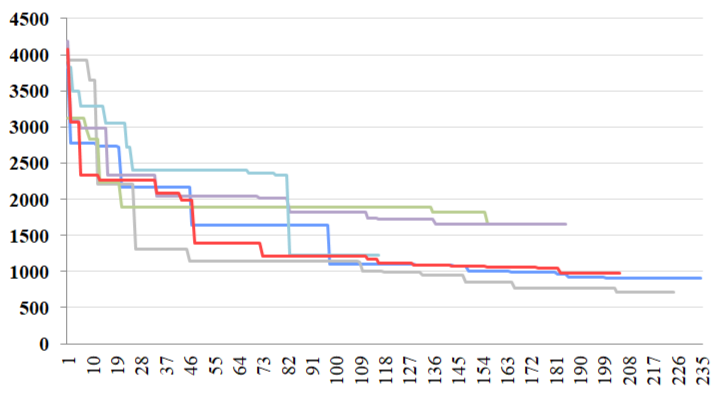
\includegraphics[width=0.8\textwidth]{./pics/text_2_genetic/chart1.png}
\singlespacing
\captionstyle{center}\caption{Характерные графики штрафной функции лучшей особи в популяции в зависимости от номера эпохи.}
\label{fig:text_2_genetic_chart1}
\end{figure}

Типичные графики значения штрафной функции лучшей особи в популяции от номера эпохи приведены на рис.~\ref{fig:text_2_genetic_chart1}.
Эксперименты показали, что при выбранном наборе макропараметров алгоритма примерно в первые 100 эпох наблюдается существенное улучшение лучшей особи в популяции, затем медленное улучшение наблюдается еще около 150 эпох, после чего работа алгоритма останавливается в локальном минимуме при заполнении всей популяции копиями лучшей особи.
При этом значение штрафной функции лучшей особи за время работы алгоритма падает примерно на 50-75\%, если считать от значения лучшей особи стартовой популяции.
Для повышения качества работы алгоритма можно включить механизм предотвращения его ранней остановки.
Для этого при возникновении копий лучшей особи можно применять к ней так называемые макромутации, что соответствует принудительному выталкиванию особи из локального минимума штрафной функции \cite{Baranov2025Gen}.

\begin{figure}[ht]
\centering
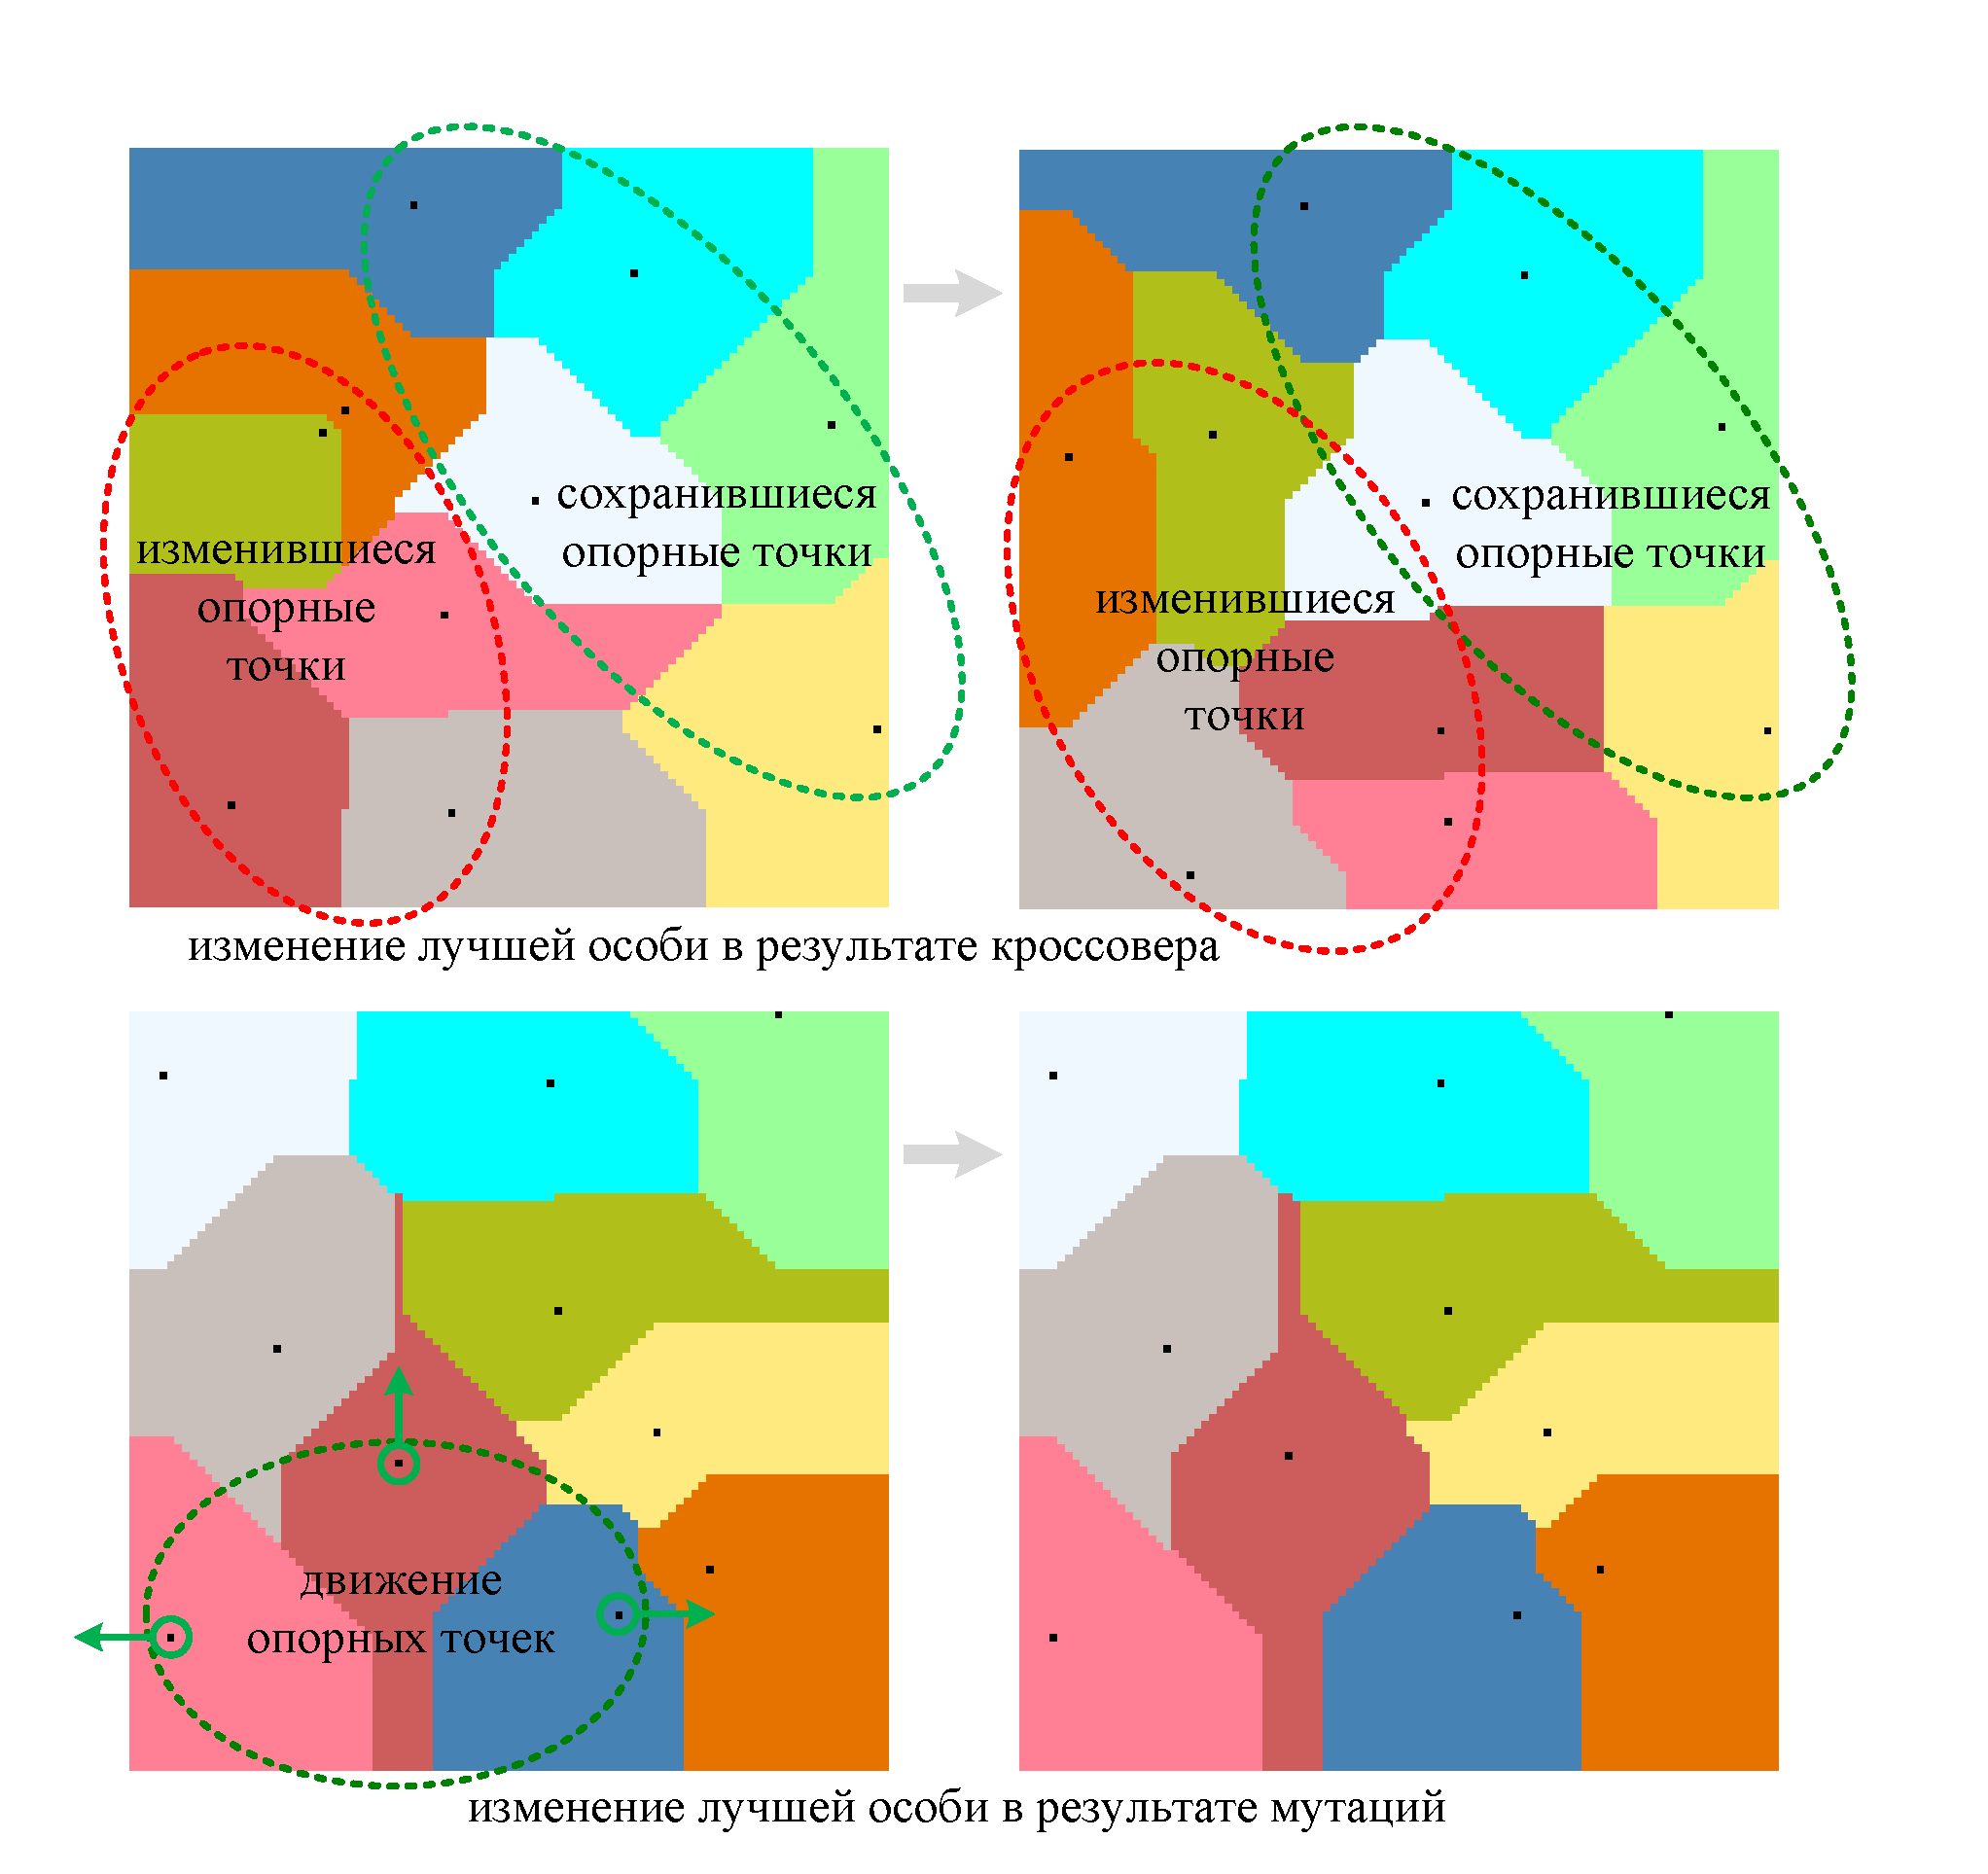
\includegraphics[width=0.8\textwidth]{./pics/text_2_genetic/changes.pdf}
\singlespacing
\captionstyle{center}\caption{Замещение части генотипа\label{term:genotype2} в процессе скрещивания (сверху), и мутация опорных вершин\label{term:opor_point2} (снизу).}
\label{fig:text_2_genetic_changes}
\end{figure}

На рис.~\ref{fig:text_2_genetic_changes} приведены характерные варианты изменения лучшей особи при переходе от текущей популяции к популяции следующей эпохи.
Сверху на рисунке проиллюстрирована ситуация, когда часть опорных вершин лучшей особи сохранилась, а другая часть была заменена на опорные вершины второго родителя, что в целом привело к снижению значения штрафной функции.
Снизу на рисунке проиллюстрировано влияние последовательности мутаций на лучшую особь.
Так, даже незаметное на рисунке смещение опорных вершин привело к визуально различимому изменению геометрии образованных этими опорными вершинами доменов.

Следует отметить, что хоть реализация генетического алгоритма и подразумевает постоянное улучшение эволюционирующей популяции, это никак не гарантируется.
Более того, при скрещивании двух особей нет гарантии, что их потомство будет более приспособленным к поставленной задаче.
Также отсутствует гарантия, что применяемые мутации всегда приводят к более качественному решению.
Поэтому возникает вопрос -- не является ли сам факт появления удачных особей случайным событием, и не было бы более эффективным просто сгенерировать большое количество случайных особей, после чего выбрать из них лучшего представителя.
Для проверки этого предположения были проведены следующие эксперименты.
Пусть у нас имеется одиночный запуск генетического алгоритма с макропараметрами \texttt{population\_size} и \texttt{extinction\_ratio}.
Если в процессе работы алгоритма до его завершения прошло \texttt{ecount} эпох (не считая стартовой), то всего было создано \texttt{icount} = \texttt{population\_size} × (1 + \texttt{ecount} × \texttt{extinction\_ratio}) особей.
Поэтому после завершения каждого запуска генетического алгоритма его результат сравнивался со значением лучшей особи из случайной популяции размера \texttt{icount}.
Результаты такого сравнения приведены на рис.~\ref{fig:text_2_genetic_chart2}.
Красным цветом отмечен график качества лучшей особи в начале работы алгоритма, зеленым -- в конце.
Черным цветом отмечено значение лучшей особи случайной популяции размера \texttt{icount}.
Также на графиках отмечены линии средних значений для серии запусков генетического алгоритма.
Результаты расчетов показали, что лучшая особь популяции генетического алгоритма опережает лучшую особь случайной популяции примерно в 1,5 раза.

\begin{figure}[ht]
\centering
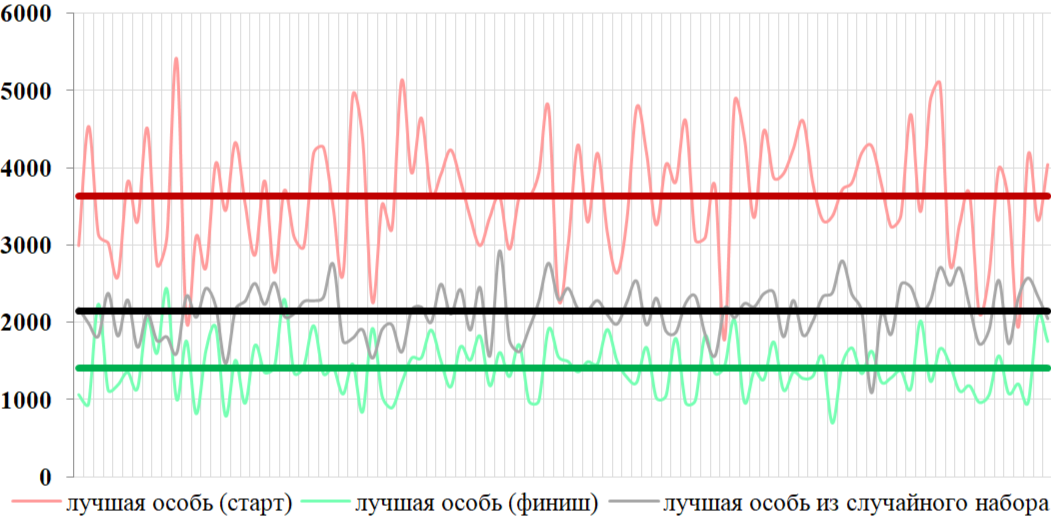
\includegraphics[width=0.8\textwidth]{./pics/text_2_genetic/chart2.png}
\singlespacing
\captionstyle{center}\caption{Сравнение лучшей особи в популяции генетического алгоритма с лучшей особью случайной популяции.}
\label{fig:text_2_genetic_chart2}
\end{figure}

Разработанный генетический алгоритм применим к расчетным сеткам произвольного вида, с его помощью можно быстро получать качественное решение декомпозиции, произвольным образом задавая требуемую штрафную функции решения.
Алгоритм допускает параллельное исполнение, хорошо масштабируется для работы с расчетными сетками большего размера.
Алгоритм может быть расширен с помощью других процедур генерации особи из генотипа.
В совокупности с генетическим алгоритмом декомпозиции для поверхностных расчетных сеток\label{term:unstruct_surf_calc_mesh5} может быть применен алгоритм сглаживания границ между доменами\label{term:alg_smooth_domains_border2} из раздела~\ref{sec:text_2_smooth}, с помощью которого можно не только уменьшить длину границ между доменами, но и скорректировать баланс ячеек между доменами для улучения показателя качества декомпозиции $D$.\label{term:decomp_neravn7}

% Сглаживание границ доменов.
\subsubsection{Сглаживание границ между доменами \\ поверхностной расчетной сетки}\label{sec:text_2_smooth}

При использовании декомпозиции расчетной сетки основным показателем качества декомпозиции является параметр $D$\label{term:decomp_neravn5}, так как он отражает равномерность распределения ячеек по разным вычислительным процессам.
Однако если игнорировать остальные показатели, то в процессе декомпозиции могут появляться протяженные <<пилообразные>> границы между доменами\label{term:domain3}, которые приводят к возрастанию параметров качества декомпозиции $L$\label{term:decomp_maxbord4} и $I$\label{term:decomp_sumbord4}, что негативно сказывается на производительности.
Пример возникновения таких пилообразных границ можно увидеть на рис.~\ref{fig:text_2_decompsurf_4} снизу справа, на рис.~\ref{fig:text_2_smooth_bad_border} фрагмент сетки с пилообразными границами между доменами приведен более крупно.

\begin{figure}[ht]
\centering
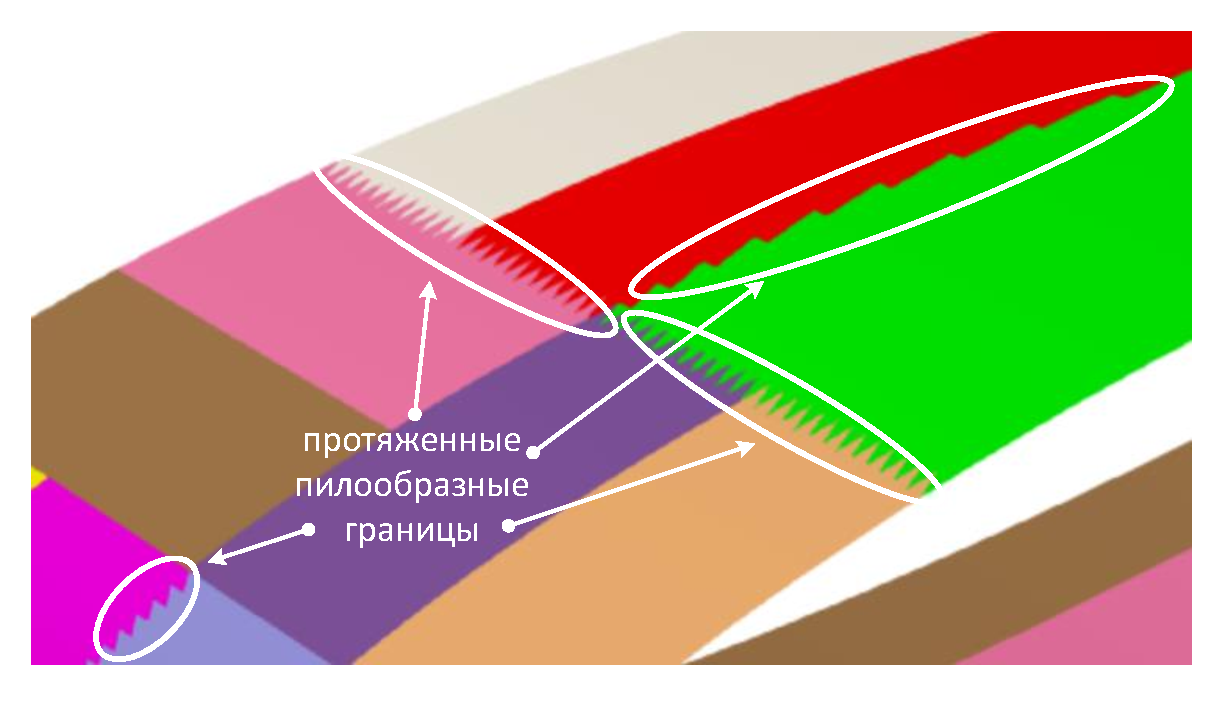
\includegraphics[width=0.6\textwidth]{./pics/text_2_smooth/bad-border.pdf}
\singlespacing
\captionstyle{center}\caption{Возникновение протяженных пилообразных границ между доменами.}
\label{fig:text_2_smooth_bad_border}
\end{figure}

Конечно такие границы необходимо отдельно обрабатывать с целью сокращения их длины.
При использовании алгоритмов декомпозиции, основанных на наращивании доменов\label{term:alg_decomp_rgrow3} путем обхода графа в ширину, образуются более сглаженные границы, однако из-за этого деградирует параметр качества декомпозиции $D$.
Возникновение протяженных пилообразных границ между доменами особенно характерно для неструктурированных поверхностных сеток, на которых зачастую встречаются ячейки с очень острыми углами.
Будем рассматривать алгоритм сглаживания границ между доменами, на который дополнительно накладывается требование сохранения параметра $D$ \cite{Bagrov2021Smooth}.

\subsubsection{Алгоритм сглаживания границ между доменами}

Алгоритм сглаживания\label{term:alg_smooth_domains_border} носит локальный характер, он применяется последовательно к каждой паре доменов и направлен на уменьшение длины границы между ними с сохранением баланса количества ячеек в этих доменах.
Граница между двумя доменами может быть представлена в виде набора простых циклов и простых цепей.
При этом простой цикл может быть обработан таким же образом, как и простая цепь, с учетом совпадения первого и последнего узла этой цепи (для такого виртуального размыкания простого цикла может быть выбран произвольный узел этого цикла).
В процессе применения алгоритма сглаживания может быть выполнено виртуальное размыкание всех простых циклов, после чего все образовавшиеся цепи рассматриваются последовательно.
Без ограничения общности можно считать, что мы работаем с одной простой цепью (полученной с помощью записи всех отдельных простых цепей подряд), представляющей границу между парами доменов.

Вначале одним линейным проходом по цепи выполняется поиск всех пригодных для сглаживания границы шаблонов\label{term:smooth_template}, представленных на рис.~\ref{fig:text_2_smooth_smooth_border}.

\begin{figure}[ht]
\centering
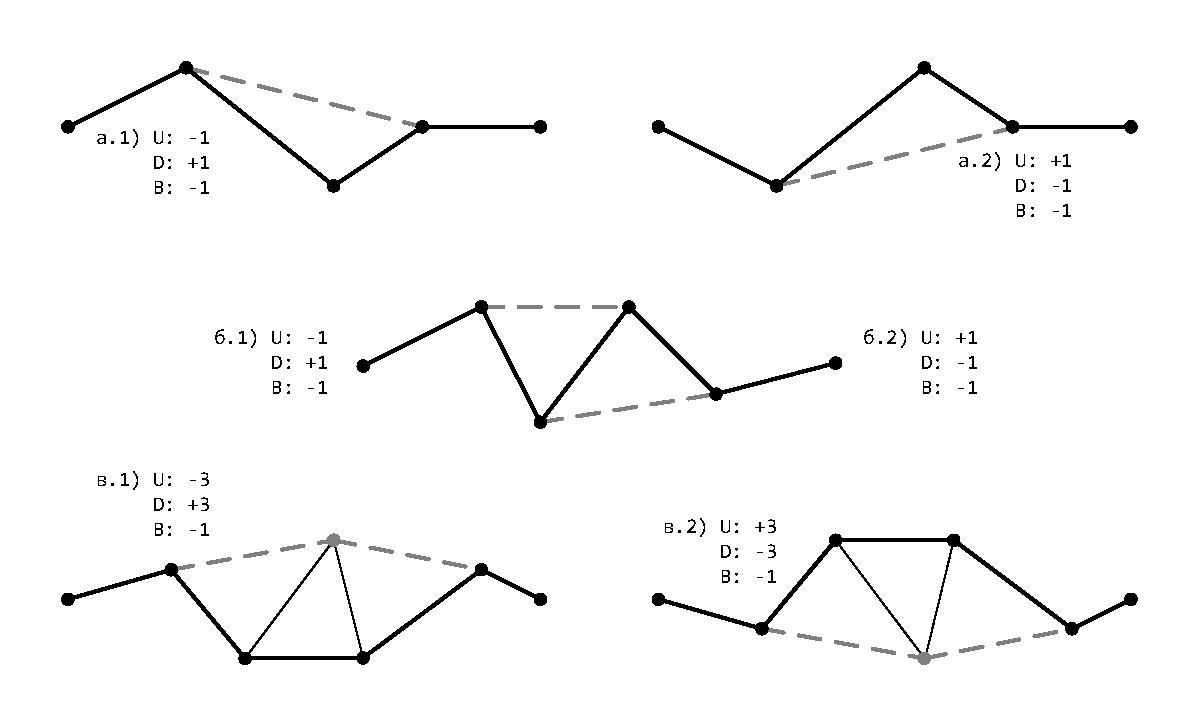
\includegraphics[width=0.8\textwidth]{./pics/text_2_smooth/smooth-border.pdf}
\singlespacing
\captionstyle{center}\caption{Шаблоны элементарных действий сглаживания границ между доменами.}
\label{fig:text_2_smooth_smooth_border}
\end{figure}

На рис.~\ref{fig:text_2_smooth_smooth_border} представлены 5 шаблонов, которые мы будем использовать для уменьшения длины границы между двумя доменами.
Рассмотрим шаблон а.1.
На нем обозначена часть границы между двумя доменами (домен сверху от ломаной обозначен буквой $U$, домен снизу от ломаной обозначен буквой $D$.
Черной сплошной линией прочерчена текущая граница между доменами.
Пунктирной линией показано возможное улучшение, которое в данном случае приведет к следующим последствиям: уменьшение количества ячеек верхнего домена на 1 ($U: -1$), увеличение количества ячеек нижнего домена на 1 ($D: + 1$), уменьшение длины границы между двумя доменами на 1 ($B: -1$).
Таким образом, шаблон а.1 направлен на втягивание одной ячейки из верхнего домена в нижний домен с сокращением длины границы на единицу.
Шаблон а.2 выполняет симметричное действие по втягиванию одной ячейки из нижнего домена в верхний домен, также сокращая при этом длину границы на единицу.
Шаблоны в.1 и в.2 выполняют аналогичные действия, однако вместо одной ячейки происходит втягивание сразу трех соседних ячеек с одновременным уменьшением длины границы между доменами на единицу. Отдельно стоит отметить шаблоны б.1 и б.2.
Они представляют собой один шаблон в рамках которого может быть осуществлено втягивание либо ячейки из нижнего домена в верхний, либо наоборот, но не одновременно (в противном случае длина границы останется неизменной).
Можно рассматривать и более сложные шаблоны, однако существенного прироста производительности они уже не дают, но приводят к усложнению алгоритма.

После того, как внутри цепи найдены все шаблоны, потенциально пригодные для оптимизации границы, выполняется разметка того, как данные шаблоны могут влиять на другие шаблоны.
С учетом того, что любой шаблон может повлиять только на своих непосредственных соседей, такое действие также выполняется с линейной сложностью относительно длины границы.

Последним шагом применения алгоритма является выбор такого множества шаблонов, которые не влияют друг на друга (то есть могут быть применены все одновременно) и не нарушают суммарного баланса ячеек (так как для нас важнейшим показателем эффективности декомпозиции расчетной сетки является равномерность распределения ячеек по доменам).
После выбора наибольшего возможного набора шаблонов они применяются, и на этом обработка цепи считается завершенной.

Рассмотрим более подробно алгоритм выбора максимального подмножества неконфликтующих шаблонов, не нарушающих общий баланс ячеек между парой доменов.
Для этого рассмотрим пример, представленный на рис.~\ref{fig:text_2_smooth_smooth}

\begin{figure}[ht]
\centering
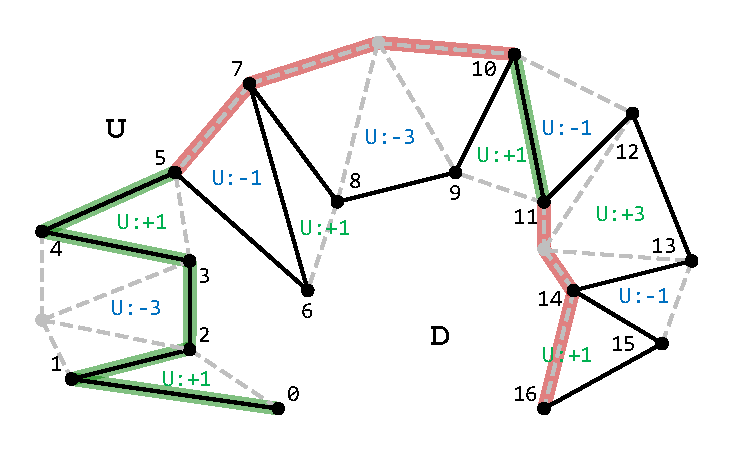
\includegraphics[width=0.8\textwidth]{./pics/text_2_smooth/smooth.pdf}
\singlespacing
\captionstyle{center}\caption{Алгоритм сглаживания границы между доменами.}
\label{fig:text_2_smooth_smooth}
\end{figure}

На рис.~\ref{fig:text_2_smooth_smooth} представлена граница между двумя доменами (они условно обозначены $U$ -- верхний и $D$ -- нижний) в виде простой цепи $0-16$.
Шаблон, который может быть применен для сглаживания границы будем обозначать $t_{a-b}$, где $a$ -- номер стартовой вершины, а $b$ -- номер конечной вершины ($b > a$).
На рис.~\ref{fig:text_2_smooth_smooth} представлены следующие шаблоны
\begin{equation}
T = \{ t_{0-2}, t_{1-4}, t_{3-5}, t_{5-7}, t_{6-8}, t_{7-10}, t_{9-11}, t_{10-12}, t_{11-14}, t_{13-15}, t_{14-16} \}
\end{equation}

Использование каждого из приведенных шаблонов уменьшает длину границы, но нарушает баланс ячеек между доменами.
Будем использовать функцию $U(t)$, которая обозначает изменение баланса ячеек по отношению к домену $U$ из-за применения шаблона $t$.
Так $U(t_{7-10}) = -3$, что означает, что при применении шаблона $t_{7-10}$ домен $U$ потеряет 3 ячейки.

\begin{definition}
Пусть даны два шаблона $t_{a-b}$ и $t_{c-d}$.
Будем говорить, что $t_{a-b} = t_{c-d}$, если $a = c$, $b = d$.
Также будем говорить, что $t_{a-b} < t_{c-d}$, если $a < c$.
\end{definition}

\begin{definition}
Два шаблона $t_{a-b} < t_{c-d}$ назовем конфликтующими (или пересекающимися по ребрам), если $c < b$, и будем обозначать $t_{a-b} \cap t_{c-d} \ne \emptyset$.
\end{definition}

На рис.~\ref{fig:text_2_smooth_smooth} каждая пара соседних шаблонов кроме $\{ t_{3-5}$, $t_{5-7} \}$ является конфликтующей.
Два конфликтующих шаблона применить одновременно нельзя, так как это не приведет к уменьшению длины границы.

\begin{figure}[!ht]
\centering
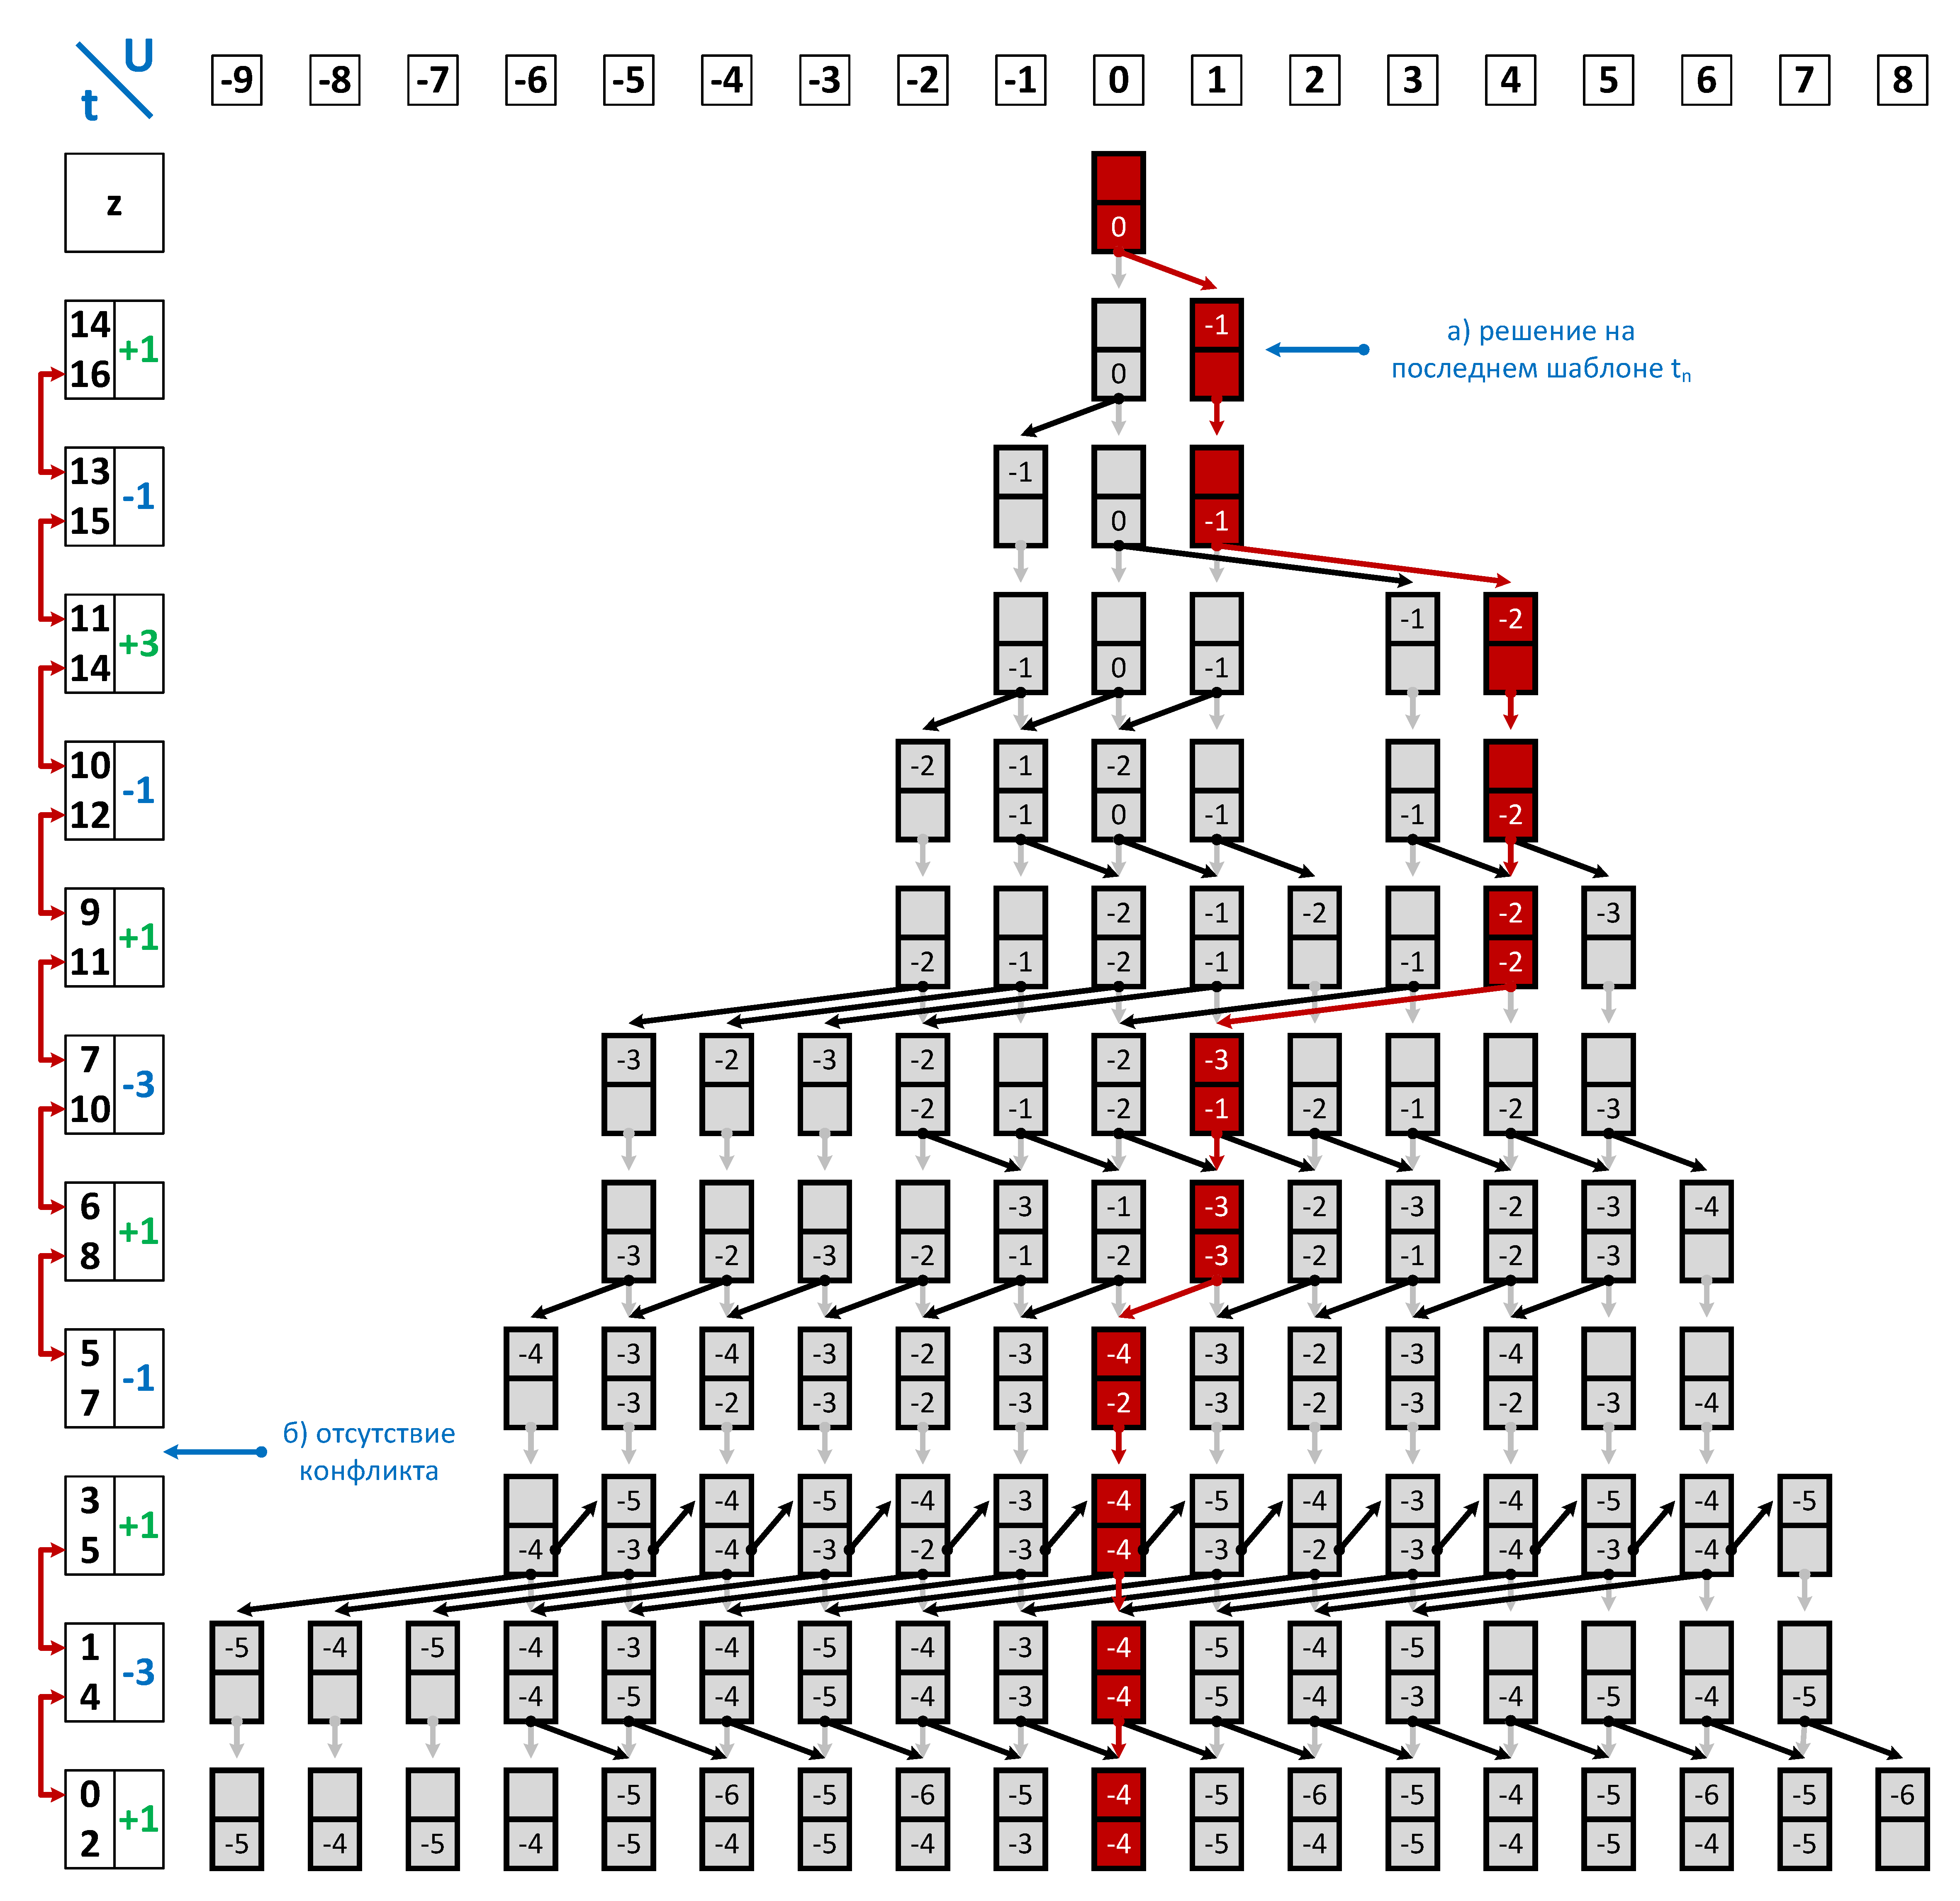
\includegraphics[width=1.0\textwidth]{./pics/text_2_smooth/smooth-scheme-cut.pdf}
\singlespacing
\captionstyle{center}\caption{Схема поиска решения задачи сглаживания границы между доменами.}
\label{fig:text_2_smooth_smooth_scheme}
\end{figure}

Ввиду того, что применение каждого отдельного шаблона уменьшает длину границы на 1, задача поиска оптимального решения может быть сформулирована в виде поиска в множестве шаблонов подмножества максимального размера, не содержащего конфликтующих шаблонов.
Поставленную задачу будем решать методом динамического программирования (схема работы алгоритма для примера с рис.~\ref{fig:text_2_smooth_smooth} представлена на рис.~\ref{fig:text_2_smooth_smooth_scheme}).
Для этого рассмотрим функцию $B(t, u, x)$, отражающую изменение длины границы при решении задачи на множестве шаблонов $\{ t' \in T : t' \ge t \}$ при условии изменения количества ячеек в домене $U$ на $u$ единиц.
Параметр $x$ является булевым и принимает значение $1$, если шаблон $t$ вошел в решение, и $0$ -- в противном случае.
Решением поставленной задачи является значение $\min(B(t_0, 0, 1), B(t_0, 0, 0))$, где $t_0$ -- первый шаблон на рассматриваемой цепи, в нашем случае это $t_{0-2}$.

Решение задачи начинается с последнего шаблона $t_n$ (в нашем случае это $t_{14-16}$) (см. рис.~\ref{fig:text_2_smooth_smooth_scheme}, а).
Для него все множество используемых шаблонов состоит только из него самого, и
\begin{equation}
	\left\{
		\begin{aligned}
			& B(t_n, 0, 0) = 0 \\
			& B(t_n, U(t_n), 1) = -1
		\end{aligned}
	\right.
\end{equation}

для всех остальных значений $u$ значение функции $B(t_n, u, x)$ не определено, будем считать его равным $+\infty$ (это означает, что на последнем шаблоне кроме значений $0$ и $U(t_n)$ недостижимы другие значения изменения количества ячеек в домене $U$).

Пусть задача решена для некоторого шаблона $t_{k + 1}$.
Рассмотрим переход к решению для $t_k$.
Изначально все значения $B(t_k, u, x)$ принимаются равными $+\infty$.

Во-первых, имея любое допустимое решение для шаблона $t_{k + 1}$ мы можем получить решение для шаблона $t_k$, просто проигнорировав этот шаблон, то есть для всех $u$, для которых найдено решение для шаблона $t_{k + 1}$, выполним следующую операцию (на рис.~\ref{fig:text_2_smooth_smooth_scheme} представлена серыми стрелками):
\begin{equation}
	B(t_k, u, 0) = \min \left( B(t_{k + 1}, u, 0), B(t_{k + 1}, u, 1) \right)
\end{equation}

Игнорирование шаблона $t_k$ не меняет баланс ячеек между доменами, из рис.~\ref{fig:text_2_smooth_smooth_scheme} это видно, так как все серые стрелки направлены строго вниз.

Второй момент связан с попыткой использования шаблона $t_k$.
Если $t_k \cap t_{k + 1} = \emptyset$, то есть конфликта нет (см. рис.~\ref{fig:text_2_smooth_smooth_scheme}, б), то шаблон $t_k$ можно использовать вне зависимости от того, был ли использован шаблон $t_{k + 1}$.
То есть для всех $u$, для которых было найдено решение для шаблона $t_{k + 1}$ выполним следующее действие:
\begin{equation}
	B(t_k, u + U(t_k), 1) = B(t_k, u, 0) - 1
\end{equation}

И наконец в случае конфликтующих $t_k$ и $t_{k + 1}$ мы можем использовать шаблон $t_k$ только в том случае, если не был использован шаблон $t_{k + 1}$, то есть для всех $u$ для которых $B(t_{k + 1}, u, 0) \ne +\infty$ нужно выполнить операцию
\begin{equation}
	B(t_k, u + U(t_k), 1) = B(t_{k + 1}, u, 0) - 1
\end{equation}

В результате работы алгоритма получим все наилучшие варианты использования шаблонов для заданного изменения баланса ячеек между доменами $U$ и $D$, в частности для нулевого изменения баланса.
На рис.~\ref{fig:text_2_smooth_smooth_scheme} красным цветом выделен путь для достижения наилучшего сокращения пути при сохранении баланса ячеек между доменами.
В нашем случае одним (но не единственным) из оптимальных решений является использование шаблонов $t_{14-16}$, $t_{11-14}$, $t_{7-10}$, $t_{5-7}$, что сокращает границу между доменами на 4, это решение отражено на рис.~\ref{fig:text_2_smooth_smooth}.

В результате работы алгоритма рассчитываются оптимальные решения для всех значений $u$ из диапазона
\begin{equation}
	[U_{min}, U_{max}] = \left[ \frac{1}{2} \sum_{t \in T}{(U(t) - |U(t)|)}, \frac{1}{2} \sum_{t \in T}{(U(t) + |U(t)|)} \right]
\end{equation}

и его сложность равна $O \left( |T| \cdot (U_{max} - U_{min} + 1) \right)$.

\begin{figure}[ht]
\centering
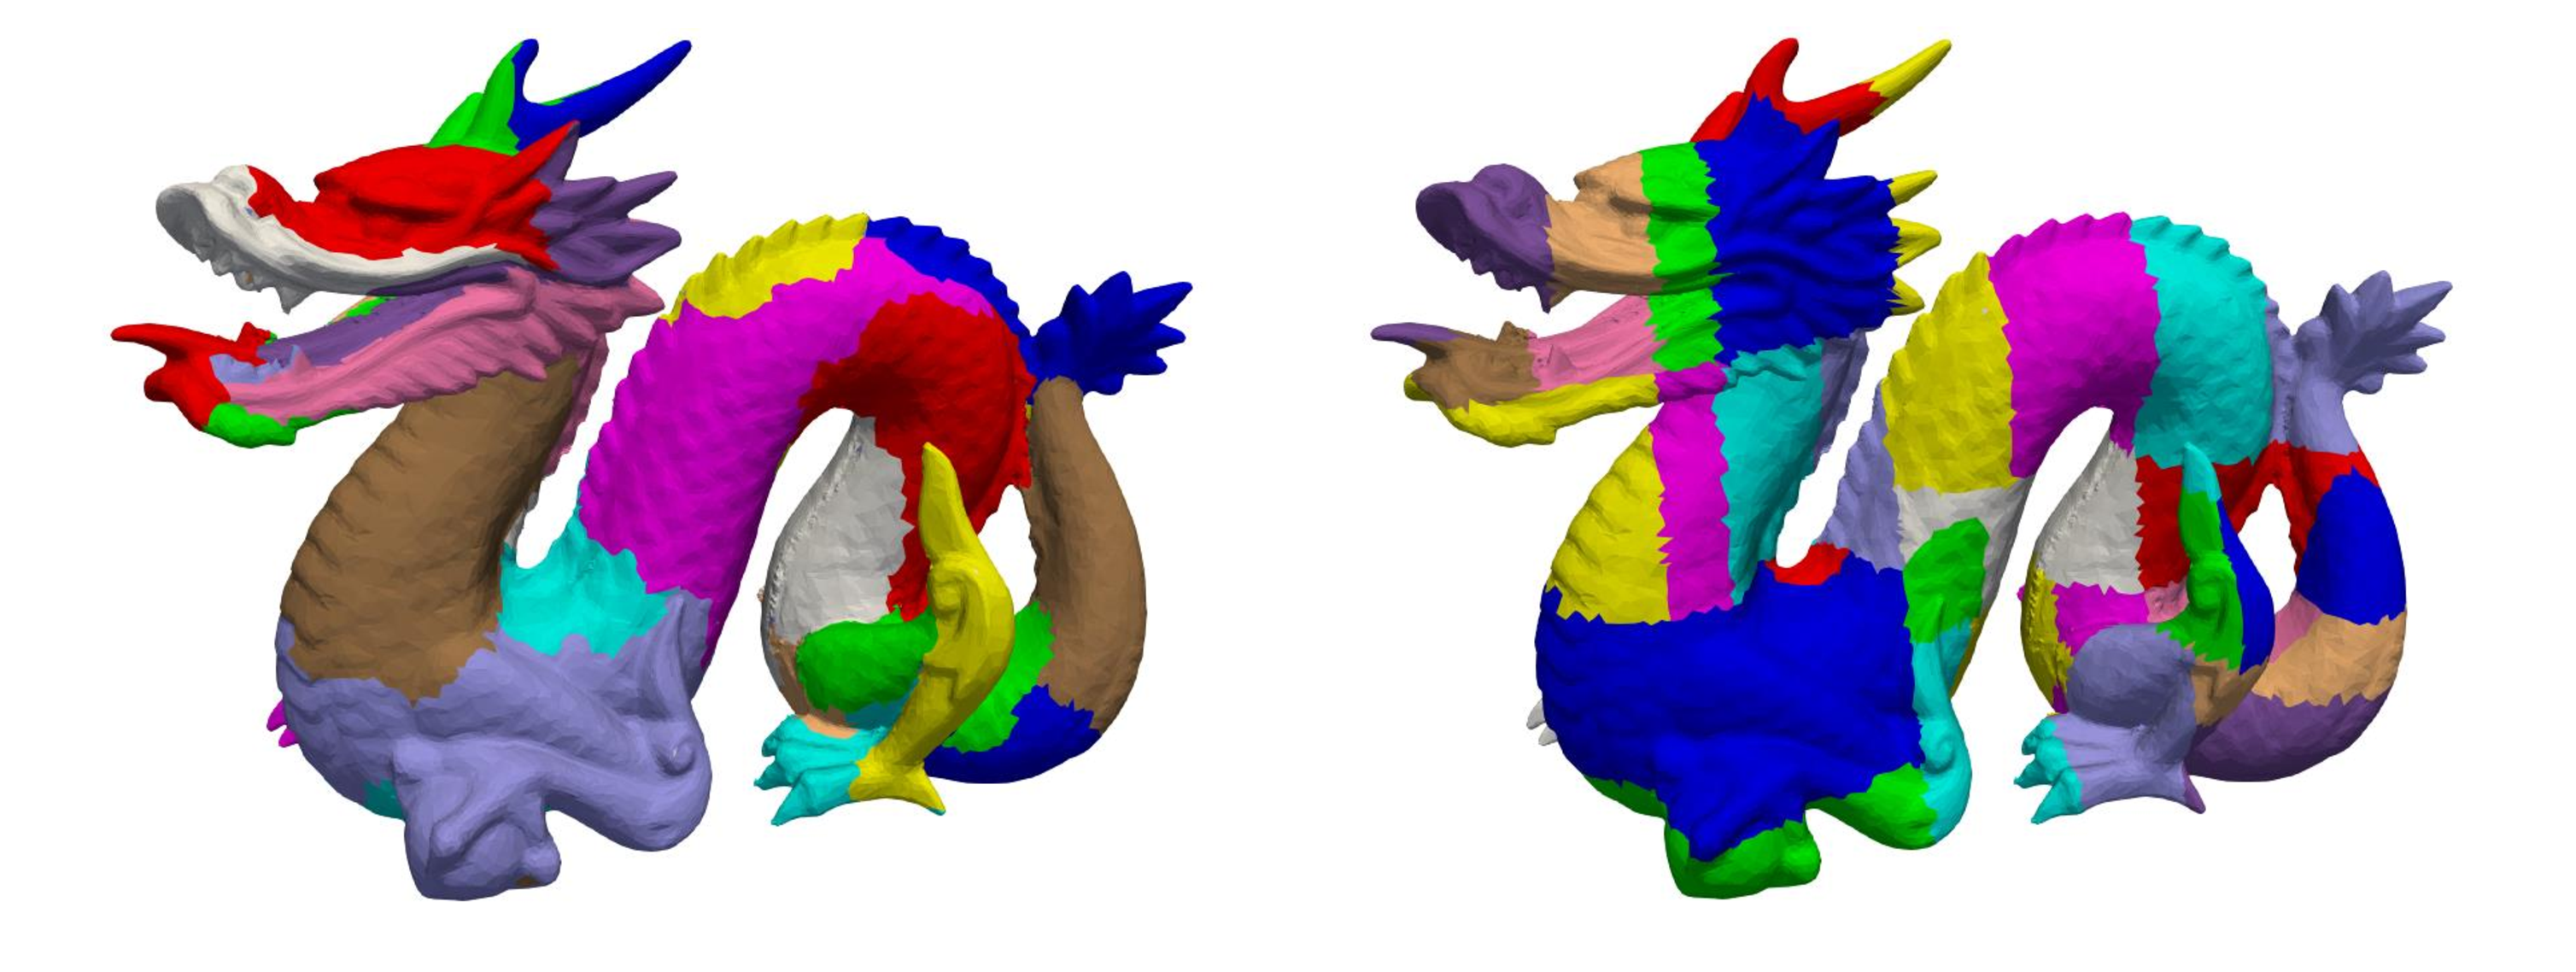
\includegraphics[width=1.0\textwidth]{./pics/text_2_smooth/decomp.pdf}
\singlespacing
\captionstyle{center}\caption{Визуализация декомпозиции тестовой расчетной сетки dragon на 32 домена с помощью алгоритма Фархата (слева) и иерархического алгоритма (справа).}
\label{fig:text_2_smooth_decomp}
\end{figure}

\begin{figure}[!ht]
\centering
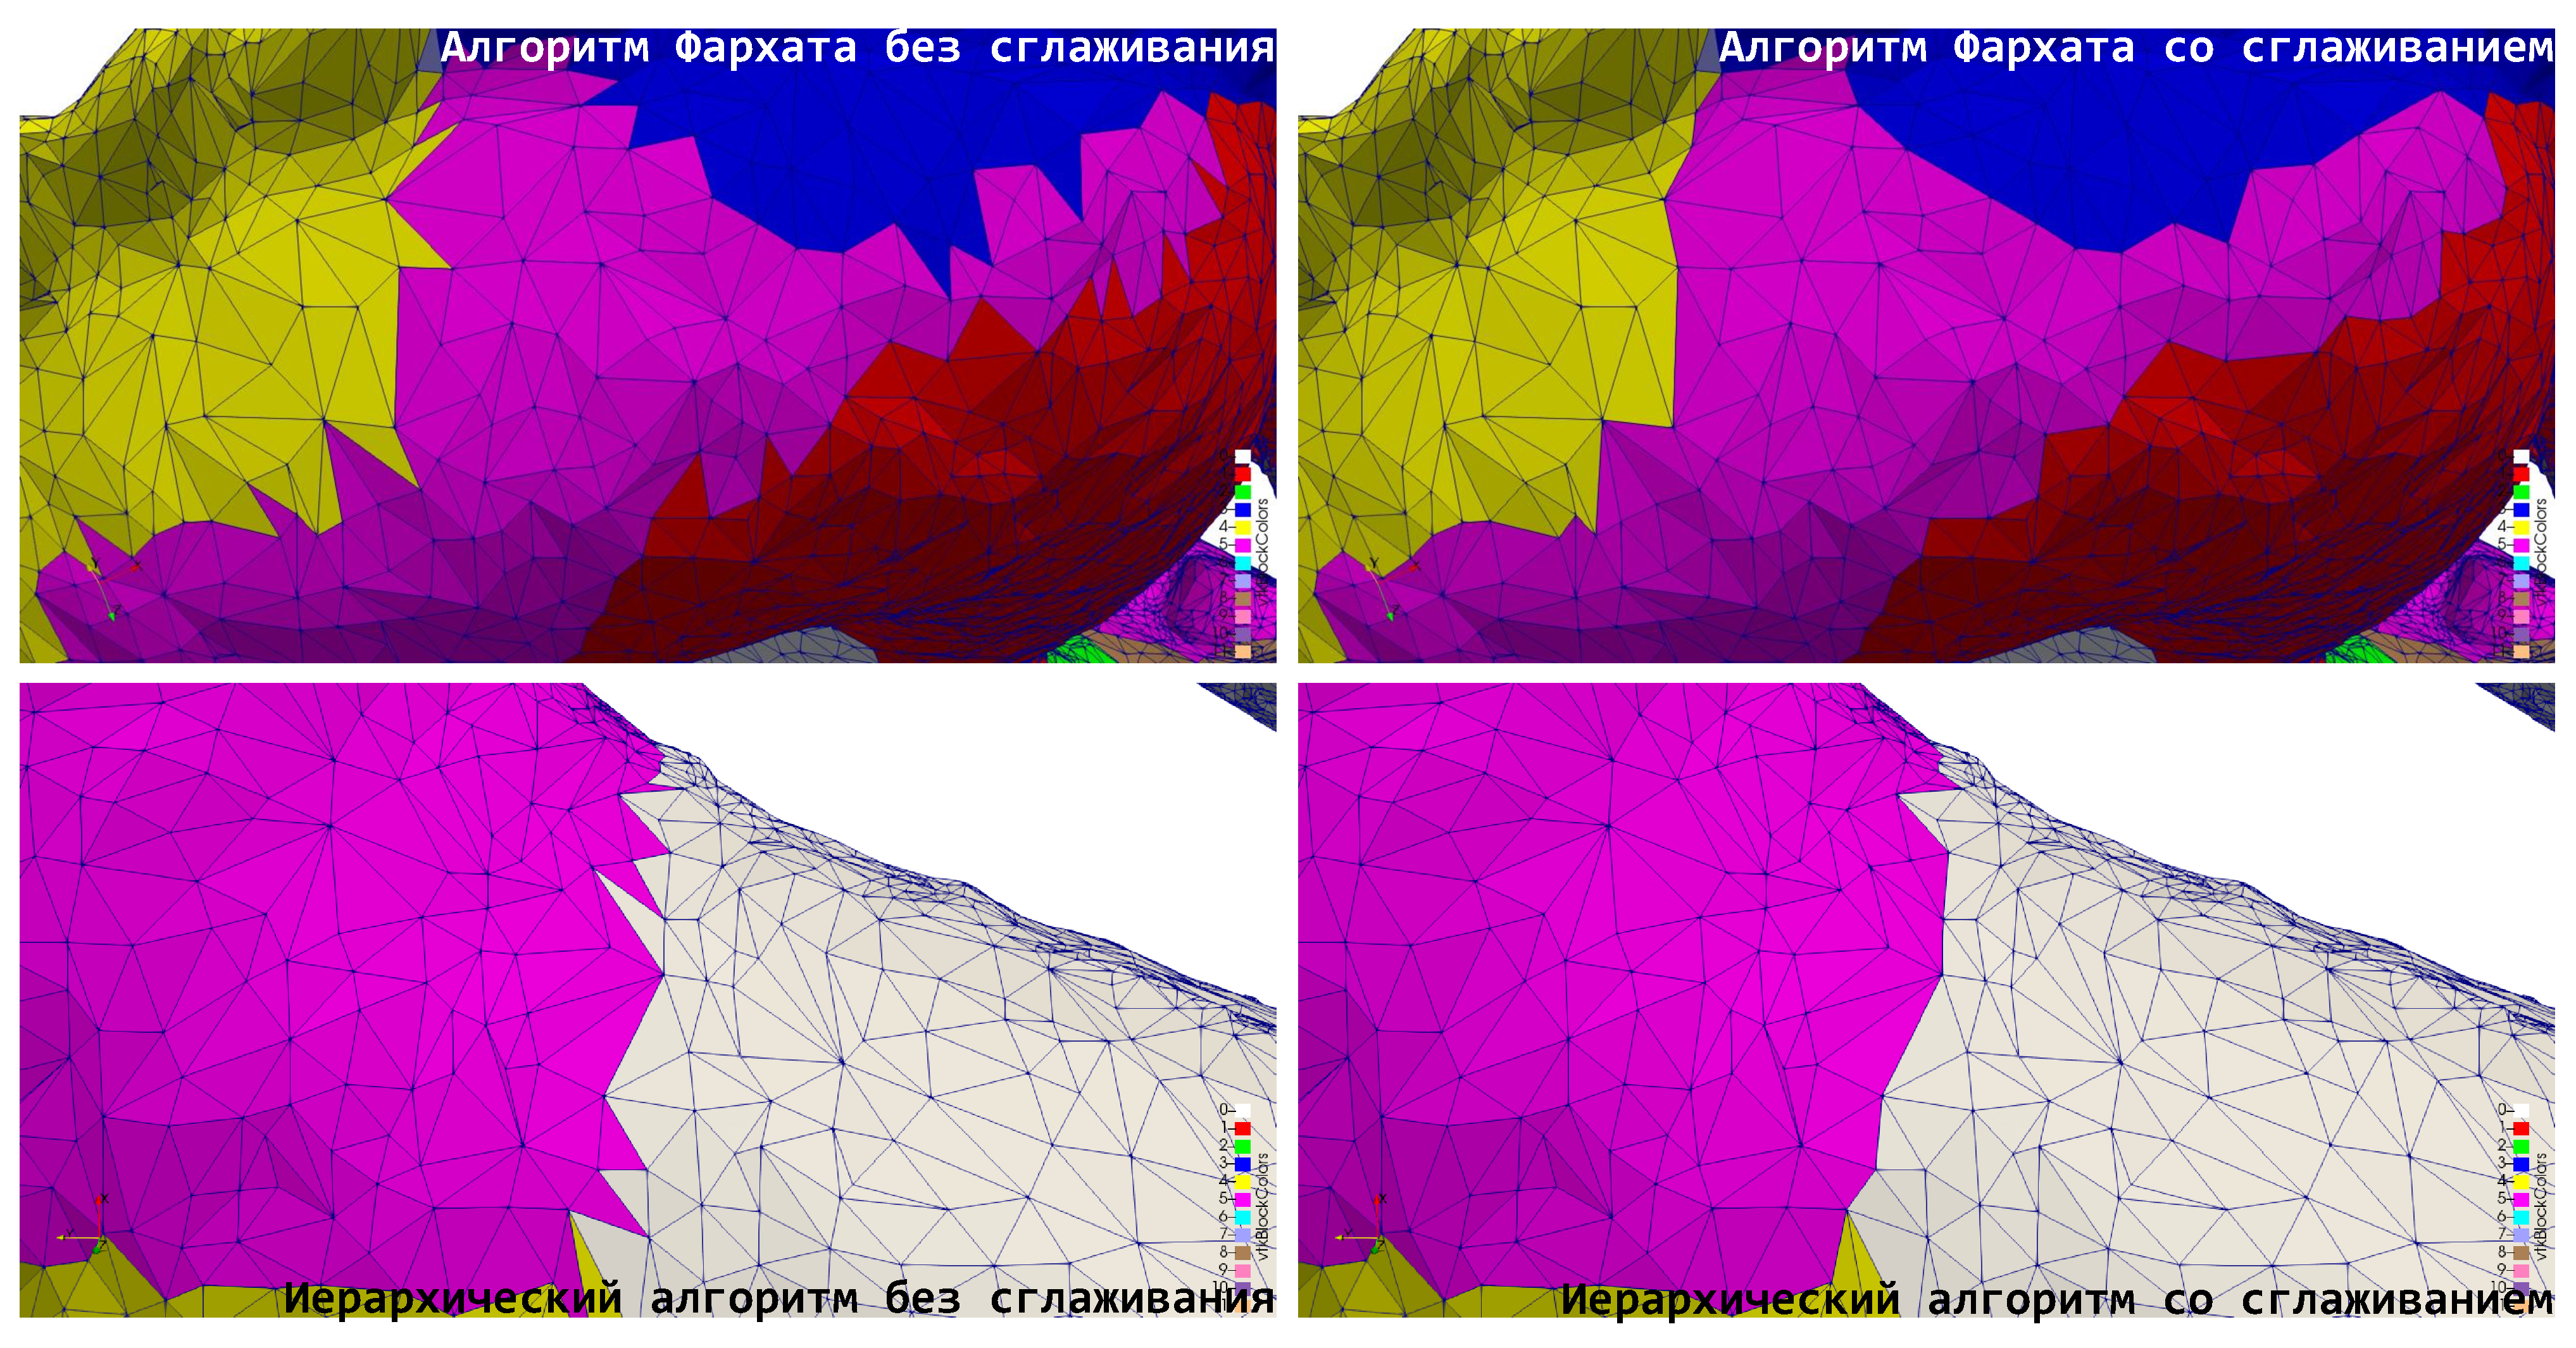
\includegraphics[width=0.8\textwidth]{./pics/text_2_smooth/decomp2.pdf}
\singlespacing
\captionstyle{center}\caption{Визуализация применения сглаживания границ между доменами после работы алгоритма Фархата (сверху) и иерархического алгоритма (снизу).}
\label{fig:text_2_smooth_decomp2}
\end{figure}

На рис.~\ref{fig:text_2_smooth_decomp} представлена визуализация декомпозиции тестовой расчетной сетки dragon с помощью алгоритма Фархата и иерархического алгоритма бинарной декомпозиции.
В обоих случаях декомпозиция выполнятся на 32 домена.
При этом на рис.~\ref{fig:text_2_smooth_decomp2} представлены результаты работы с уже примененным сглаживанием границ между доменами.

На рис.~\ref{fig:text_2_smooth_decomp2} крупным планом продемонстрированы отдельные части тестовой расчетной сетки dragon с отображением ребер ячеек.
На этом рисунке виден эффект от применения алгоритма сглаживания границ меду доменами, прежде всего от заключается в устранении одиноких ячеек, которые вторгаются в соседний домен одной своей вершиной.
После применения алгоритма границы между доменами визуально выглядят более гладко, их длина уменьшается.

\subsubsection{Результаты экспериментов}

Для тестирования эффективности алгоритма сглаживания границ между доменами использовались тестовые неструктурированные поверхностные сетки bunny, dragon, lucy, к которым были применены алгоритмы декомпозиции с показателем $D = 0$\label{term:decomp_neravn6} и сравнены показатели качества декомпозиции до и после сглаживания границ.
Результаты проведения экспериментов представлены на рис.~\ref{fig:text_2_smooth_graphics}.

\begin{figure}[H]
\centering
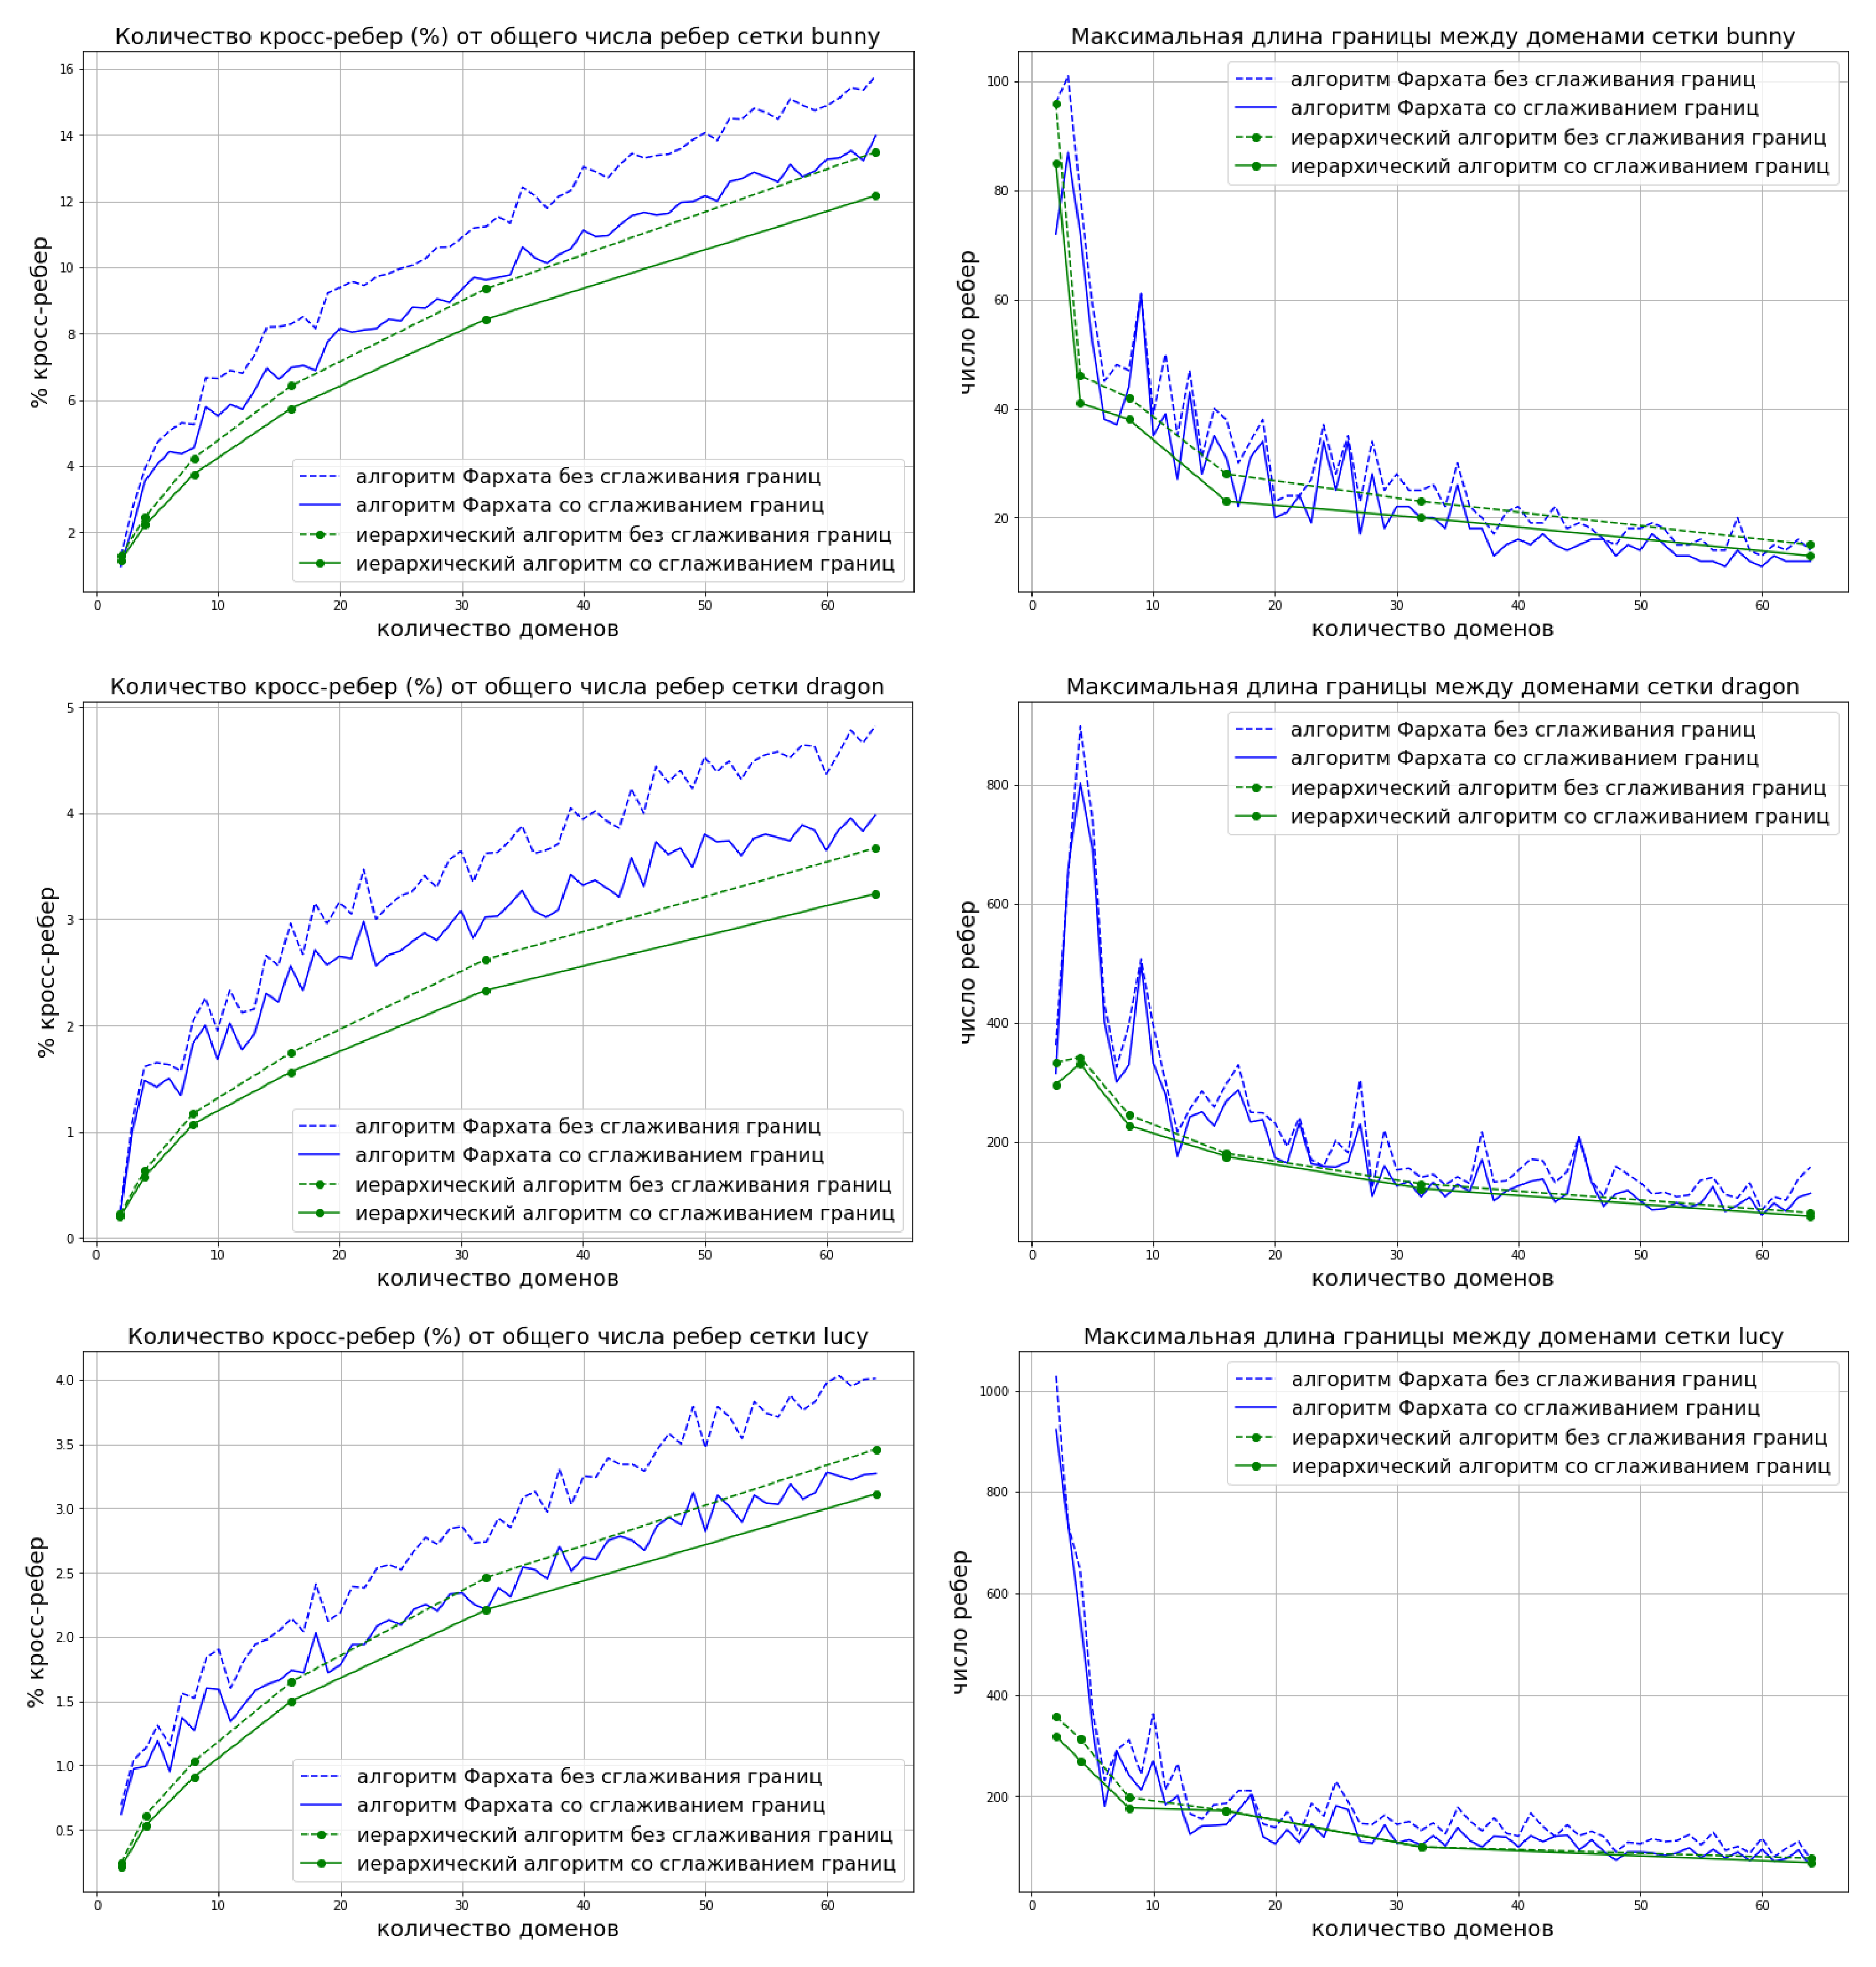
\includegraphics[width=1.0\textwidth]{./pics/text_2_smooth/graphics.pdf}
\singlespacing
\captionstyle{center}\caption{Графики доли кросс-ребер\label{term:edge_cross3} от общего числа ребер сетки (показатель $I^{\%}$\label{term:decomp_sumbord5}) и максимальной длины границы между доменами (показатель $L$\label{term:decomp_maxbord5}) при декомпозиции тестовых сеток bunny, dragon и lucy на количество доменов от 2 до 64.}
\label{fig:text_2_smooth_graphics}
\end{figure}

Неструктурированные поверхностные расчетные сетки bunny (количество ячеек $5 \cdot 10^3$), dragon (количество ячеек $10^5$), lucy (количество ячеек $10^5$) были взяты из открытых источников.
Из приведенных на рис.~\ref{fig:text_2_smooth_graphics} данных видно, что в целом проиллюстрированные показатели эффективности декомпозиции расчетных сеток (процентная доля ребер сетки, являющихся граничными ребрами между доменами, и максимальная длина границы между доменами) лучше для алгоритма иерархического дробления с выбором наилучшего направления в пространстве ($X$, $Y$, $Z$).
Применение же алгоритма сглаживания границ приводит к сокращению как общего количества граничных ребер (кросс-ребер), так и длины максимальной границы примерно на 10\%.
Этот эффект приводит к снижению времени межпроцессных обменов для задач, выполняющих расчеты на поверхностных расчетных сетках\label{term:unstruct_surf_calc_mesh4}.

% Масштабирование вычислений на суперкомпьютере.
\subsubsection{Масштабирование вычислений на поверхностной \\ неструктурированной расчетной сетке}

\subsubsection{Организация межпроцессных обменов}

При проведении расчетов на декомпозированной сетке на каждой итерации счета необходимо выполнять обмен данными на каждой границе между доменами.
В нашем случае при выполнении декомпозиции расчетной сетки граница между двумя доменами представлена произвольным набором междоменных ребер\label{term:edge_cross4}.
При этом граница может быть разрывной, она и вовсе может состоять из отдельных ребер, поэтому последовательность междоменных ребер при описании границы не имеет значения.

На рис.~\ref{fig:text_2_scaling_mpi} представлена схема организации межпроцессных обменов.
На этой иллюстрации два домена (будем условно их называть левым и правым), обрабатывающиеся в MPI-процессах\label{abbr:mpi3} с номерами 0 и 1, разделены границей, состоящей из трех ребер.
При этом в левом домене присутствует три ячейки, которые примыкают к рассматриваемой границе, в правом домене таких ячеек только две (так как ячейка 23R примыкает сразу к двум ребрам границы).
Для организации межпроцессных обменов в каждом домене для каждого ребра рассматриваемой границы создаются фиктивные ячейки, которые участвуют при расчете потоков через ребра границы.
При этом пересчет физических величин в фиктивных ячейках выполнять не требуется, все данные для фиктивных ячеек\label{term:cell_block_ghost2} получаются с помощью MPI-обменов из настоящих ячеек соседнего домена.

\begin{figure}[ht]
\centering
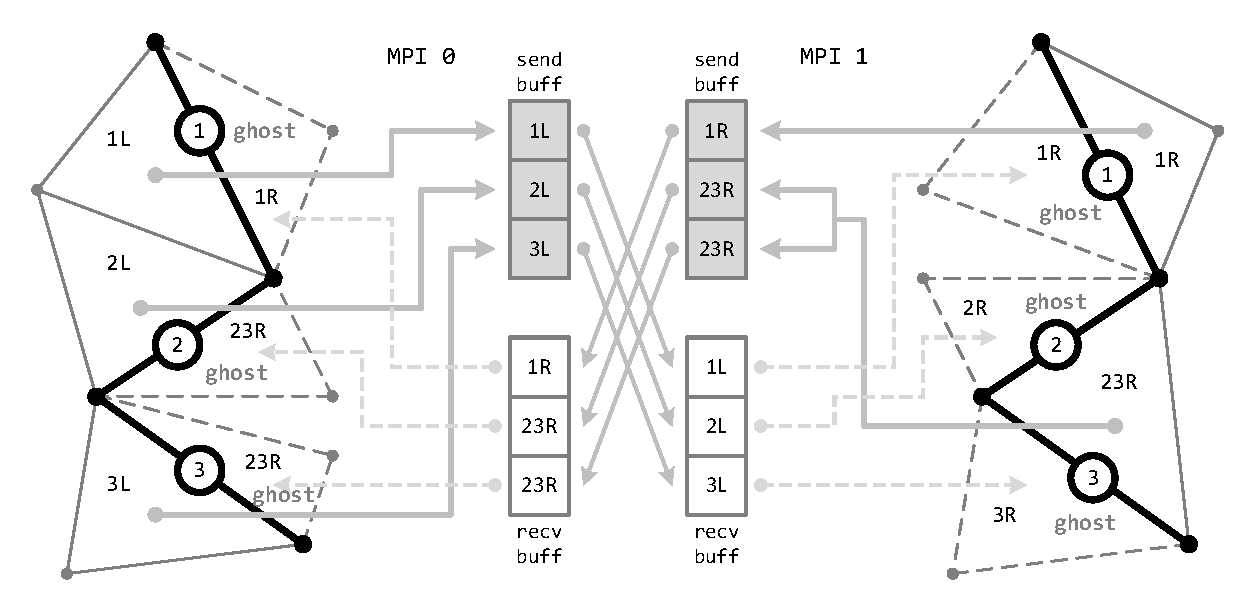
\includegraphics[width=1.0\textwidth]{pics/text_2_scaling/mpi.pdf}
\singlespacing
\captionstyle{center}\caption{Схема выполнения MPI-обменов через границу двух доменов.}\label{fig:text_2_scaling_mpi}
\end{figure}

Для пересылки данных из настоящих граничных ячеек домена в фиктивные ячейки соседнего домена в каждом из двух соседних доменов организуются буферы отправки и приема данных.
Последовательность обмена данными выглядит следующим образом (схема показана на рис.~\ref{fig:text_2_scaling_mpi}).
Сначала данные из настоящих граничных ячеек записываются в соответствующие буферы отправки данных (send buff), далее для всех границ расчетной сетки выполняются асинхронные команды \texttt{MPI\_Irecv} приема сообщений в буферах получения данных (recv buff).
После чего также одновременно для всех границ расчетной сетки выполняются команды асинхронной отправки данных \texttt{MPI\_Isend} из буферов отправки.
Далее выполняется ожидание завершения всех асинхронных обменов данными с помощью функции \texttt{MPI\_Waitall}.
Последним шагом, завершающим обмен данными между соседними доменами, является перенос полученных физических значений из буферов получения данных (recv buff) в соответствующие фиктивные ячейки.

Можно отметить, что при использовании фиктивных ячеек возможно некоторое дублирование данных.
Например, на представленной схеме ячейке 23R из правого домена соответствуют сразу две фиктивные ячейки в левом домене.
Эти ячейки содержат одинаковые данные.
Данное дублирование информации является приемлемым, так как данные фиктивных ячеек используются только на чтение для выполнения вычисления потоков через границу доменов, поэтому в данном случае выполнять какую-либо синхронизацию одинаковых фиктивных ячеек не нужно.

\subsubsection{Эффективность масштабирования вычислений \\ на суперкомпьютере}

Для замеров показателей масштабируемости вычислений на неструктурированной поверхностной расчетной сетке была использована тестовая поверхность обтекаемого трехмерного тела, содержащая порядка $2 \cdot 10^5$ узлов и $4 \cdot 10^5$ ячеек.
В ячейках выполнялись расчеты, связанные с моделированием течения жидкой пленки, решением уравнений теплового баланса на поверхности, а также перестроение и сглаживание поверхности.
Для декомпозиции поверхностной сетки использовался простой иерархических алгоритм деления доменов пополам\label{term:alg_decomp_hierarch3}, описанный в разделе \ref{sec:text_2_decompsurf_hierarchical}, в котором в качестве признаков ячеек брались три координаты центра.
При этом в результате критерием выбора конкретной координаты для деления домена являлась минимизация длины границы между двумя доменами (такой подход позволяет выполнять деление домена по наиболее протяженному направлению).

\begin{table}[!ht]
\centering
\setcaptionmargin{0mm}
\onelinecaptionsfalse
\singlespacing
\captionstyle{center}\caption{Конфигурации узлов суперкомпьютера МВС-10П, на которых производились замеры масштабирования вычислений.}
\bigskip
\begin{tabular}{|c|c|c|c|c|}
\hline
\makecell{Семейство \\
процессоров \\
Intel} & \makecell{Количество\\процессоров\\/ ядер\\/ потоков} & \makecell{Частота\\процессора} & \makecell{Объем\\оперативной\\памяти} & \makecell{AVX-512} \\
\hline\hline
Haswell & 2 / 28 / 56 & 2,6 ГГц & 128 ГБ & нет \\
\hline
Broadwell & 2 / 32 / 64 & 2,6 ГГц & 128 ГБ & нет \\
\hline
Phi KNL & 1 / 72 / 288 & 1,5 ГГц & 96 ГБ & да \\
\hline
Skylake & 2 / 36 / 72 & 3,0 ГГц & 192 ГБ & да \\
\hline
Cascade Lake & 2 / 48 / 96 & 3,0 ГГц & 192 ГБ & да \\
\hline
\end{tabular}
\label{tbl:text_2_scaling_supercomputers}
\end{table}   

Для измерения показателей масштабируемости вычислений использовались гомогенные сегменты вычислительной системы МВС-10П.
Всего расчеты проводились на четырех вычислительных сегментах, характеристики узлов которых приведены в таблице~\ref{tbl:text_2_scaling_supercomputers} (использовались все приведенные узлы кроме Haswell) \cite{Shabanov2021Scaling}.
В этой таблице можно отметить, что все микропроцессоры кроме Intel Xeon Broadwell поддерживают набор инструкций AVX-512, позволяющий использовать специальные 512-битные векторные регистры для эффективной векторизации кода.
Также следует выделить вычислительные узлы на базе микропроцессора Intel Xeon Phi KNL\label{abbr:knl}.
Эти микропроцессоры отличаются большим количеством вычислительных ядер, каждое из которых способно выполнять до 4 потоков, что позволяет эффективно распараллеливать расчетные приложения вплоть до 288 потоков на одном микропроцессоре.

\begin{figure}[ht]
\centering
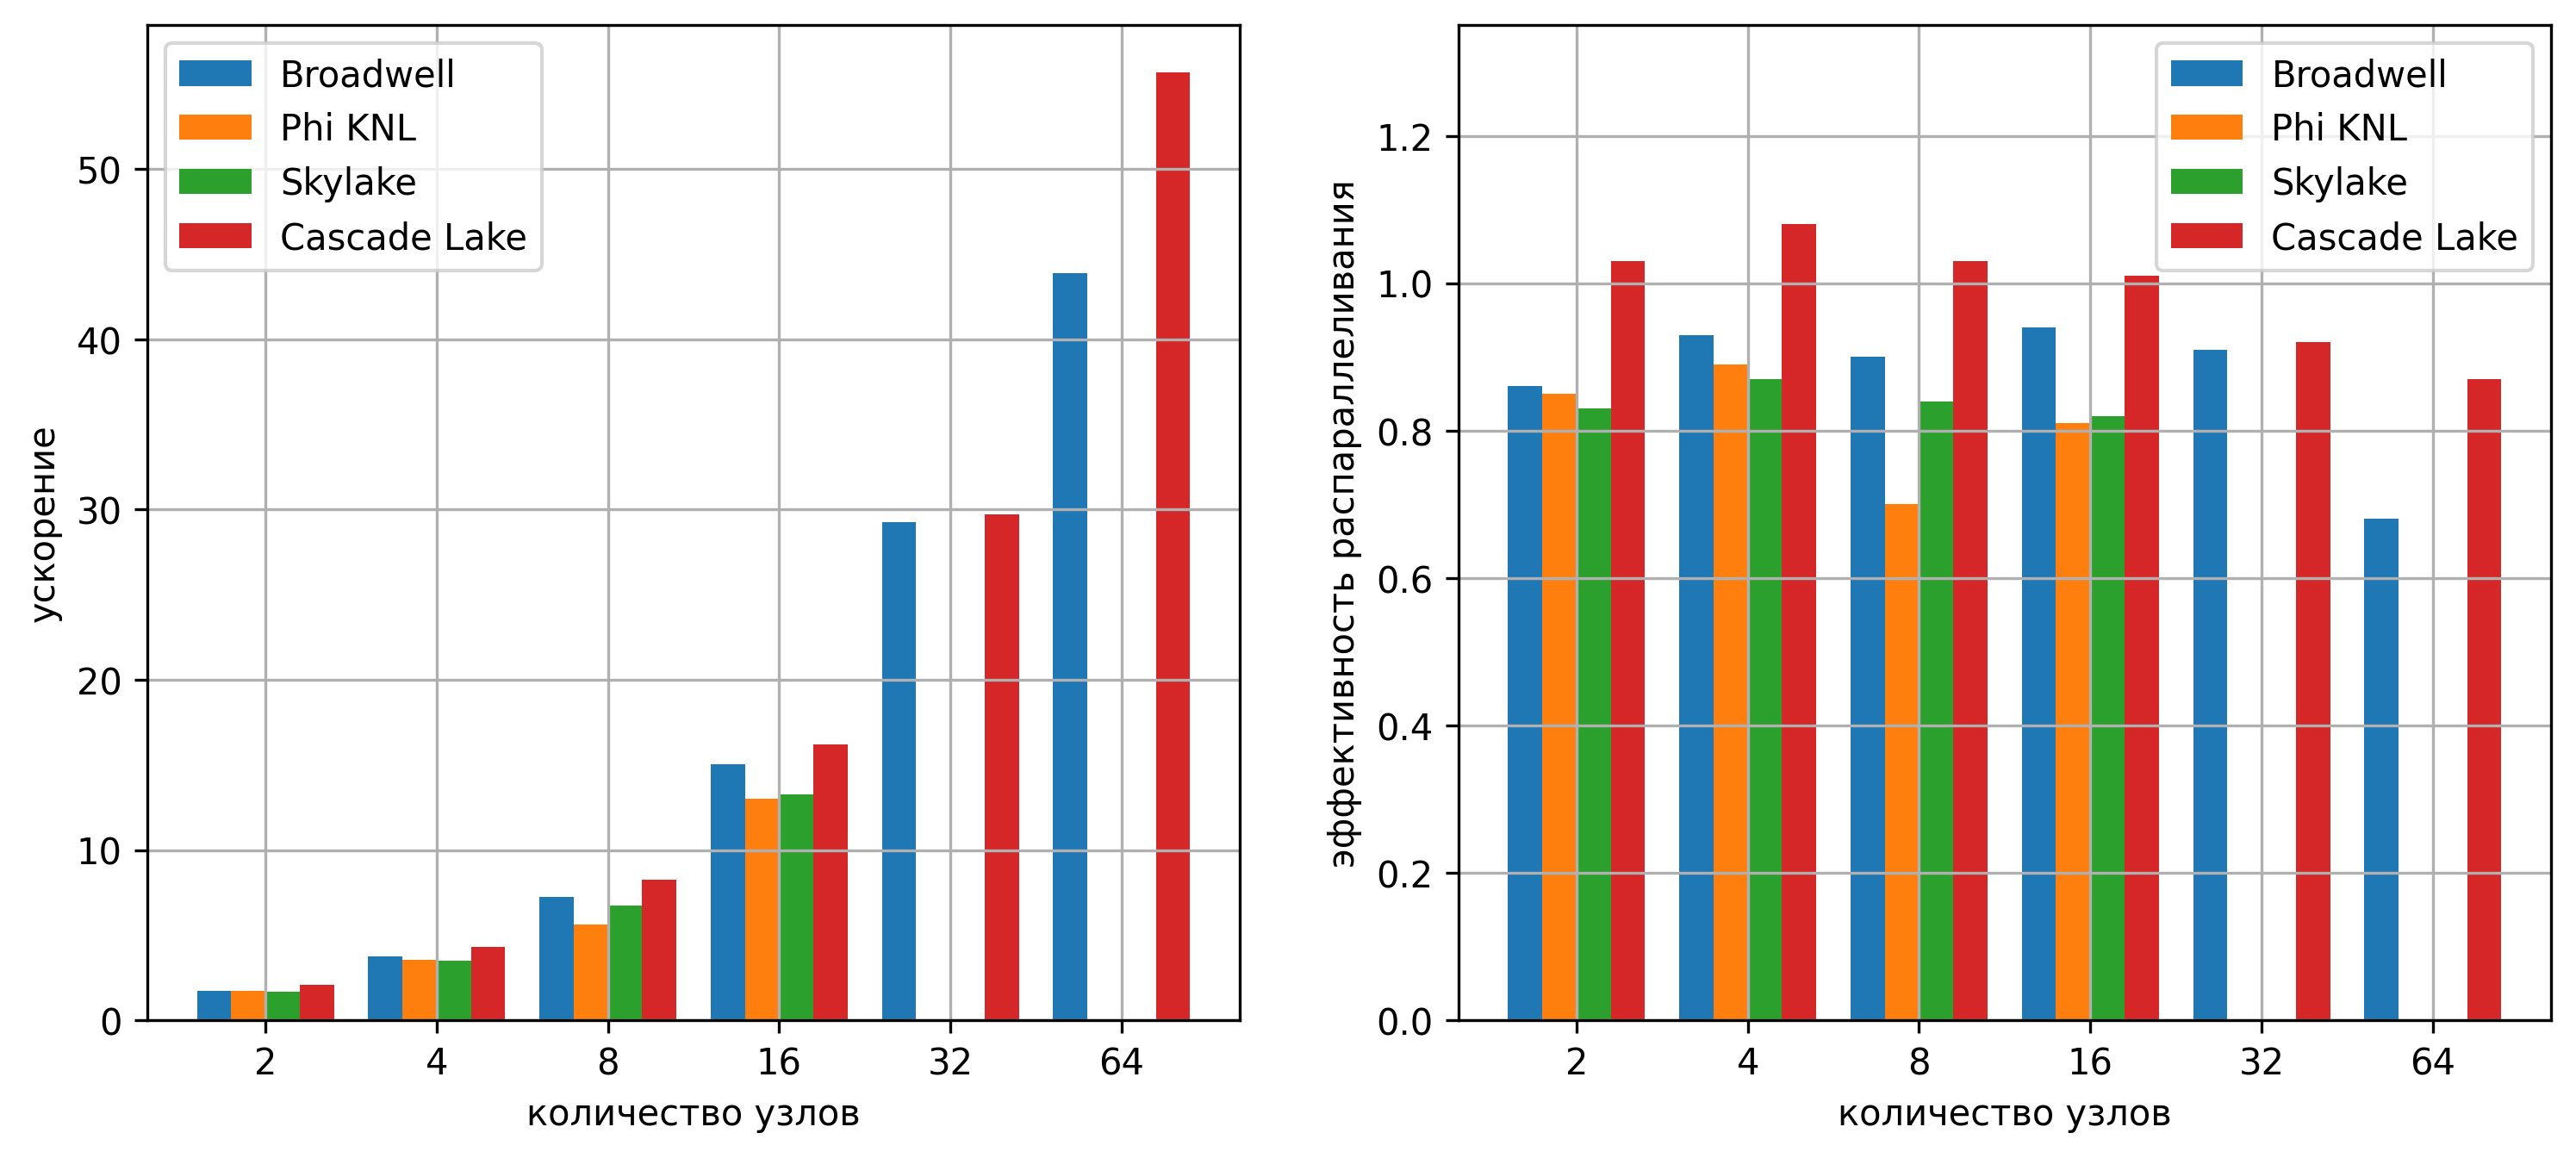
\includegraphics[width=1.0\textwidth]{pics/text_2_scaling/2in1.png}
\singlespacing
\captionstyle{center}\caption{Ускорение (слева) и эффективность распараллеливания (справа) вычислений на сегментах суперкомпьютера МВС-10П при увеличении количества узлов.}
\label{fig:text_2_scaling_speedup_eff}
\end{figure}

Основной целью выполняемых запусков было проведение замеров показателей сильной масштабируемости вычислений при полном распараллеливании внутри вычислительных узлов с использованием OpenMP\label{abbr:openmp}.
То есть для всех запусков использовалась одна и та же поверхность (которая дробилась на нужное количество вычислительных узлов), а также в расчетах были задействованы все потоки, доступные внутри вычислительных узлов.

При проведении расчетов замеры выполнялись независимо для каждой вычислительной системы в отдельности.
На рис.~\ref{fig:text_2_scaling_speedup_eff} приведены диаграммы ускорения вычислений $s_{msg}$\label{term:msg_speedup2} и эффективности распараллеливания $e_{msg}$\label{term:msg_eff2} при увеличении количества вычислительных узлов для разных вычислительных систем.
Можно видеть, что для всех вычислительных систем эффективность масштабирования варьируется в районе значений 0,8-0,9, хотя на некоторых конфигурациях запуска наблюдаются провалы даже в район 0,7.
Запуски с низким значением эффективности распараллеливания как правило связаны с разбросом времени обработки MPI процессами своих доменов.
Заметим, что для сегмента Cascade Lake при количестве узлов 2, 4, 8 и 16 наблюдается проявление сверхлинейной масштабируемости (когда значение $e_{msg}$ поднимается выше единицы), однако это скорее исключение, чем ожидаемый эффект.

Несмотря на то, что использованный в запусках алгоритм декомпозиции расчетной сетки обеспечивал равномерное распределение ячеек по доменам, само время обработки ячейки сильно зависит от ее физических свойств и может отличаться в разы.
По этой причине сбалансировать вычислительную нагрузку на разные вычислительные узлы возможно только в динамическом режиме, что не делалось в рамках данного исследования.
Также отметим высокие показатели эффективности масштабирования вычислений для вычислительных узлов на базе микропроцессоров Xeon Cascade Lake.

%---------------------------------------------------------------------------------------------------
% 4.4 - общая память

\subsection{Методы распараллеливания на общей памяти}

%---------------------------------------------------------------------------------------------------

\subsection{Выводы из главы}

Предложенная архитектура блочно-структу-рированной расчетной сетки с поддержкой дробления блоков и алгоритм распределения блоков по вычислительным процессам позволяет добиться распределения с низким показателем неравномерности при небольшом количестве дроблений блоков.
Предложенный алгоритм сглаживания границ между доменами при декомпозиции поверхностной неструктурированной расчетной сетки позволяет найти точное решение, снизив длины границ примерно на 10\%.
С помощью алгоритмов реберной раскраски дуального графа поверхностной неструктурированной расчетной сетки можно избежать конфликтов по данным при проведении конечно-объемных расчетов на поверхностной сетке.
Результаты экспериментов по масштабированию скалярных и векторных вычислений на общей памяти показали, что векторизация вычислений оправлана при достижении ускорения хотя бы вдвое по сравнению со скарярным кодом.

%---------------------------------------------------------------------------------------------------
